\documentclass[twoside]{book}

% Packages required by doxygen
\usepackage{fixltx2e}
\usepackage{calc}
\usepackage{doxygen}
\usepackage{graphicx}
\usepackage[utf8]{inputenc}
\usepackage{makeidx}
\usepackage{multicol}
\usepackage{multirow}
\PassOptionsToPackage{warn}{textcomp}
\usepackage{textcomp}
\usepackage[nointegrals]{wasysym}
\usepackage[table]{xcolor}

% Font selection
\usepackage[T1]{fontenc}
\usepackage{mathptmx}
\usepackage[scaled=.90]{helvet}
\usepackage{courier}
\usepackage{amssymb}
\usepackage{sectsty}
\renewcommand{\familydefault}{\sfdefault}
\allsectionsfont{%
  \fontseries{bc}\selectfont%
  \color{darkgray}%
}
\renewcommand{\DoxyLabelFont}{%
  \fontseries{bc}\selectfont%
  \color{darkgray}%
}
\newcommand{\+}{\discretionary{\mbox{\scriptsize$\hookleftarrow$}}{}{}}

% Page & text layout
\usepackage{geometry}
\geometry{%
  a4paper,%
  top=2.5cm,%
  bottom=2.5cm,%
  left=2.5cm,%
  right=2.5cm%
}
\tolerance=750
\hfuzz=15pt
\hbadness=750
\setlength{\emergencystretch}{15pt}
\setlength{\parindent}{0cm}
\setlength{\parskip}{0.2cm}
\makeatletter
\renewcommand{\paragraph}{%
  \@startsection{paragraph}{4}{0ex}{-1.0ex}{1.0ex}{%
    \normalfont\normalsize\bfseries\SS@parafont%
  }%
}
\renewcommand{\subparagraph}{%
  \@startsection{subparagraph}{5}{0ex}{-1.0ex}{1.0ex}{%
    \normalfont\normalsize\bfseries\SS@subparafont%
  }%
}
\makeatother

% Headers & footers
\usepackage{fancyhdr}
\pagestyle{fancyplain}
\fancyhead[LE]{\fancyplain{}{\bfseries\thepage}}
\fancyhead[CE]{\fancyplain{}{}}
\fancyhead[RE]{\fancyplain{}{\bfseries\leftmark}}
\fancyhead[LO]{\fancyplain{}{\bfseries\rightmark}}
\fancyhead[CO]{\fancyplain{}{}}
\fancyhead[RO]{\fancyplain{}{\bfseries\thepage}}
\fancyfoot[LE]{\fancyplain{}{}}
\fancyfoot[CE]{\fancyplain{}{}}
\fancyfoot[RE]{\fancyplain{}{\bfseries\scriptsize Generated on Thu Nov 6 2014 17\+:51\+:41 for Media\+Motion by Doxygen }}
\fancyfoot[LO]{\fancyplain{}{\bfseries\scriptsize Generated on Thu Nov 6 2014 17\+:51\+:41 for Media\+Motion by Doxygen }}
\fancyfoot[CO]{\fancyplain{}{}}
\fancyfoot[RO]{\fancyplain{}{}}
\renewcommand{\footrulewidth}{0.4pt}
\renewcommand{\chaptermark}[1]{%
  \markboth{#1}{}%
}
\renewcommand{\sectionmark}[1]{%
  \markright{\thesection\ #1}%
}

% Indices & bibliography
\usepackage{natbib}
\usepackage[titles]{tocloft}
\setcounter{tocdepth}{3}
\setcounter{secnumdepth}{5}
\makeindex

% Hyperlinks (required, but should be loaded last)
\usepackage{ifpdf}
\ifpdf
  \usepackage[pdftex,pagebackref=true]{hyperref}
\else
  \usepackage[ps2pdf,pagebackref=true]{hyperref}
\fi
\hypersetup{%
  colorlinks=true,%
  linkcolor=blue,%
  citecolor=blue,%
  unicode%
}

% Custom commands
\newcommand{\clearemptydoublepage}{%
  \newpage{\pagestyle{empty}\cleardoublepage}%
}


%===== C O N T E N T S =====

\begin{document}

% Titlepage & ToC
\hypersetup{pageanchor=false,
             bookmarks=true,
             bookmarksnumbered=true,
             pdfencoding=unicode
            }
\pagenumbering{roman}
\begin{titlepage}
\vspace*{7cm}
\begin{center}%
{\Large Media\+Motion \\[1ex]\large 0.\+1 }\\
\vspace*{1cm}
{\large Generated by Doxygen 1.8.8}\\
\vspace*{0.5cm}
{\small Thu Nov 6 2014 17:51:41}\\
\end{center}
\end{titlepage}
\clearemptydoublepage
\tableofcontents
\clearemptydoublepage
\pagenumbering{arabic}
\hypersetup{pageanchor=true}

%--- Begin generated contents ---
\chapter{Namespace Index}
\section{Packages}
Here are the packages with brief descriptions (if available)\+:\begin{DoxyCompactList}
\item\contentsline{section}{\hyperlink{namespace_media_motion}{Media\+Motion} }{\pageref{namespace_media_motion}}{}
\item\contentsline{section}{\hyperlink{namespace_media_motion_1_1_core}{Media\+Motion.\+Core} }{\pageref{namespace_media_motion_1_1_core}}{}
\item\contentsline{section}{\hyperlink{namespace_media_motion_1_1_core_1_1_controllers}{Media\+Motion.\+Core.\+Controllers} }{\pageref{namespace_media_motion_1_1_core_1_1_controllers}}{}
\item\contentsline{section}{\hyperlink{namespace_media_motion_1_1_core_1_1_models}{Media\+Motion.\+Core.\+Models} }{\pageref{namespace_media_motion_1_1_core_1_1_models}}{}
\item\contentsline{section}{\hyperlink{namespace_media_motion_1_1_core_1_1_models_1_1_abstract}{Media\+Motion.\+Core.\+Models.\+Abstract} }{\pageref{namespace_media_motion_1_1_core_1_1_models_1_1_abstract}}{}
\item\contentsline{section}{\hyperlink{namespace_media_motion_1_1_core_1_1_models_1_1_enums}{Media\+Motion.\+Core.\+Models.\+Enums} }{\pageref{namespace_media_motion_1_1_core_1_1_models_1_1_enums}}{}
\item\contentsline{section}{\hyperlink{namespace_media_motion_1_1_core_1_1_models_1_1_interfaces}{Media\+Motion.\+Core.\+Models.\+Interfaces} }{\pageref{namespace_media_motion_1_1_core_1_1_models_1_1_interfaces}}{}
\item\contentsline{section}{\hyperlink{namespace_media_motion_1_1_core_1_1_models_1_1_module}{Media\+Motion.\+Core.\+Models.\+Module} }{\pageref{namespace_media_motion_1_1_core_1_1_models_1_1_module}}{}
\item\contentsline{section}{\hyperlink{namespace_media_motion_1_1_core_1_1_models_1_1_module_1_1_interfaces}{Media\+Motion.\+Core.\+Models.\+Module.\+Interfaces} }{\pageref{namespace_media_motion_1_1_core_1_1_models_1_1_module_1_1_interfaces}}{}
\item\contentsline{section}{\hyperlink{namespace_media_motion_1_1_core_1_1_models_1_1_wrapper}{Media\+Motion.\+Core.\+Models.\+Wrapper} }{\pageref{namespace_media_motion_1_1_core_1_1_models_1_1_wrapper}}{}
\item\contentsline{section}{\hyperlink{namespace_media_motion_1_1_core_1_1_models_1_1_wrapper_1_1_interfaces}{Media\+Motion.\+Core.\+Models.\+Wrapper.\+Interfaces} }{\pageref{namespace_media_motion_1_1_core_1_1_models_1_1_wrapper_1_1_interfaces}}{}
\item\contentsline{section}{\hyperlink{namespace_media_motion_1_1_modules}{Media\+Motion.\+Modules} }{\pageref{namespace_media_motion_1_1_modules}}{}
\item\contentsline{section}{\hyperlink{namespace_media_motion_1_1_modules_1_1_components}{Media\+Motion.\+Modules.\+Components} }{\pageref{namespace_media_motion_1_1_modules_1_1_components}}{}
\item\contentsline{section}{\hyperlink{namespace_media_motion_1_1_modules_1_1_components_1_1_playlist}{Media\+Motion.\+Modules.\+Components.\+Playlist} }{\pageref{namespace_media_motion_1_1_modules_1_1_components_1_1_playlist}}{}
\item\contentsline{section}{\hyperlink{namespace_media_motion_1_1_modules_1_1_components_1_1_playlist_1_1_events}{Media\+Motion.\+Modules.\+Components.\+Playlist.\+Events} }{\pageref{namespace_media_motion_1_1_modules_1_1_components_1_1_playlist_1_1_events}}{}
\item\contentsline{section}{\hyperlink{namespace_media_motion_1_1_modules_1_1_components_1_1_rotate}{Media\+Motion.\+Modules.\+Components.\+Rotate} }{\pageref{namespace_media_motion_1_1_modules_1_1_components_1_1_rotate}}{}
\item\contentsline{section}{\hyperlink{namespace_media_motion_1_1_modules_1_1_components_1_1_rotate_1_1_events}{Media\+Motion.\+Modules.\+Components.\+Rotate.\+Events} }{\pageref{namespace_media_motion_1_1_modules_1_1_components_1_1_rotate_1_1_events}}{}
\item\contentsline{section}{\hyperlink{namespace_media_motion_1_1_modules_1_1_components_1_1_volume}{Media\+Motion.\+Modules.\+Components.\+Volume} }{\pageref{namespace_media_motion_1_1_modules_1_1_components_1_1_volume}}{}
\item\contentsline{section}{\hyperlink{namespace_media_motion_1_1_modules_1_1_components_1_1_volume_1_1_events}{Media\+Motion.\+Modules.\+Components.\+Volume.\+Events} }{\pageref{namespace_media_motion_1_1_modules_1_1_components_1_1_volume_1_1_events}}{}
\item\contentsline{section}{\hyperlink{namespace_media_motion_1_1_modules_1_1_components_1_1_zoom}{Media\+Motion.\+Modules.\+Components.\+Zoom} }{\pageref{namespace_media_motion_1_1_modules_1_1_components_1_1_zoom}}{}
\item\contentsline{section}{\hyperlink{namespace_media_motion_1_1_modules_1_1_components_1_1_zoom_1_1_events}{Media\+Motion.\+Modules.\+Components.\+Zoom.\+Events} }{\pageref{namespace_media_motion_1_1_modules_1_1_components_1_1_zoom_1_1_events}}{}
\item\contentsline{section}{\hyperlink{namespace_media_motion_1_1_modules_1_1_image_viewer}{Media\+Motion.\+Modules.\+Image\+Viewer} }{\pageref{namespace_media_motion_1_1_modules_1_1_image_viewer}}{}
\item\contentsline{section}{\hyperlink{namespace_media_motion_1_1_modules_1_1_image_viewer_1_1_interfaces}{Media\+Motion.\+Modules.\+Image\+Viewer.\+Interfaces} }{\pageref{namespace_media_motion_1_1_modules_1_1_image_viewer_1_1_interfaces}}{}
\item\contentsline{section}{\hyperlink{namespace_media_motion_1_1_modules_1_1_media_player}{Media\+Motion.\+Modules.\+Media\+Player} }{\pageref{namespace_media_motion_1_1_modules_1_1_media_player}}{}
\item\contentsline{section}{\hyperlink{namespace_media_motion_1_1_modules_1_1_media_player_1_1_events}{Media\+Motion.\+Modules.\+Media\+Player.\+Events} }{\pageref{namespace_media_motion_1_1_modules_1_1_media_player_1_1_events}}{}
\item\contentsline{section}{\hyperlink{namespace_media_motion_1_1_modules_1_1_media_player_1_1_music_player}{Media\+Motion.\+Modules.\+Media\+Player.\+Music\+Player} }{\pageref{namespace_media_motion_1_1_modules_1_1_media_player_1_1_music_player}}{}
\item\contentsline{section}{\hyperlink{namespace_media_motion_1_1_modules_1_1_media_player_1_1_video_player}{Media\+Motion.\+Modules.\+Media\+Player.\+Video\+Player} }{\pageref{namespace_media_motion_1_1_modules_1_1_media_player_1_1_video_player}}{}
\end{DoxyCompactList}

\chapter{Hierarchical Index}
\section{Class Hierarchy}
This inheritance list is sorted roughly, but not completely, alphabetically\+:\begin{DoxyCompactList}
\item Event\+Args\begin{DoxyCompactList}
\item \contentsline{section}{Media\+Motion.\+Modules.\+Components.\+Playlist.\+Events.\+Playlist\+Change\+Event\+Args}{\pageref{class_media_motion_1_1_modules_1_1_components_1_1_playlist_1_1_events_1_1_playlist_change_event_args}}{}
\item \contentsline{section}{Media\+Motion.\+Modules.\+Components.\+Playlist.\+Events.\+Playlist\+Element\+Change\+Event\+Args}{\pageref{class_media_motion_1_1_modules_1_1_components_1_1_playlist_1_1_events_1_1_playlist_element_change_event_args}}{}
\item \contentsline{section}{Media\+Motion.\+Modules.\+Components.\+Rotate.\+Events.\+Rotate\+Event\+Args}{\pageref{class_media_motion_1_1_modules_1_1_components_1_1_rotate_1_1_events_1_1_rotate_event_args}}{}
\item \contentsline{section}{Media\+Motion.\+Modules.\+Components.\+Volume.\+Events.\+Volume\+Change\+Event\+Args}{\pageref{class_media_motion_1_1_modules_1_1_components_1_1_volume_1_1_events_1_1_volume_change_event_args}}{}
\item \contentsline{section}{Media\+Motion.\+Modules.\+Components.\+Zoom.\+Events.\+Zoom\+Event\+Args}{\pageref{class_media_motion_1_1_modules_1_1_components_1_1_zoom_1_1_events_1_1_zoom_event_args}}{}
\item \contentsline{section}{Media\+Motion.\+Modules.\+Media\+Player.\+Events.\+Media\+Event\+Args}{\pageref{class_media_motion_1_1_modules_1_1_media_player_1_1_events_1_1_media_event_args}}{}
\end{DoxyCompactList}
\item I\+Eelement\+U\+I\begin{DoxyCompactList}
\item \contentsline{section}{I\+File\+U\+I}{\pageref{interface_i_file_u_i}}{}
\begin{DoxyCompactList}
\item \contentsline{section}{File\+U\+I}{\pageref{class_file_u_i}}{}
\end{DoxyCompactList}
\item \contentsline{section}{I\+Folder\+U\+I}{\pageref{interface_i_folder_u_i}}{}
\begin{DoxyCompactList}
\item \contentsline{section}{Folder\+U\+I}{\pageref{class_folder_u_i}}{}
\end{DoxyCompactList}
\end{DoxyCompactList}
\item \contentsline{section}{Media\+Motion.\+Core.\+Models.\+Interfaces.\+I\+Element}{\pageref{interface_media_motion_1_1_core_1_1_models_1_1_interfaces_1_1_i_element}}{}
\begin{DoxyCompactList}
\item \contentsline{section}{Media\+Motion.\+Core.\+Models.\+Interfaces.\+I\+File}{\pageref{interface_media_motion_1_1_core_1_1_models_1_1_interfaces_1_1_i_file}}{}
\begin{DoxyCompactList}
\item \contentsline{section}{Media\+Motion.\+Core.\+Models.\+Abstract.\+A\+File}{\pageref{class_media_motion_1_1_core_1_1_models_1_1_abstract_1_1_a_file}}{}
\begin{DoxyCompactList}
\item \contentsline{section}{Media\+Motion.\+Core.\+Models.\+Image}{\pageref{class_media_motion_1_1_core_1_1_models_1_1_image}}{}
\item \contentsline{section}{Media\+Motion.\+Core.\+Models.\+P\+D\+F}{\pageref{class_media_motion_1_1_core_1_1_models_1_1_p_d_f}}{}
\item \contentsline{section}{Media\+Motion.\+Core.\+Models.\+Regular}{\pageref{class_media_motion_1_1_core_1_1_models_1_1_regular}}{}
\item \contentsline{section}{Media\+Motion.\+Core.\+Models.\+Sound}{\pageref{class_media_motion_1_1_core_1_1_models_1_1_sound}}{}
\item \contentsline{section}{Media\+Motion.\+Core.\+Models.\+Text}{\pageref{class_media_motion_1_1_core_1_1_models_1_1_text}}{}
\item \contentsline{section}{Media\+Motion.\+Core.\+Models.\+Video}{\pageref{class_media_motion_1_1_core_1_1_models_1_1_video}}{}
\end{DoxyCompactList}
\end{DoxyCompactList}
\item \contentsline{section}{Media\+Motion.\+Core.\+Models.\+Interfaces.\+I\+Folder}{\pageref{interface_media_motion_1_1_core_1_1_models_1_1_interfaces_1_1_i_folder}}{}
\end{DoxyCompactList}
\item \contentsline{section}{Media\+Motion.\+Core.\+Models.\+Module.\+Interfaces.\+I\+Module}{\pageref{interface_media_motion_1_1_core_1_1_models_1_1_module_1_1_interfaces_1_1_i_module}}{}
\begin{DoxyCompactList}
\item \contentsline{section}{Media\+Motion.\+Modules.\+Image\+Viewer.\+Interfaces.\+I\+Image\+Viewer}{\pageref{interface_media_motion_1_1_modules_1_1_image_viewer_1_1_interfaces_1_1_i_image_viewer}}{}
\item \contentsline{section}{Media\+Motion.\+Modules.\+Media\+Player.\+I\+Media\+Player}{\pageref{interface_media_motion_1_1_modules_1_1_media_player_1_1_i_media_player}}{}
\begin{DoxyCompactList}
\item \contentsline{section}{Media\+Motion.\+Modules.\+Media\+Player.\+A\+Media\+Player}{\pageref{class_media_motion_1_1_modules_1_1_media_player_1_1_a_media_player}}{}
\begin{DoxyCompactList}
\item \contentsline{section}{Media\+Motion.\+Modules.\+Media\+Player.\+Music\+Player.\+Music\+Player}{\pageref{class_media_motion_1_1_modules_1_1_media_player_1_1_music_player_1_1_music_player}}{}
\item \contentsline{section}{Media\+Motion.\+Modules.\+Media\+Player.\+Video\+Player.\+Video\+Player}{\pageref{class_media_motion_1_1_modules_1_1_media_player_1_1_video_player_1_1_video_player}}{}
\end{DoxyCompactList}
\item \contentsline{section}{Media\+Motion.\+Modules.\+Media\+Player.\+Music\+Player.\+I\+Music\+Player}{\pageref{interface_media_motion_1_1_modules_1_1_media_player_1_1_music_player_1_1_i_music_player}}{}
\begin{DoxyCompactList}
\item \contentsline{section}{Media\+Motion.\+Modules.\+Media\+Player.\+Music\+Player.\+Music\+Player}{\pageref{class_media_motion_1_1_modules_1_1_media_player_1_1_music_player_1_1_music_player}}{}
\end{DoxyCompactList}
\item \contentsline{section}{Media\+Motion.\+Modules.\+Media\+Player.\+Video\+Player.\+I\+Video\+Player}{\pageref{interface_media_motion_1_1_modules_1_1_media_player_1_1_video_player_1_1_i_video_player}}{}
\begin{DoxyCompactList}
\item \contentsline{section}{Media\+Motion.\+Modules.\+Media\+Player.\+Video\+Player.\+Video\+Player}{\pageref{class_media_motion_1_1_modules_1_1_media_player_1_1_video_player_1_1_video_player}}{}
\end{DoxyCompactList}
\end{DoxyCompactList}
\end{DoxyCompactList}
\item \contentsline{section}{Media\+Motion.\+Modules.\+Components.\+Playlist.\+I\+Playlist}{\pageref{interface_media_motion_1_1_modules_1_1_components_1_1_playlist_1_1_i_playlist}}{}
\begin{DoxyCompactList}
\item \contentsline{section}{Media\+Motion.\+Modules.\+Components.\+Playlist.\+Playlist}{\pageref{class_media_motion_1_1_modules_1_1_components_1_1_playlist_1_1_playlist}}{}
\item \contentsline{section}{Media\+Motion.\+Modules.\+Image\+Viewer.\+Interfaces.\+I\+Image\+Viewer}{\pageref{interface_media_motion_1_1_modules_1_1_image_viewer_1_1_interfaces_1_1_i_image_viewer}}{}
\item \contentsline{section}{Media\+Motion.\+Modules.\+Media\+Player.\+I\+Media\+Player}{\pageref{interface_media_motion_1_1_modules_1_1_media_player_1_1_i_media_player}}{}
\end{DoxyCompactList}
\item \contentsline{section}{Media\+Motion.\+Modules.\+Components.\+Rotate.\+I\+Rotate}{\pageref{interface_media_motion_1_1_modules_1_1_components_1_1_rotate_1_1_i_rotate}}{}
\begin{DoxyCompactList}
\item \contentsline{section}{Media\+Motion.\+Modules.\+Components.\+Rotate.\+Rotate}{\pageref{class_media_motion_1_1_modules_1_1_components_1_1_rotate_1_1_rotate}}{}
\item \contentsline{section}{Media\+Motion.\+Modules.\+Image\+Viewer.\+Interfaces.\+I\+Image\+Viewer}{\pageref{interface_media_motion_1_1_modules_1_1_image_viewer_1_1_interfaces_1_1_i_image_viewer}}{}
\end{DoxyCompactList}
\item \contentsline{section}{Media\+Motion.\+Modules.\+Components.\+Volume.\+I\+Volume}{\pageref{interface_media_motion_1_1_modules_1_1_components_1_1_volume_1_1_i_volume}}{}
\begin{DoxyCompactList}
\item \contentsline{section}{Media\+Motion.\+Modules.\+Components.\+Volume.\+Volume}{\pageref{class_media_motion_1_1_modules_1_1_components_1_1_volume_1_1_volume}}{}
\item \contentsline{section}{Media\+Motion.\+Modules.\+Media\+Player.\+I\+Media\+Player}{\pageref{interface_media_motion_1_1_modules_1_1_media_player_1_1_i_media_player}}{}
\end{DoxyCompactList}
\item \contentsline{section}{Media\+Motion.\+Core.\+Models.\+Wrapper.\+Interfaces.\+I\+Wrapper}{\pageref{interface_media_motion_1_1_core_1_1_models_1_1_wrapper_1_1_interfaces_1_1_i_wrapper}}{}
\item \contentsline{section}{Media\+Motion.\+Modules.\+Components.\+Zoom.\+I\+Zoom}{\pageref{interface_media_motion_1_1_modules_1_1_components_1_1_zoom_1_1_i_zoom}}{}
\begin{DoxyCompactList}
\item \contentsline{section}{Media\+Motion.\+Modules.\+Image\+Viewer.\+Interfaces.\+I\+Image\+Viewer}{\pageref{interface_media_motion_1_1_modules_1_1_image_viewer_1_1_interfaces_1_1_i_image_viewer}}{}
\end{DoxyCompactList}
\item Mono\+Behaviour\begin{DoxyCompactList}
\item \contentsline{section}{I\+Element\+U\+I}{\pageref{interface_i_element_u_i}}{}
\begin{DoxyCompactList}
\item \contentsline{section}{Element\+U\+I}{\pageref{class_element_u_i}}{}
\end{DoxyCompactList}
\item \contentsline{section}{I\+Folder\+Content\+U\+I}{\pageref{interface_i_folder_content_u_i}}{}
\begin{DoxyCompactList}
\item \contentsline{section}{Folder\+Content\+U\+I}{\pageref{class_folder_content_u_i}}{}
\end{DoxyCompactList}
\item \contentsline{section}{I\+Image\+Viewer\+U\+I}{\pageref{interface_i_image_viewer_u_i}}{}
\begin{DoxyCompactList}
\item \contentsline{section}{Image\+Viewer\+U\+I}{\pageref{class_image_viewer_u_i}}{}
\end{DoxyCompactList}
\item \contentsline{section}{I\+Media\+Player\+U\+I}{\pageref{interface_i_media_player_u_i}}{}
\begin{DoxyCompactList}
\item \contentsline{section}{Media\+Player\+U\+I}{\pageref{class_media_player_u_i}}{}
\end{DoxyCompactList}
\item \contentsline{section}{I\+Text\+Reader\+U\+I}{\pageref{interface_i_text_reader_u_i}}{}
\begin{DoxyCompactList}
\item \contentsline{section}{Text\+Reader\+U\+I}{\pageref{class_text_reader_u_i}}{}
\end{DoxyCompactList}
\item \contentsline{section}{I\+Wheel\+Tool\+U\+I}{\pageref{interface_i_wheel_tool_u_i}}{}
\begin{DoxyCompactList}
\item \contentsline{section}{Wheel\+Tool\+U\+I}{\pageref{class_wheel_tool_u_i}}{}
\end{DoxyCompactList}
\item \contentsline{section}{Media\+Motion.\+Core.\+Controllers.\+Folder\+Content\+Controller}{\pageref{class_media_motion_1_1_core_1_1_controllers_1_1_folder_content_controller}}{}
\item \contentsline{section}{Media\+Motion.\+Core.\+Controllers.\+Media\+Motion\+Controller}{\pageref{class_media_motion_1_1_core_1_1_controllers_1_1_media_motion_controller}}{}
\item \contentsline{section}{Media\+Motion.\+Core.\+Controllers.\+Wheel\+Tool\+Controller}{\pageref{class_media_motion_1_1_core_1_1_controllers_1_1_wheel_tool_controller}}{}
\end{DoxyCompactList}
\item \contentsline{section}{Media\+Motion.\+Modules.\+Components.\+Zoom.\+Zoom}{\pageref{class_media_motion_1_1_modules_1_1_components_1_1_zoom_1_1_zoom}}{}
\end{DoxyCompactList}

\chapter{Class Index}
\section{Class List}
Here are the classes, structs, unions and interfaces with brief descriptions\+:\begin{DoxyCompactList}
\item\contentsline{section}{\hyperlink{class_media_motion_1_1_core_1_1_models_1_1_abstract_1_1_a_file}{Media\+Motion.\+Core.\+Models.\+Abstract.\+A\+File} }{\pageref{class_media_motion_1_1_core_1_1_models_1_1_abstract_1_1_a_file}}{}
\item\contentsline{section}{\hyperlink{class_media_motion_1_1_modules_1_1_media_player_1_1_a_media_player}{Media\+Motion.\+Modules.\+Media\+Player.\+A\+Media\+Player} }{\pageref{class_media_motion_1_1_modules_1_1_media_player_1_1_a_media_player}}{}
\item\contentsline{section}{\hyperlink{class_element_u_i}{Element\+U\+I} }{\pageref{class_element_u_i}}{}
\item\contentsline{section}{\hyperlink{class_file_u_i}{File\+U\+I} }{\pageref{class_file_u_i}}{}
\item\contentsline{section}{\hyperlink{class_media_motion_1_1_core_1_1_controllers_1_1_folder_content_controller}{Media\+Motion.\+Core.\+Controllers.\+Folder\+Content\+Controller} }{\pageref{class_media_motion_1_1_core_1_1_controllers_1_1_folder_content_controller}}{}
\item\contentsline{section}{\hyperlink{class_folder_content_u_i}{Folder\+Content\+U\+I} }{\pageref{class_folder_content_u_i}}{}
\item\contentsline{section}{\hyperlink{class_folder_u_i}{Folder\+U\+I} }{\pageref{class_folder_u_i}}{}
\item\contentsline{section}{\hyperlink{interface_media_motion_1_1_core_1_1_models_1_1_interfaces_1_1_i_element}{Media\+Motion.\+Core.\+Models.\+Interfaces.\+I\+Element} }{\pageref{interface_media_motion_1_1_core_1_1_models_1_1_interfaces_1_1_i_element}}{}
\item\contentsline{section}{\hyperlink{interface_i_element_u_i}{I\+Element\+U\+I} }{\pageref{interface_i_element_u_i}}{}
\item\contentsline{section}{\hyperlink{interface_media_motion_1_1_core_1_1_models_1_1_interfaces_1_1_i_file}{Media\+Motion.\+Core.\+Models.\+Interfaces.\+I\+File} }{\pageref{interface_media_motion_1_1_core_1_1_models_1_1_interfaces_1_1_i_file}}{}
\item\contentsline{section}{\hyperlink{interface_i_file_u_i}{I\+File\+U\+I} }{\pageref{interface_i_file_u_i}}{}
\item\contentsline{section}{\hyperlink{interface_media_motion_1_1_core_1_1_models_1_1_interfaces_1_1_i_folder}{Media\+Motion.\+Core.\+Models.\+Interfaces.\+I\+Folder} }{\pageref{interface_media_motion_1_1_core_1_1_models_1_1_interfaces_1_1_i_folder}}{}
\item\contentsline{section}{\hyperlink{interface_i_folder_content_u_i}{I\+Folder\+Content\+U\+I} }{\pageref{interface_i_folder_content_u_i}}{}
\item\contentsline{section}{\hyperlink{interface_i_folder_u_i}{I\+Folder\+U\+I} }{\pageref{interface_i_folder_u_i}}{}
\item\contentsline{section}{\hyperlink{interface_media_motion_1_1_modules_1_1_image_viewer_1_1_interfaces_1_1_i_image_viewer}{Media\+Motion.\+Modules.\+Image\+Viewer.\+Interfaces.\+I\+Image\+Viewer} }{\pageref{interface_media_motion_1_1_modules_1_1_image_viewer_1_1_interfaces_1_1_i_image_viewer}}{}
\item\contentsline{section}{\hyperlink{interface_i_image_viewer_u_i}{I\+Image\+Viewer\+U\+I} }{\pageref{interface_i_image_viewer_u_i}}{}
\item\contentsline{section}{\hyperlink{class_media_motion_1_1_core_1_1_models_1_1_image}{Media\+Motion.\+Core.\+Models.\+Image} }{\pageref{class_media_motion_1_1_core_1_1_models_1_1_image}}{}
\item\contentsline{section}{\hyperlink{class_image_viewer_u_i}{Image\+Viewer\+U\+I} }{\pageref{class_image_viewer_u_i}}{}
\item\contentsline{section}{\hyperlink{interface_media_motion_1_1_modules_1_1_media_player_1_1_i_media_player}{Media\+Motion.\+Modules.\+Media\+Player.\+I\+Media\+Player} }{\pageref{interface_media_motion_1_1_modules_1_1_media_player_1_1_i_media_player}}{}
\item\contentsline{section}{\hyperlink{interface_i_media_player_u_i}{I\+Media\+Player\+U\+I} }{\pageref{interface_i_media_player_u_i}}{}
\item\contentsline{section}{\hyperlink{interface_media_motion_1_1_core_1_1_models_1_1_module_1_1_interfaces_1_1_i_module}{Media\+Motion.\+Core.\+Models.\+Module.\+Interfaces.\+I\+Module} }{\pageref{interface_media_motion_1_1_core_1_1_models_1_1_module_1_1_interfaces_1_1_i_module}}{}
\item\contentsline{section}{\hyperlink{interface_media_motion_1_1_modules_1_1_media_player_1_1_music_player_1_1_i_music_player}{Media\+Motion.\+Modules.\+Media\+Player.\+Music\+Player.\+I\+Music\+Player} }{\pageref{interface_media_motion_1_1_modules_1_1_media_player_1_1_music_player_1_1_i_music_player}}{}
\item\contentsline{section}{\hyperlink{interface_media_motion_1_1_modules_1_1_components_1_1_playlist_1_1_i_playlist}{Media\+Motion.\+Modules.\+Components.\+Playlist.\+I\+Playlist} }{\pageref{interface_media_motion_1_1_modules_1_1_components_1_1_playlist_1_1_i_playlist}}{}
\item\contentsline{section}{\hyperlink{interface_media_motion_1_1_modules_1_1_components_1_1_rotate_1_1_i_rotate}{Media\+Motion.\+Modules.\+Components.\+Rotate.\+I\+Rotate} }{\pageref{interface_media_motion_1_1_modules_1_1_components_1_1_rotate_1_1_i_rotate}}{}
\item\contentsline{section}{\hyperlink{interface_i_text_reader_u_i}{I\+Text\+Reader\+U\+I} }{\pageref{interface_i_text_reader_u_i}}{}
\item\contentsline{section}{\hyperlink{interface_media_motion_1_1_modules_1_1_media_player_1_1_video_player_1_1_i_video_player}{Media\+Motion.\+Modules.\+Media\+Player.\+Video\+Player.\+I\+Video\+Player} }{\pageref{interface_media_motion_1_1_modules_1_1_media_player_1_1_video_player_1_1_i_video_player}}{}
\item\contentsline{section}{\hyperlink{interface_media_motion_1_1_modules_1_1_components_1_1_volume_1_1_i_volume}{Media\+Motion.\+Modules.\+Components.\+Volume.\+I\+Volume} }{\pageref{interface_media_motion_1_1_modules_1_1_components_1_1_volume_1_1_i_volume}}{}
\item\contentsline{section}{\hyperlink{interface_i_wheel_tool_u_i}{I\+Wheel\+Tool\+U\+I} }{\pageref{interface_i_wheel_tool_u_i}}{}
\item\contentsline{section}{\hyperlink{interface_media_motion_1_1_core_1_1_models_1_1_wrapper_1_1_interfaces_1_1_i_wrapper}{Media\+Motion.\+Core.\+Models.\+Wrapper.\+Interfaces.\+I\+Wrapper} }{\pageref{interface_media_motion_1_1_core_1_1_models_1_1_wrapper_1_1_interfaces_1_1_i_wrapper}}{}
\item\contentsline{section}{\hyperlink{interface_media_motion_1_1_modules_1_1_components_1_1_zoom_1_1_i_zoom}{Media\+Motion.\+Modules.\+Components.\+Zoom.\+I\+Zoom} }{\pageref{interface_media_motion_1_1_modules_1_1_components_1_1_zoom_1_1_i_zoom}}{}
\item\contentsline{section}{\hyperlink{class_media_motion_1_1_modules_1_1_media_player_1_1_events_1_1_media_event_args}{Media\+Motion.\+Modules.\+Media\+Player.\+Events.\+Media\+Event\+Args} }{\pageref{class_media_motion_1_1_modules_1_1_media_player_1_1_events_1_1_media_event_args}}{}
\item\contentsline{section}{\hyperlink{class_media_motion_1_1_core_1_1_controllers_1_1_media_motion_controller}{Media\+Motion.\+Core.\+Controllers.\+Media\+Motion\+Controller} }{\pageref{class_media_motion_1_1_core_1_1_controllers_1_1_media_motion_controller}}{}
\item\contentsline{section}{\hyperlink{class_media_player_u_i}{Media\+Player\+U\+I} }{\pageref{class_media_player_u_i}}{}
\item\contentsline{section}{\hyperlink{class_media_motion_1_1_modules_1_1_media_player_1_1_music_player_1_1_music_player}{Media\+Motion.\+Modules.\+Media\+Player.\+Music\+Player.\+Music\+Player} }{\pageref{class_media_motion_1_1_modules_1_1_media_player_1_1_music_player_1_1_music_player}}{}
\item\contentsline{section}{\hyperlink{class_media_motion_1_1_core_1_1_models_1_1_p_d_f}{Media\+Motion.\+Core.\+Models.\+P\+D\+F} }{\pageref{class_media_motion_1_1_core_1_1_models_1_1_p_d_f}}{}
\item\contentsline{section}{\hyperlink{class_media_motion_1_1_modules_1_1_components_1_1_playlist_1_1_playlist}{Media\+Motion.\+Modules.\+Components.\+Playlist.\+Playlist} }{\pageref{class_media_motion_1_1_modules_1_1_components_1_1_playlist_1_1_playlist}}{}
\item\contentsline{section}{\hyperlink{class_media_motion_1_1_modules_1_1_components_1_1_playlist_1_1_events_1_1_playlist_change_event_args}{Media\+Motion.\+Modules.\+Components.\+Playlist.\+Events.\+Playlist\+Change\+Event\+Args} }{\pageref{class_media_motion_1_1_modules_1_1_components_1_1_playlist_1_1_events_1_1_playlist_change_event_args}}{}
\item\contentsline{section}{\hyperlink{class_media_motion_1_1_modules_1_1_components_1_1_playlist_1_1_events_1_1_playlist_element_change_event_args}{Media\+Motion.\+Modules.\+Components.\+Playlist.\+Events.\+Playlist\+Element\+Change\+Event\+Args} }{\pageref{class_media_motion_1_1_modules_1_1_components_1_1_playlist_1_1_events_1_1_playlist_element_change_event_args}}{}
\item\contentsline{section}{\hyperlink{class_media_motion_1_1_core_1_1_models_1_1_regular}{Media\+Motion.\+Core.\+Models.\+Regular} }{\pageref{class_media_motion_1_1_core_1_1_models_1_1_regular}}{}
\item\contentsline{section}{\hyperlink{class_media_motion_1_1_modules_1_1_components_1_1_rotate_1_1_rotate}{Media\+Motion.\+Modules.\+Components.\+Rotate.\+Rotate} }{\pageref{class_media_motion_1_1_modules_1_1_components_1_1_rotate_1_1_rotate}}{}
\item\contentsline{section}{\hyperlink{class_media_motion_1_1_modules_1_1_components_1_1_rotate_1_1_events_1_1_rotate_event_args}{Media\+Motion.\+Modules.\+Components.\+Rotate.\+Events.\+Rotate\+Event\+Args} }{\pageref{class_media_motion_1_1_modules_1_1_components_1_1_rotate_1_1_events_1_1_rotate_event_args}}{}
\item\contentsline{section}{\hyperlink{class_media_motion_1_1_core_1_1_models_1_1_sound}{Media\+Motion.\+Core.\+Models.\+Sound} }{\pageref{class_media_motion_1_1_core_1_1_models_1_1_sound}}{}
\item\contentsline{section}{\hyperlink{class_media_motion_1_1_core_1_1_models_1_1_text}{Media\+Motion.\+Core.\+Models.\+Text} }{\pageref{class_media_motion_1_1_core_1_1_models_1_1_text}}{}
\item\contentsline{section}{\hyperlink{class_text_reader_u_i}{Text\+Reader\+U\+I} }{\pageref{class_text_reader_u_i}}{}
\item\contentsline{section}{\hyperlink{class_media_motion_1_1_core_1_1_models_1_1_video}{Media\+Motion.\+Core.\+Models.\+Video} }{\pageref{class_media_motion_1_1_core_1_1_models_1_1_video}}{}
\item\contentsline{section}{\hyperlink{class_media_motion_1_1_modules_1_1_media_player_1_1_video_player_1_1_video_player}{Media\+Motion.\+Modules.\+Media\+Player.\+Video\+Player.\+Video\+Player} }{\pageref{class_media_motion_1_1_modules_1_1_media_player_1_1_video_player_1_1_video_player}}{}
\item\contentsline{section}{\hyperlink{class_media_motion_1_1_modules_1_1_components_1_1_volume_1_1_volume}{Media\+Motion.\+Modules.\+Components.\+Volume.\+Volume} }{\pageref{class_media_motion_1_1_modules_1_1_components_1_1_volume_1_1_volume}}{}
\item\contentsline{section}{\hyperlink{class_media_motion_1_1_modules_1_1_components_1_1_volume_1_1_events_1_1_volume_change_event_args}{Media\+Motion.\+Modules.\+Components.\+Volume.\+Events.\+Volume\+Change\+Event\+Args} }{\pageref{class_media_motion_1_1_modules_1_1_components_1_1_volume_1_1_events_1_1_volume_change_event_args}}{}
\item\contentsline{section}{\hyperlink{class_media_motion_1_1_core_1_1_controllers_1_1_wheel_tool_controller}{Media\+Motion.\+Core.\+Controllers.\+Wheel\+Tool\+Controller} }{\pageref{class_media_motion_1_1_core_1_1_controllers_1_1_wheel_tool_controller}}{}
\item\contentsline{section}{\hyperlink{class_wheel_tool_u_i}{Wheel\+Tool\+U\+I} }{\pageref{class_wheel_tool_u_i}}{}
\item\contentsline{section}{\hyperlink{class_media_motion_1_1_modules_1_1_components_1_1_zoom_1_1_zoom}{Media\+Motion.\+Modules.\+Components.\+Zoom.\+Zoom} }{\pageref{class_media_motion_1_1_modules_1_1_components_1_1_zoom_1_1_zoom}}{}
\item\contentsline{section}{\hyperlink{class_media_motion_1_1_modules_1_1_components_1_1_zoom_1_1_events_1_1_zoom_event_args}{Media\+Motion.\+Modules.\+Components.\+Zoom.\+Events.\+Zoom\+Event\+Args} }{\pageref{class_media_motion_1_1_modules_1_1_components_1_1_zoom_1_1_events_1_1_zoom_event_args}}{}
\end{DoxyCompactList}

\chapter{Namespace Documentation}
\hypertarget{namespace_media_motion}{\section{Package Media\+Motion}
\label{namespace_media_motion}\index{Media\+Motion@{Media\+Motion}}
}
\subsection*{Namespaces}
\begin{DoxyCompactItemize}
\item 
package \hyperlink{namespace_media_motion_1_1_core}{Core}
\item 
package \hyperlink{namespace_media_motion_1_1_modules}{Modules}
\end{DoxyCompactItemize}

\hypertarget{namespace_media_motion_1_1_core}{\section{Package Media\+Motion.\+Core}
\label{namespace_media_motion_1_1_core}\index{Media\+Motion.\+Core@{Media\+Motion.\+Core}}
}
\subsection*{Namespaces}
\begin{DoxyCompactItemize}
\item 
package \hyperlink{namespace_media_motion_1_1_core_1_1_controllers}{Controllers}
\item 
package \hyperlink{namespace_media_motion_1_1_core_1_1_models}{Models}
\end{DoxyCompactItemize}

\hypertarget{namespace_media_motion_1_1_core_1_1_controllers}{\section{Package Media\+Motion.\+Core.\+Controllers}
\label{namespace_media_motion_1_1_core_1_1_controllers}\index{Media\+Motion.\+Core.\+Controllers@{Media\+Motion.\+Core.\+Controllers}}
}
\subsection*{Classes}
\begin{DoxyCompactItemize}
\item 
class \hyperlink{class_media_motion_1_1_core_1_1_controllers_1_1_folder_content_controller}{Folder\+Content\+Controller}
\item 
class \hyperlink{class_media_motion_1_1_core_1_1_controllers_1_1_media_motion_controller}{Media\+Motion\+Controller}
\item 
class \hyperlink{class_media_motion_1_1_core_1_1_controllers_1_1_wheel_tool_controller}{Wheel\+Tool\+Controller}
\end{DoxyCompactItemize}

\hypertarget{namespace_media_motion_1_1_core_1_1_models}{\section{Package Media\+Motion.\+Core.\+Models}
\label{namespace_media_motion_1_1_core_1_1_models}\index{Media\+Motion.\+Core.\+Models@{Media\+Motion.\+Core.\+Models}}
}
\subsection*{Namespaces}
\begin{DoxyCompactItemize}
\item 
package \hyperlink{namespace_media_motion_1_1_core_1_1_models_1_1_abstract}{Abstract}
\item 
package \hyperlink{namespace_media_motion_1_1_core_1_1_models_1_1_enums}{Enums}
\item 
package \hyperlink{namespace_media_motion_1_1_core_1_1_models_1_1_interfaces}{Interfaces}
\item 
package \hyperlink{namespace_media_motion_1_1_core_1_1_models_1_1_module}{Module}
\item 
package \hyperlink{namespace_media_motion_1_1_core_1_1_models_1_1_wrapper}{Wrapper}
\end{DoxyCompactItemize}
\subsection*{Classes}
\begin{DoxyCompactItemize}
\item 
class \hyperlink{class_media_motion_1_1_core_1_1_models_1_1_image}{Image}
\item 
class \hyperlink{class_media_motion_1_1_core_1_1_models_1_1_p_d_f}{P\+D\+F}
\item 
class \hyperlink{class_media_motion_1_1_core_1_1_models_1_1_regular}{Regular}
\item 
class \hyperlink{class_media_motion_1_1_core_1_1_models_1_1_sound}{Sound}
\item 
class \hyperlink{class_media_motion_1_1_core_1_1_models_1_1_text}{Text}
\item 
class \hyperlink{class_media_motion_1_1_core_1_1_models_1_1_video}{Video}
\end{DoxyCompactItemize}

\hypertarget{namespace_media_motion_1_1_core_1_1_models_1_1_abstract}{\section{Package Media\+Motion.\+Core.\+Models.\+Abstract}
\label{namespace_media_motion_1_1_core_1_1_models_1_1_abstract}\index{Media\+Motion.\+Core.\+Models.\+Abstract@{Media\+Motion.\+Core.\+Models.\+Abstract}}
}
\subsection*{Classes}
\begin{DoxyCompactItemize}
\item 
class \hyperlink{class_media_motion_1_1_core_1_1_models_1_1_abstract_1_1_a_file}{A\+File}
\end{DoxyCompactItemize}

\hypertarget{namespace_media_motion_1_1_core_1_1_models_1_1_enums}{\section{Package Media\+Motion.\+Core.\+Models.\+Enums}
\label{namespace_media_motion_1_1_core_1_1_models_1_1_enums}\index{Media\+Motion.\+Core.\+Models.\+Enums@{Media\+Motion.\+Core.\+Models.\+Enums}}
}
\subsection*{Enumerations}
\begin{DoxyCompactItemize}
\item 
\hypertarget{namespace_media_motion_1_1_core_1_1_models_1_1_enums_a25bb9bd1846ea36ef85f58fff324936d}{enum {\bfseries Element\+Type} \{ {\bfseries File}, 
{\bfseries Folder}
 \}}\label{namespace_media_motion_1_1_core_1_1_models_1_1_enums_a25bb9bd1846ea36ef85f58fff324936d}

\item 
\hypertarget{namespace_media_motion_1_1_core_1_1_models_1_1_enums_a949bb1f9b30b92c830b001d255e22bf8}{enum {\bfseries File\+Type} \{ \\*
{\bfseries Image}, 
{\bfseries P\+D\+F}, 
{\bfseries Regular}, 
{\bfseries Sound}, 
\\*
{\bfseries Text}, 
{\bfseries Video}
 \}}\label{namespace_media_motion_1_1_core_1_1_models_1_1_enums_a949bb1f9b30b92c830b001d255e22bf8}

\end{DoxyCompactItemize}

\hypertarget{namespace_media_motion_1_1_core_1_1_models_1_1_interfaces}{\section{Package Media\+Motion.\+Core.\+Models.\+Interfaces}
\label{namespace_media_motion_1_1_core_1_1_models_1_1_interfaces}\index{Media\+Motion.\+Core.\+Models.\+Interfaces@{Media\+Motion.\+Core.\+Models.\+Interfaces}}
}
\subsection*{Classes}
\begin{DoxyCompactItemize}
\item 
interface \hyperlink{interface_media_motion_1_1_core_1_1_models_1_1_interfaces_1_1_i_element}{I\+Element}
\item 
interface \hyperlink{interface_media_motion_1_1_core_1_1_models_1_1_interfaces_1_1_i_file}{I\+File}
\item 
interface \hyperlink{interface_media_motion_1_1_core_1_1_models_1_1_interfaces_1_1_i_folder}{I\+Folder}
\end{DoxyCompactItemize}

\hypertarget{namespace_media_motion_1_1_core_1_1_models_1_1_module}{\section{Package Media\+Motion.\+Core.\+Models.\+Module}
\label{namespace_media_motion_1_1_core_1_1_models_1_1_module}\index{Media\+Motion.\+Core.\+Models.\+Module@{Media\+Motion.\+Core.\+Models.\+Module}}
}
\subsection*{Namespaces}
\begin{DoxyCompactItemize}
\item 
package \hyperlink{namespace_media_motion_1_1_core_1_1_models_1_1_module_1_1_interfaces}{Interfaces}
\end{DoxyCompactItemize}

\hypertarget{namespace_media_motion_1_1_core_1_1_models_1_1_module_1_1_interfaces}{\section{Package Media\+Motion.\+Core.\+Models.\+Module.\+Interfaces}
\label{namespace_media_motion_1_1_core_1_1_models_1_1_module_1_1_interfaces}\index{Media\+Motion.\+Core.\+Models.\+Module.\+Interfaces@{Media\+Motion.\+Core.\+Models.\+Module.\+Interfaces}}
}
\subsection*{Classes}
\begin{DoxyCompactItemize}
\item 
interface \hyperlink{interface_media_motion_1_1_core_1_1_models_1_1_module_1_1_interfaces_1_1_i_module}{I\+Module}
\end{DoxyCompactItemize}

\hypertarget{namespace_media_motion_1_1_core_1_1_models_1_1_wrapper}{\section{Package Media\+Motion.\+Core.\+Models.\+Wrapper}
\label{namespace_media_motion_1_1_core_1_1_models_1_1_wrapper}\index{Media\+Motion.\+Core.\+Models.\+Wrapper@{Media\+Motion.\+Core.\+Models.\+Wrapper}}
}
\subsection*{Namespaces}
\begin{DoxyCompactItemize}
\item 
package \hyperlink{namespace_media_motion_1_1_core_1_1_models_1_1_wrapper_1_1_interfaces}{Interfaces}
\end{DoxyCompactItemize}

\hypertarget{namespace_media_motion_1_1_core_1_1_models_1_1_wrapper_1_1_interfaces}{\section{Package Media\+Motion.\+Core.\+Models.\+Wrapper.\+Interfaces}
\label{namespace_media_motion_1_1_core_1_1_models_1_1_wrapper_1_1_interfaces}\index{Media\+Motion.\+Core.\+Models.\+Wrapper.\+Interfaces@{Media\+Motion.\+Core.\+Models.\+Wrapper.\+Interfaces}}
}
\subsection*{Classes}
\begin{DoxyCompactItemize}
\item 
interface \hyperlink{interface_media_motion_1_1_core_1_1_models_1_1_wrapper_1_1_interfaces_1_1_i_wrapper}{I\+Wrapper}
\end{DoxyCompactItemize}

\hypertarget{namespace_media_motion_1_1_modules}{\section{Package Media\+Motion.\+Modules}
\label{namespace_media_motion_1_1_modules}\index{Media\+Motion.\+Modules@{Media\+Motion.\+Modules}}
}
\subsection*{Namespaces}
\begin{DoxyCompactItemize}
\item 
package \hyperlink{namespace_media_motion_1_1_modules_1_1_components}{Components}
\item 
package \hyperlink{namespace_media_motion_1_1_modules_1_1_image_viewer}{Image\+Viewer}
\item 
package \hyperlink{namespace_media_motion_1_1_modules_1_1_media_player}{Media\+Player}
\end{DoxyCompactItemize}

\hypertarget{namespace_media_motion_1_1_modules_1_1_components}{\section{Package Media\+Motion.\+Modules.\+Components}
\label{namespace_media_motion_1_1_modules_1_1_components}\index{Media\+Motion.\+Modules.\+Components@{Media\+Motion.\+Modules.\+Components}}
}
\subsection*{Namespaces}
\begin{DoxyCompactItemize}
\item 
package \hyperlink{namespace_media_motion_1_1_modules_1_1_components_1_1_playlist}{Playlist}
\item 
package \hyperlink{namespace_media_motion_1_1_modules_1_1_components_1_1_rotate}{Rotate}
\item 
package \hyperlink{namespace_media_motion_1_1_modules_1_1_components_1_1_volume}{Volume}
\item 
package \hyperlink{namespace_media_motion_1_1_modules_1_1_components_1_1_zoom}{Zoom}
\end{DoxyCompactItemize}

\hypertarget{namespace_media_motion_1_1_modules_1_1_components_1_1_playlist}{\section{Package Media\+Motion.\+Modules.\+Components.\+Playlist}
\label{namespace_media_motion_1_1_modules_1_1_components_1_1_playlist}\index{Media\+Motion.\+Modules.\+Components.\+Playlist@{Media\+Motion.\+Modules.\+Components.\+Playlist}}
}
\subsection*{Namespaces}
\begin{DoxyCompactItemize}
\item 
package \hyperlink{namespace_media_motion_1_1_modules_1_1_components_1_1_playlist_1_1_events}{Events}
\end{DoxyCompactItemize}
\subsection*{Classes}
\begin{DoxyCompactItemize}
\item 
interface \hyperlink{interface_media_motion_1_1_modules_1_1_components_1_1_playlist_1_1_i_playlist}{I\+Playlist}
\item 
class \hyperlink{class_media_motion_1_1_modules_1_1_components_1_1_playlist_1_1_playlist}{Playlist}
\end{DoxyCompactItemize}

\hypertarget{namespace_media_motion_1_1_modules_1_1_components_1_1_playlist_1_1_events}{\section{Package Media\+Motion.\+Modules.\+Components.\+Playlist.\+Events}
\label{namespace_media_motion_1_1_modules_1_1_components_1_1_playlist_1_1_events}\index{Media\+Motion.\+Modules.\+Components.\+Playlist.\+Events@{Media\+Motion.\+Modules.\+Components.\+Playlist.\+Events}}
}
\subsection*{Classes}
\begin{DoxyCompactItemize}
\item 
class \hyperlink{class_media_motion_1_1_modules_1_1_components_1_1_playlist_1_1_events_1_1_playlist_change_event_args}{Playlist\+Change\+Event\+Args}
\item 
class \hyperlink{class_media_motion_1_1_modules_1_1_components_1_1_playlist_1_1_events_1_1_playlist_element_change_event_args}{Playlist\+Element\+Change\+Event\+Args}
\end{DoxyCompactItemize}

\hypertarget{namespace_media_motion_1_1_modules_1_1_components_1_1_rotate}{\section{Package Media\+Motion.\+Modules.\+Components.\+Rotate}
\label{namespace_media_motion_1_1_modules_1_1_components_1_1_rotate}\index{Media\+Motion.\+Modules.\+Components.\+Rotate@{Media\+Motion.\+Modules.\+Components.\+Rotate}}
}
\subsection*{Namespaces}
\begin{DoxyCompactItemize}
\item 
package \hyperlink{namespace_media_motion_1_1_modules_1_1_components_1_1_rotate_1_1_events}{Events}
\end{DoxyCompactItemize}
\subsection*{Classes}
\begin{DoxyCompactItemize}
\item 
interface \hyperlink{interface_media_motion_1_1_modules_1_1_components_1_1_rotate_1_1_i_rotate}{I\+Rotate}
\item 
class \hyperlink{class_media_motion_1_1_modules_1_1_components_1_1_rotate_1_1_rotate}{Rotate}
\end{DoxyCompactItemize}

\hypertarget{namespace_media_motion_1_1_modules_1_1_components_1_1_rotate_1_1_events}{\section{Package Media\+Motion.\+Modules.\+Components.\+Rotate.\+Events}
\label{namespace_media_motion_1_1_modules_1_1_components_1_1_rotate_1_1_events}\index{Media\+Motion.\+Modules.\+Components.\+Rotate.\+Events@{Media\+Motion.\+Modules.\+Components.\+Rotate.\+Events}}
}
\subsection*{Classes}
\begin{DoxyCompactItemize}
\item 
class \hyperlink{class_media_motion_1_1_modules_1_1_components_1_1_rotate_1_1_events_1_1_rotate_event_args}{Rotate\+Event\+Args}
\end{DoxyCompactItemize}

\hypertarget{namespace_media_motion_1_1_modules_1_1_components_1_1_volume}{\section{Package Media\+Motion.\+Modules.\+Components.\+Volume}
\label{namespace_media_motion_1_1_modules_1_1_components_1_1_volume}\index{Media\+Motion.\+Modules.\+Components.\+Volume@{Media\+Motion.\+Modules.\+Components.\+Volume}}
}
\subsection*{Namespaces}
\begin{DoxyCompactItemize}
\item 
package \hyperlink{namespace_media_motion_1_1_modules_1_1_components_1_1_volume_1_1_events}{Events}
\end{DoxyCompactItemize}
\subsection*{Classes}
\begin{DoxyCompactItemize}
\item 
interface \hyperlink{interface_media_motion_1_1_modules_1_1_components_1_1_volume_1_1_i_volume}{I\+Volume}
\item 
class \hyperlink{class_media_motion_1_1_modules_1_1_components_1_1_volume_1_1_volume}{Volume}
\end{DoxyCompactItemize}

\hypertarget{namespace_media_motion_1_1_modules_1_1_components_1_1_volume_1_1_events}{\section{Package Media\+Motion.\+Modules.\+Components.\+Volume.\+Events}
\label{namespace_media_motion_1_1_modules_1_1_components_1_1_volume_1_1_events}\index{Media\+Motion.\+Modules.\+Components.\+Volume.\+Events@{Media\+Motion.\+Modules.\+Components.\+Volume.\+Events}}
}
\subsection*{Classes}
\begin{DoxyCompactItemize}
\item 
class \hyperlink{class_media_motion_1_1_modules_1_1_components_1_1_volume_1_1_events_1_1_volume_change_event_args}{Volume\+Change\+Event\+Args}
\end{DoxyCompactItemize}

\hypertarget{namespace_media_motion_1_1_modules_1_1_components_1_1_zoom}{\section{Package Media\+Motion.\+Modules.\+Components.\+Zoom}
\label{namespace_media_motion_1_1_modules_1_1_components_1_1_zoom}\index{Media\+Motion.\+Modules.\+Components.\+Zoom@{Media\+Motion.\+Modules.\+Components.\+Zoom}}
}
\subsection*{Namespaces}
\begin{DoxyCompactItemize}
\item 
package \hyperlink{namespace_media_motion_1_1_modules_1_1_components_1_1_zoom_1_1_events}{Events}
\end{DoxyCompactItemize}
\subsection*{Classes}
\begin{DoxyCompactItemize}
\item 
interface \hyperlink{interface_media_motion_1_1_modules_1_1_components_1_1_zoom_1_1_i_zoom}{I\+Zoom}
\item 
class \hyperlink{class_media_motion_1_1_modules_1_1_components_1_1_zoom_1_1_zoom}{Zoom}
\end{DoxyCompactItemize}

\hypertarget{namespace_media_motion_1_1_modules_1_1_components_1_1_zoom_1_1_events}{\section{Package Media\+Motion.\+Modules.\+Components.\+Zoom.\+Events}
\label{namespace_media_motion_1_1_modules_1_1_components_1_1_zoom_1_1_events}\index{Media\+Motion.\+Modules.\+Components.\+Zoom.\+Events@{Media\+Motion.\+Modules.\+Components.\+Zoom.\+Events}}
}
\subsection*{Classes}
\begin{DoxyCompactItemize}
\item 
class \hyperlink{class_media_motion_1_1_modules_1_1_components_1_1_zoom_1_1_events_1_1_zoom_event_args}{Zoom\+Event\+Args}
\end{DoxyCompactItemize}

\hypertarget{namespace_media_motion_1_1_modules_1_1_image_viewer}{\section{Package Media\+Motion.\+Modules.\+Image\+Viewer}
\label{namespace_media_motion_1_1_modules_1_1_image_viewer}\index{Media\+Motion.\+Modules.\+Image\+Viewer@{Media\+Motion.\+Modules.\+Image\+Viewer}}
}
\subsection*{Namespaces}
\begin{DoxyCompactItemize}
\item 
package \hyperlink{namespace_media_motion_1_1_modules_1_1_image_viewer_1_1_interfaces}{Interfaces}
\end{DoxyCompactItemize}

\hypertarget{namespace_media_motion_1_1_modules_1_1_image_viewer_1_1_interfaces}{\section{Package Media\+Motion.\+Modules.\+Image\+Viewer.\+Interfaces}
\label{namespace_media_motion_1_1_modules_1_1_image_viewer_1_1_interfaces}\index{Media\+Motion.\+Modules.\+Image\+Viewer.\+Interfaces@{Media\+Motion.\+Modules.\+Image\+Viewer.\+Interfaces}}
}
\subsection*{Classes}
\begin{DoxyCompactItemize}
\item 
interface \hyperlink{interface_media_motion_1_1_modules_1_1_image_viewer_1_1_interfaces_1_1_i_image_viewer}{I\+Image\+Viewer}
\end{DoxyCompactItemize}

\hypertarget{namespace_media_motion_1_1_modules_1_1_media_player}{\section{Package Media\+Motion.\+Modules.\+Media\+Player}
\label{namespace_media_motion_1_1_modules_1_1_media_player}\index{Media\+Motion.\+Modules.\+Media\+Player@{Media\+Motion.\+Modules.\+Media\+Player}}
}
\subsection*{Namespaces}
\begin{DoxyCompactItemize}
\item 
package \hyperlink{namespace_media_motion_1_1_modules_1_1_media_player_1_1_events}{Events}
\item 
package \hyperlink{namespace_media_motion_1_1_modules_1_1_media_player_1_1_music_player}{Music\+Player}
\item 
package \hyperlink{namespace_media_motion_1_1_modules_1_1_media_player_1_1_video_player}{Video\+Player}
\end{DoxyCompactItemize}
\subsection*{Classes}
\begin{DoxyCompactItemize}
\item 
class \hyperlink{class_media_motion_1_1_modules_1_1_media_player_1_1_a_media_player}{A\+Media\+Player}
\item 
interface \hyperlink{interface_media_motion_1_1_modules_1_1_media_player_1_1_i_media_player}{I\+Media\+Player}
\end{DoxyCompactItemize}

\hypertarget{namespace_media_motion_1_1_modules_1_1_media_player_1_1_events}{\section{Package Media\+Motion.\+Modules.\+Media\+Player.\+Events}
\label{namespace_media_motion_1_1_modules_1_1_media_player_1_1_events}\index{Media\+Motion.\+Modules.\+Media\+Player.\+Events@{Media\+Motion.\+Modules.\+Media\+Player.\+Events}}
}
\subsection*{Classes}
\begin{DoxyCompactItemize}
\item 
class \hyperlink{class_media_motion_1_1_modules_1_1_media_player_1_1_events_1_1_media_event_args}{Media\+Event\+Args}
\end{DoxyCompactItemize}

\hypertarget{namespace_media_motion_1_1_modules_1_1_media_player_1_1_music_player}{\section{Package Media\+Motion.\+Modules.\+Media\+Player.\+Music\+Player}
\label{namespace_media_motion_1_1_modules_1_1_media_player_1_1_music_player}\index{Media\+Motion.\+Modules.\+Media\+Player.\+Music\+Player@{Media\+Motion.\+Modules.\+Media\+Player.\+Music\+Player}}
}
\subsection*{Classes}
\begin{DoxyCompactItemize}
\item 
interface \hyperlink{interface_media_motion_1_1_modules_1_1_media_player_1_1_music_player_1_1_i_music_player}{I\+Music\+Player}
\item 
class \hyperlink{class_media_motion_1_1_modules_1_1_media_player_1_1_music_player_1_1_music_player}{Music\+Player}
\end{DoxyCompactItemize}

\hypertarget{namespace_media_motion_1_1_modules_1_1_media_player_1_1_video_player}{\section{Package Media\+Motion.\+Modules.\+Media\+Player.\+Video\+Player}
\label{namespace_media_motion_1_1_modules_1_1_media_player_1_1_video_player}\index{Media\+Motion.\+Modules.\+Media\+Player.\+Video\+Player@{Media\+Motion.\+Modules.\+Media\+Player.\+Video\+Player}}
}
\subsection*{Classes}
\begin{DoxyCompactItemize}
\item 
interface \hyperlink{interface_media_motion_1_1_modules_1_1_media_player_1_1_video_player_1_1_i_video_player}{I\+Video\+Player}
\item 
class \hyperlink{class_media_motion_1_1_modules_1_1_media_player_1_1_video_player_1_1_video_player}{Video\+Player}
\end{DoxyCompactItemize}

\chapter{Class Documentation}
\hypertarget{class_media_motion_1_1_core_1_1_models_1_1_abstract_1_1_a_file}{\section{Media\+Motion.\+Core.\+Models.\+Abstract.\+A\+File Class Reference}
\label{class_media_motion_1_1_core_1_1_models_1_1_abstract_1_1_a_file}\index{Media\+Motion.\+Core.\+Models.\+Abstract.\+A\+File@{Media\+Motion.\+Core.\+Models.\+Abstract.\+A\+File}}
}
Inheritance diagram for Media\+Motion.\+Core.\+Models.\+Abstract.\+A\+File\+:\begin{figure}[H]
\begin{center}
\leavevmode
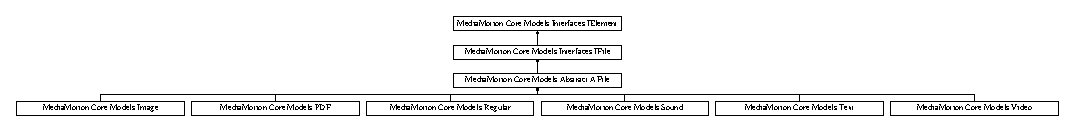
\includegraphics[height=1.328588cm]{class_media_motion_1_1_core_1_1_models_1_1_abstract_1_1_a_file}
\end{center}
\end{figure}
\subsection*{Public Member Functions}
\begin{DoxyCompactItemize}
\item 
\hypertarget{class_media_motion_1_1_core_1_1_models_1_1_abstract_1_1_a_file_a5301a4dd52ccbaf6a2185c407871f51e}{Element\+Type {\bfseries get\+Element\+Type} ()}\label{class_media_motion_1_1_core_1_1_models_1_1_abstract_1_1_a_file_a5301a4dd52ccbaf6a2185c407871f51e}

\item 
\hypertarget{class_media_motion_1_1_core_1_1_models_1_1_abstract_1_1_a_file_a9c2c24170fe743b1ab0042f02687b090}{File\+Type {\bfseries get\+File\+Type} ()}\label{class_media_motion_1_1_core_1_1_models_1_1_abstract_1_1_a_file_a9c2c24170fe743b1ab0042f02687b090}

\end{DoxyCompactItemize}
\subsection*{Protected Attributes}
\begin{DoxyCompactItemize}
\item 
\hypertarget{class_media_motion_1_1_core_1_1_models_1_1_abstract_1_1_a_file_a44655451e9d959d2348ca0f6317da796}{File\+Type {\bfseries file\+Type}}\label{class_media_motion_1_1_core_1_1_models_1_1_abstract_1_1_a_file_a44655451e9d959d2348ca0f6317da796}

\end{DoxyCompactItemize}


The documentation for this class was generated from the following file\+:\begin{DoxyCompactItemize}
\item 
O\+:/\+Projects/\+Media\+Motion/\+Media\+Motion/\+Assets/\+Scripts/\+Core/\+Models/\+File\+Manager/\+Abstracts/A\+File.\+cs\end{DoxyCompactItemize}

\hypertarget{class_media_motion_1_1_modules_1_1_media_player_1_1_a_media_player}{\section{Media\+Motion.\+Modules.\+Media\+Player.\+A\+Media\+Player Class Reference}
\label{class_media_motion_1_1_modules_1_1_media_player_1_1_a_media_player}\index{Media\+Motion.\+Modules.\+Media\+Player.\+A\+Media\+Player@{Media\+Motion.\+Modules.\+Media\+Player.\+A\+Media\+Player}}
}
Inheritance diagram for Media\+Motion.\+Modules.\+Media\+Player.\+A\+Media\+Player\+:\begin{figure}[H]
\begin{center}
\leavevmode
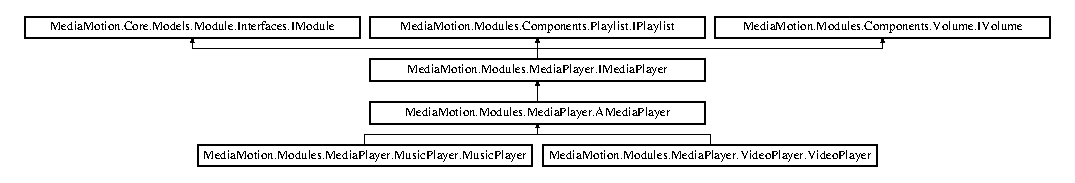
\includegraphics[height=2.012578cm]{class_media_motion_1_1_modules_1_1_media_player_1_1_a_media_player}
\end{center}
\end{figure}
\subsection*{Public Member Functions}
\begin{DoxyCompactItemize}
\item 
\hypertarget{class_media_motion_1_1_modules_1_1_media_player_1_1_a_media_player_a152a3352c27602e3a3305390bcc16fe6}{delegate void {\bfseries Media\+Handle} (object sender, \hyperlink{class_media_motion_1_1_modules_1_1_media_player_1_1_events_1_1_media_event_args}{Media\+Event\+Args} e)}\label{class_media_motion_1_1_modules_1_1_media_player_1_1_a_media_player_a152a3352c27602e3a3305390bcc16fe6}

\item 
\hypertarget{class_media_motion_1_1_modules_1_1_media_player_1_1_a_media_player_a35d6aea691f8ba6365f684c5865842d9}{void {\bfseries Play} ()}\label{class_media_motion_1_1_modules_1_1_media_player_1_1_a_media_player_a35d6aea691f8ba6365f684c5865842d9}

\item 
\hypertarget{class_media_motion_1_1_modules_1_1_media_player_1_1_a_media_player_aeebef99202d3ac2f833f519c09c71c0d}{void {\bfseries Pause} ()}\label{class_media_motion_1_1_modules_1_1_media_player_1_1_a_media_player_aeebef99202d3ac2f833f519c09c71c0d}

\item 
\hypertarget{class_media_motion_1_1_modules_1_1_media_player_1_1_a_media_player_a45bb4d272b2022559e61210034ddc78e}{void {\bfseries Stop} ()}\label{class_media_motion_1_1_modules_1_1_media_player_1_1_a_media_player_a45bb4d272b2022559e61210034ddc78e}

\item 
\hypertarget{class_media_motion_1_1_modules_1_1_media_player_1_1_a_media_player_a820d9a90f7091a20ec57621be67880fa}{\hyperlink{interface_media_motion_1_1_core_1_1_models_1_1_interfaces_1_1_i_element}{I\+Element} {\bfseries Current} ()}\label{class_media_motion_1_1_modules_1_1_media_player_1_1_a_media_player_a820d9a90f7091a20ec57621be67880fa}

\item 
\hypertarget{class_media_motion_1_1_modules_1_1_media_player_1_1_a_media_player_acddad4e17eee316ca8550df77b17a7e5}{void {\bfseries Prev} ()}\label{class_media_motion_1_1_modules_1_1_media_player_1_1_a_media_player_acddad4e17eee316ca8550df77b17a7e5}

\item 
\hypertarget{class_media_motion_1_1_modules_1_1_media_player_1_1_a_media_player_a0471286e48a8708a6128f0677323ee34}{void {\bfseries Next} ()}\label{class_media_motion_1_1_modules_1_1_media_player_1_1_a_media_player_a0471286e48a8708a6128f0677323ee34}

\item 
\hypertarget{class_media_motion_1_1_modules_1_1_media_player_1_1_a_media_player_aff076e87c0434d3ac354179df24c4983}{void {\bfseries Add} (List$<$ \hyperlink{interface_media_motion_1_1_core_1_1_models_1_1_interfaces_1_1_i_element}{I\+Element} $>$ Elements)}\label{class_media_motion_1_1_modules_1_1_media_player_1_1_a_media_player_aff076e87c0434d3ac354179df24c4983}

\item 
\hypertarget{class_media_motion_1_1_modules_1_1_media_player_1_1_a_media_player_a99d62c41fda798cae04bdfd07aa69fa5}{void {\bfseries Remove} (List$<$ \hyperlink{interface_media_motion_1_1_core_1_1_models_1_1_interfaces_1_1_i_element}{I\+Element} $>$ Elements)}\label{class_media_motion_1_1_modules_1_1_media_player_1_1_a_media_player_a99d62c41fda798cae04bdfd07aa69fa5}

\item 
\hypertarget{class_media_motion_1_1_modules_1_1_media_player_1_1_a_media_player_a48d64ea14b422a16714343f5b792a9ea}{void {\bfseries Volume\+Up} ()}\label{class_media_motion_1_1_modules_1_1_media_player_1_1_a_media_player_a48d64ea14b422a16714343f5b792a9ea}

\item 
\hypertarget{class_media_motion_1_1_modules_1_1_media_player_1_1_a_media_player_a251cebc54b2eff4d097b5c281334e51d}{void {\bfseries Volume\+Down} ()}\label{class_media_motion_1_1_modules_1_1_media_player_1_1_a_media_player_a251cebc54b2eff4d097b5c281334e51d}

\end{DoxyCompactItemize}
\subsection*{Protected Attributes}
\begin{DoxyCompactItemize}
\item 
\hypertarget{class_media_motion_1_1_modules_1_1_media_player_1_1_a_media_player_a7665ae887e627d205d70aebba59f58eb}{\hyperlink{class_media_motion_1_1_modules_1_1_components_1_1_playlist_1_1_playlist}{Playlist} {\bfseries Playlist}}\label{class_media_motion_1_1_modules_1_1_media_player_1_1_a_media_player_a7665ae887e627d205d70aebba59f58eb}

\item 
\hypertarget{class_media_motion_1_1_modules_1_1_media_player_1_1_a_media_player_a6f5dd174fcedcba77cf9c79fd4c4dc0b}{\hyperlink{class_media_motion_1_1_modules_1_1_components_1_1_volume_1_1_volume}{Volume} {\bfseries Volume}}\label{class_media_motion_1_1_modules_1_1_media_player_1_1_a_media_player_a6f5dd174fcedcba77cf9c79fd4c4dc0b}

\end{DoxyCompactItemize}
\subsection*{Properties}
\begin{DoxyCompactItemize}
\item 
\hypertarget{class_media_motion_1_1_modules_1_1_media_player_1_1_a_media_player_a29ac1f7c962118ba34d461799f00eeda}{bool {\bfseries Random}\hspace{0.3cm}{\ttfamily  \mbox{[}get, set\mbox{]}}}\label{class_media_motion_1_1_modules_1_1_media_player_1_1_a_media_player_a29ac1f7c962118ba34d461799f00eeda}

\item 
\hypertarget{class_media_motion_1_1_modules_1_1_media_player_1_1_a_media_player_a28fb72902ee85e50daa7f303b46853e2}{bool {\bfseries Loop}\hspace{0.3cm}{\ttfamily  \mbox{[}get, set\mbox{]}}}\label{class_media_motion_1_1_modules_1_1_media_player_1_1_a_media_player_a28fb72902ee85e50daa7f303b46853e2}

\item 
\hypertarget{class_media_motion_1_1_modules_1_1_media_player_1_1_a_media_player_a79267fda4e4d4507cb22afa0df1d5eef}{int {\bfseries Sound}\hspace{0.3cm}{\ttfamily  \mbox{[}get\mbox{]}}}\label{class_media_motion_1_1_modules_1_1_media_player_1_1_a_media_player_a79267fda4e4d4507cb22afa0df1d5eef}

\item 
\hypertarget{class_media_motion_1_1_modules_1_1_media_player_1_1_a_media_player_ae7ee002fc13e1564ec66fec4b941caf6}{int {\bfseries Step}\hspace{0.3cm}{\ttfamily  \mbox{[}get\mbox{]}}}\label{class_media_motion_1_1_modules_1_1_media_player_1_1_a_media_player_ae7ee002fc13e1564ec66fec4b941caf6}

\item 
\hypertarget{class_media_motion_1_1_modules_1_1_media_player_1_1_a_media_player_a607976f0c627f55c3d37662c61b669ee}{Playlist.\+Playlist\+Element\+Change\+Handler {\bfseries On\+Element\+Change}}\label{class_media_motion_1_1_modules_1_1_media_player_1_1_a_media_player_a607976f0c627f55c3d37662c61b669ee}

\item 
\hypertarget{class_media_motion_1_1_modules_1_1_media_player_1_1_a_media_player_a65d514d22afc077898c88e0e3c7c6913}{Playlist.\+Playlist\+Change\+Handler {\bfseries On\+Playlist\+Change}}\label{class_media_motion_1_1_modules_1_1_media_player_1_1_a_media_player_a65d514d22afc077898c88e0e3c7c6913}

\item 
\hypertarget{class_media_motion_1_1_modules_1_1_media_player_1_1_a_media_player_a1f77dbd1006da4cd3356de2cfdcc674e}{Volume.\+Volume\+Change\+Handler {\bfseries On\+Volume\+Change}}\label{class_media_motion_1_1_modules_1_1_media_player_1_1_a_media_player_a1f77dbd1006da4cd3356de2cfdcc674e}

\end{DoxyCompactItemize}
\subsection*{Events}
\begin{DoxyCompactItemize}
\item 
\hypertarget{class_media_motion_1_1_modules_1_1_media_player_1_1_a_media_player_aaebbdcf185860af282d28b9b794715a8}{Media\+Handle {\bfseries On\+Play}}\label{class_media_motion_1_1_modules_1_1_media_player_1_1_a_media_player_aaebbdcf185860af282d28b9b794715a8}

\item 
\hypertarget{class_media_motion_1_1_modules_1_1_media_player_1_1_a_media_player_ada53a81f988f6417fbc164f2d127c7c0}{Media\+Handle {\bfseries On\+Pause}}\label{class_media_motion_1_1_modules_1_1_media_player_1_1_a_media_player_ada53a81f988f6417fbc164f2d127c7c0}

\item 
\hypertarget{class_media_motion_1_1_modules_1_1_media_player_1_1_a_media_player_a736b75fe807f3e553281ae7f9a1bf44d}{Media\+Handle {\bfseries On\+Stop}}\label{class_media_motion_1_1_modules_1_1_media_player_1_1_a_media_player_a736b75fe807f3e553281ae7f9a1bf44d}

\end{DoxyCompactItemize}


The documentation for this class was generated from the following file\+:\begin{DoxyCompactItemize}
\item 
O\+:/\+Projects/\+Media\+Motion/\+Media\+Motion/\+Assets/\+Scripts/\+Modules/\+Media\+Player/A\+Media\+Player.\+cs\end{DoxyCompactItemize}

\hypertarget{class_element_u_i}{\section{Element\+U\+I Class Reference}
\label{class_element_u_i}\index{Element\+U\+I@{Element\+U\+I}}
}
Inheritance diagram for Element\+U\+I\+:\begin{figure}[H]
\begin{center}
\leavevmode
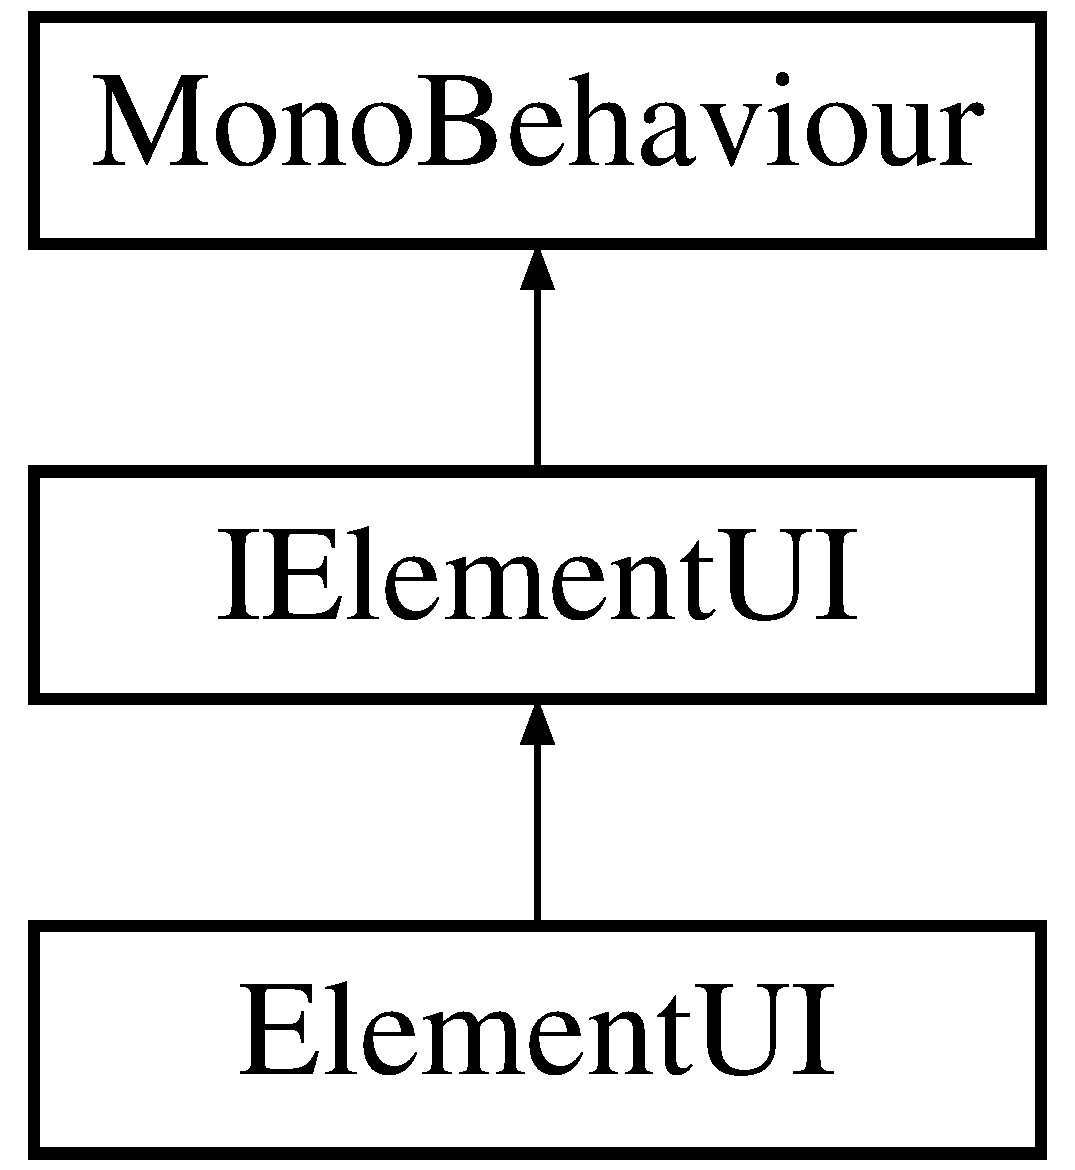
\includegraphics[height=3.000000cm]{class_element_u_i}
\end{center}
\end{figure}
\subsection*{Additional Inherited Members}


The documentation for this class was generated from the following file\+:\begin{DoxyCompactItemize}
\item 
O\+:/\+Projects/\+Media\+Motion/\+Media\+Motion/\+Assets/\+Scripts/\+Core/\+View/Element\+U\+I.\+cs\end{DoxyCompactItemize}

\hypertarget{class_file_u_i}{\section{File\+U\+I Class Reference}
\label{class_file_u_i}\index{File\+U\+I@{File\+U\+I}}
}
Inheritance diagram for File\+U\+I\+:\begin{figure}[H]
\begin{center}
\leavevmode
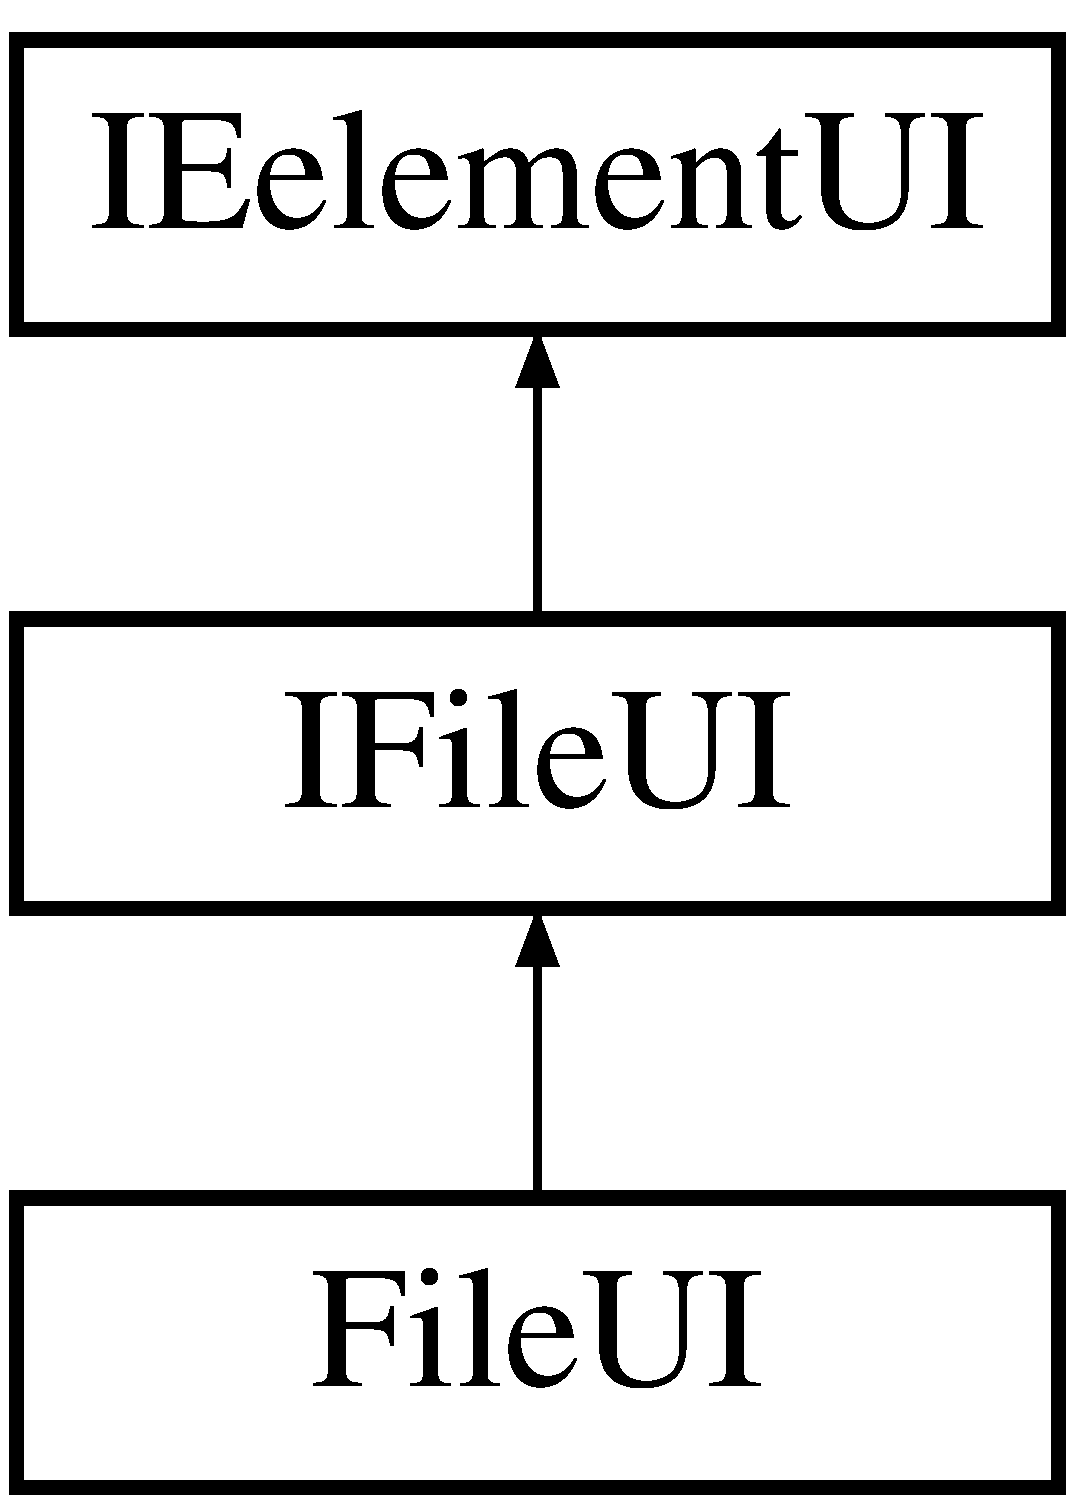
\includegraphics[height=3.000000cm]{class_file_u_i}
\end{center}
\end{figure}
\subsection*{Additional Inherited Members}


The documentation for this class was generated from the following file\+:\begin{DoxyCompactItemize}
\item 
O\+:/\+Projects/\+Media\+Motion/\+Media\+Motion/\+Assets/\+Scripts/\+Core/\+View/File\+U\+I.\+cs\end{DoxyCompactItemize}

\hypertarget{class_media_motion_1_1_core_1_1_controllers_1_1_folder_content_controller}{\section{Media\+Motion.\+Core.\+Controllers.\+Folder\+Content\+Controller Class Reference}
\label{class_media_motion_1_1_core_1_1_controllers_1_1_folder_content_controller}\index{Media\+Motion.\+Core.\+Controllers.\+Folder\+Content\+Controller@{Media\+Motion.\+Core.\+Controllers.\+Folder\+Content\+Controller}}
}
Inheritance diagram for Media\+Motion.\+Core.\+Controllers.\+Folder\+Content\+Controller\+:\begin{figure}[H]
\begin{center}
\leavevmode
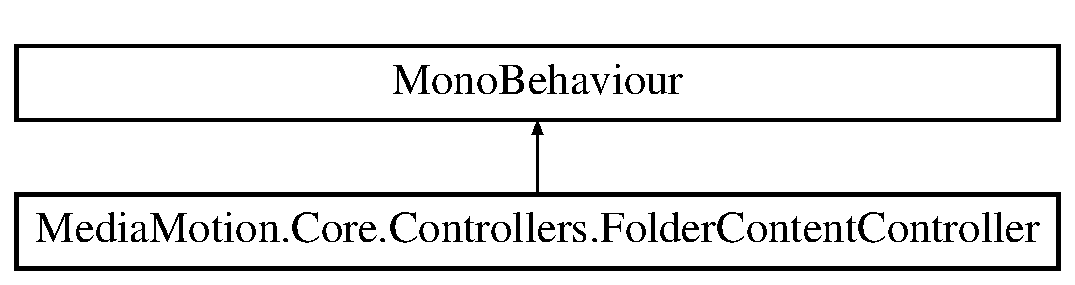
\includegraphics[height=2.000000cm]{class_media_motion_1_1_core_1_1_controllers_1_1_folder_content_controller}
\end{center}
\end{figure}


The documentation for this class was generated from the following file\+:\begin{DoxyCompactItemize}
\item 
O\+:/\+Projects/\+Media\+Motion/\+Media\+Motion/\+Assets/\+Scripts/\+Core/\+Controllers/Folder\+Content\+Controller.\+cs\end{DoxyCompactItemize}

\hypertarget{class_folder_content_u_i}{\section{Folder\+Content\+U\+I Class Reference}
\label{class_folder_content_u_i}\index{Folder\+Content\+U\+I@{Folder\+Content\+U\+I}}
}
Inheritance diagram for Folder\+Content\+U\+I\+:\begin{figure}[H]
\begin{center}
\leavevmode
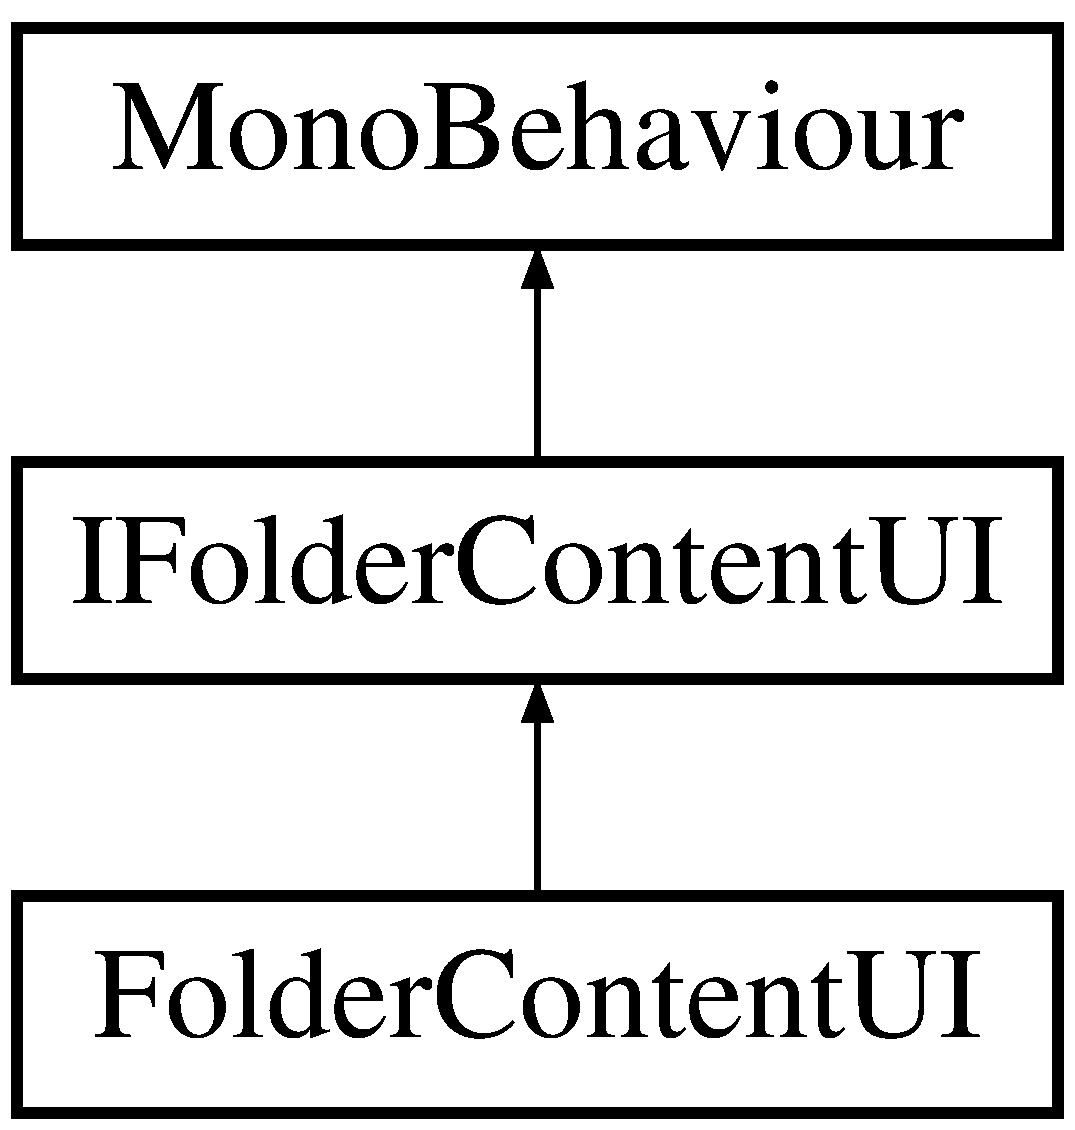
\includegraphics[height=3.000000cm]{class_folder_content_u_i}
\end{center}
\end{figure}
\subsection*{Additional Inherited Members}


The documentation for this class was generated from the following file\+:\begin{DoxyCompactItemize}
\item 
O\+:/\+Projects/\+Media\+Motion/\+Media\+Motion/\+Assets/\+Scripts/\+Core/\+View/Folder\+Content\+U\+I.\+cs\end{DoxyCompactItemize}

\hypertarget{class_folder_u_i}{\section{Folder\+U\+I Class Reference}
\label{class_folder_u_i}\index{Folder\+U\+I@{Folder\+U\+I}}
}
Inheritance diagram for Folder\+U\+I\+:\begin{figure}[H]
\begin{center}
\leavevmode
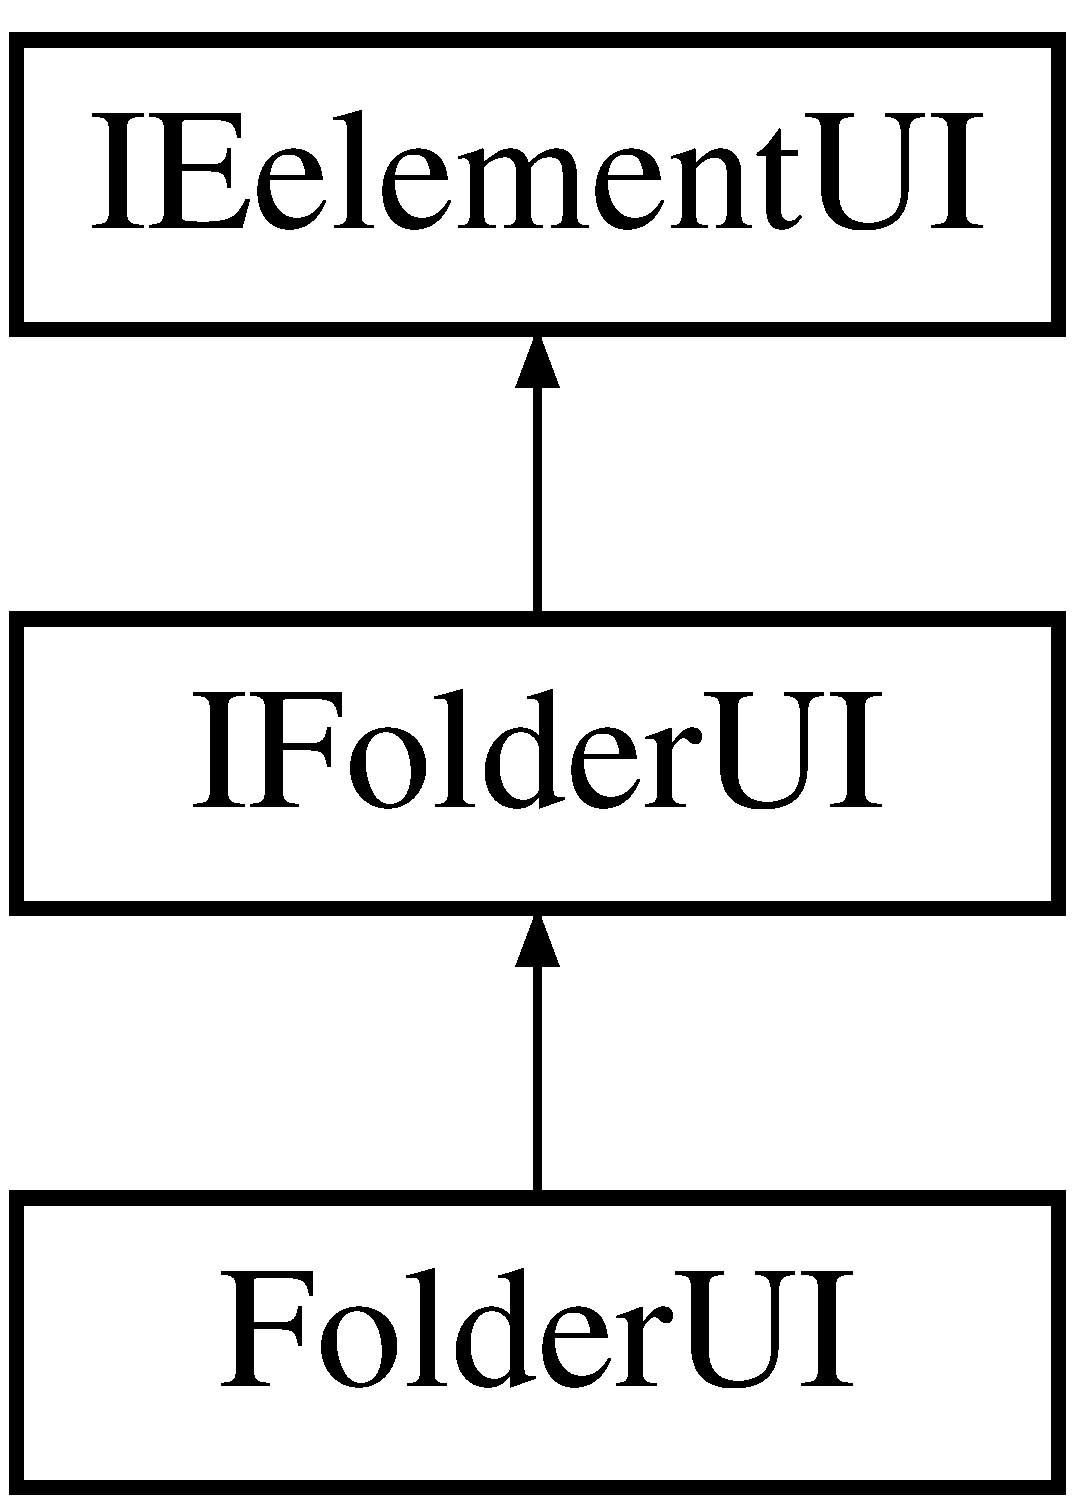
\includegraphics[height=3.000000cm]{class_folder_u_i}
\end{center}
\end{figure}
\subsection*{Additional Inherited Members}


The documentation for this class was generated from the following file\+:\begin{DoxyCompactItemize}
\item 
O\+:/\+Projects/\+Media\+Motion/\+Media\+Motion/\+Assets/\+Scripts/\+Core/\+View/Folder\+U\+I.\+cs\end{DoxyCompactItemize}

\hypertarget{interface_media_motion_1_1_core_1_1_models_1_1_interfaces_1_1_i_element}{\section{Media\+Motion.\+Core.\+Models.\+Interfaces.\+I\+Element Interface Reference}
\label{interface_media_motion_1_1_core_1_1_models_1_1_interfaces_1_1_i_element}\index{Media\+Motion.\+Core.\+Models.\+Interfaces.\+I\+Element@{Media\+Motion.\+Core.\+Models.\+Interfaces.\+I\+Element}}
}
Inheritance diagram for Media\+Motion.\+Core.\+Models.\+Interfaces.\+I\+Element\+:\begin{figure}[H]
\begin{center}
\leavevmode
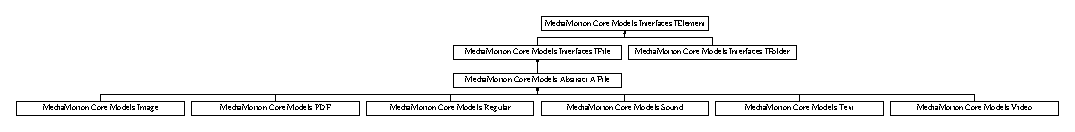
\includegraphics[height=1.328588cm]{interface_media_motion_1_1_core_1_1_models_1_1_interfaces_1_1_i_element}
\end{center}
\end{figure}
\subsection*{Public Member Functions}
\begin{DoxyCompactItemize}
\item 
\hypertarget{interface_media_motion_1_1_core_1_1_models_1_1_interfaces_1_1_i_element_a0cb02a2f042b8c70ab2cd63937f1219f}{Element\+Type {\bfseries get\+Element\+Type} ()}\label{interface_media_motion_1_1_core_1_1_models_1_1_interfaces_1_1_i_element_a0cb02a2f042b8c70ab2cd63937f1219f}

\end{DoxyCompactItemize}


The documentation for this interface was generated from the following file\+:\begin{DoxyCompactItemize}
\item 
O\+:/\+Projects/\+Media\+Motion/\+Media\+Motion/\+Assets/\+Scripts/\+Core/\+Models/\+File\+Manager/\+Interfaces/I\+Element.\+cs\end{DoxyCompactItemize}

\hypertarget{interface_i_element_u_i}{\section{I\+Element\+U\+I Interface Reference}
\label{interface_i_element_u_i}\index{I\+Element\+U\+I@{I\+Element\+U\+I}}
}
Inheritance diagram for I\+Element\+U\+I\+:\begin{figure}[H]
\begin{center}
\leavevmode
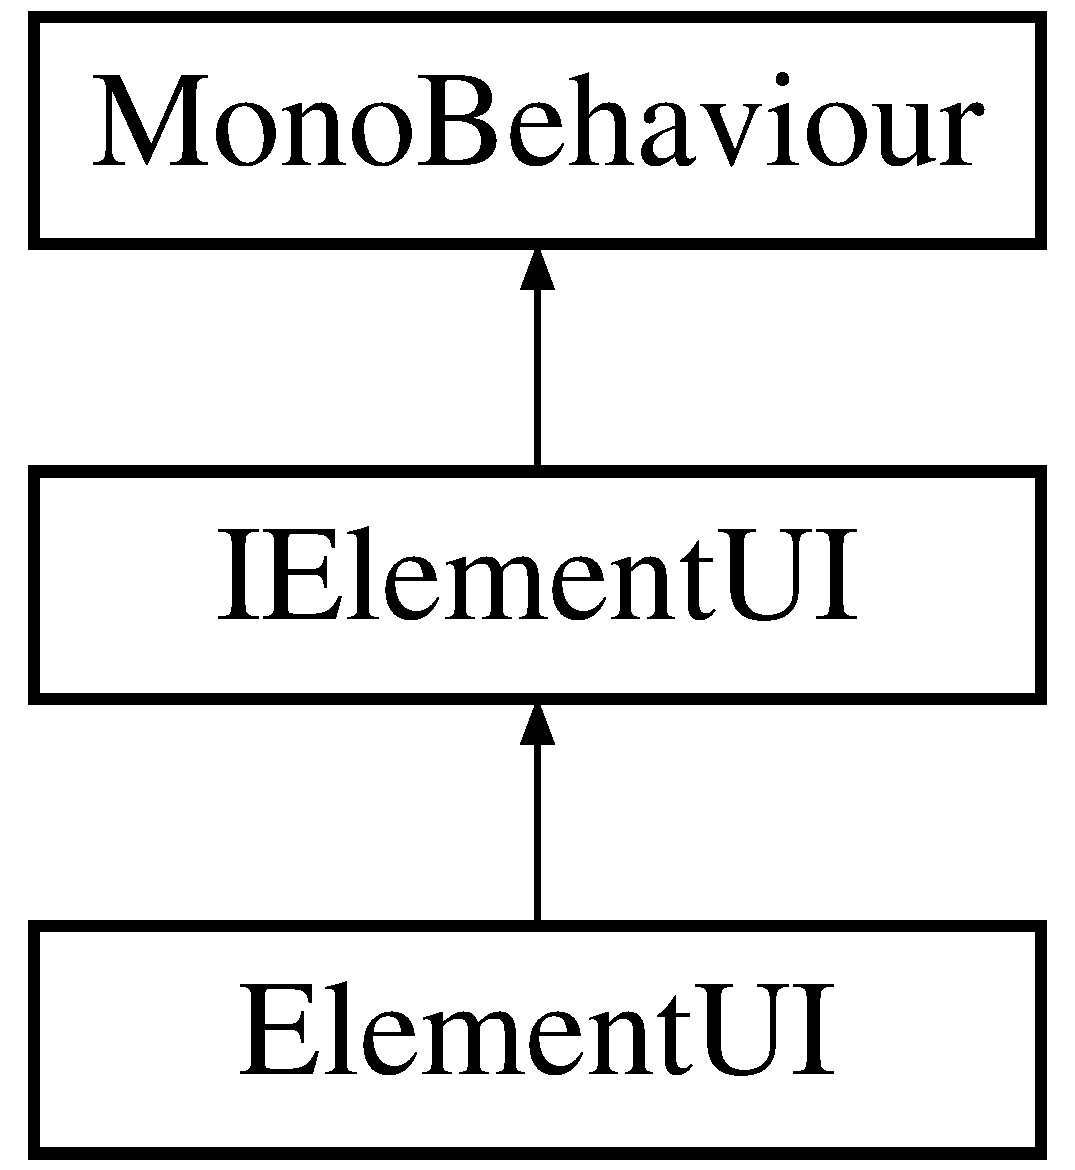
\includegraphics[height=3.000000cm]{interface_i_element_u_i}
\end{center}
\end{figure}
\subsection*{Public Member Functions}
\begin{DoxyCompactItemize}
\item 
\hypertarget{interface_i_element_u_i_a87dece230542967739a62fc5373c2ecd}{void {\bfseries Start} ()}\label{interface_i_element_u_i_a87dece230542967739a62fc5373c2ecd}

\item 
\hypertarget{interface_i_element_u_i_acdbcb4730cdbb571992372f586fd6fed}{void {\bfseries Update} ()}\label{interface_i_element_u_i_acdbcb4730cdbb571992372f586fd6fed}

\end{DoxyCompactItemize}


The documentation for this interface was generated from the following file\+:\begin{DoxyCompactItemize}
\item 
O\+:/\+Projects/\+Media\+Motion/\+Media\+Motion/\+Assets/\+Scripts/\+Core/\+View/\+Interfaces/I\+Element\+U\+I.\+cs\end{DoxyCompactItemize}

\hypertarget{interface_media_motion_1_1_core_1_1_models_1_1_interfaces_1_1_i_file}{\section{Media\+Motion.\+Core.\+Models.\+Interfaces.\+I\+File Interface Reference}
\label{interface_media_motion_1_1_core_1_1_models_1_1_interfaces_1_1_i_file}\index{Media\+Motion.\+Core.\+Models.\+Interfaces.\+I\+File@{Media\+Motion.\+Core.\+Models.\+Interfaces.\+I\+File}}
}
Inheritance diagram for Media\+Motion.\+Core.\+Models.\+Interfaces.\+I\+File\+:\begin{figure}[H]
\begin{center}
\leavevmode
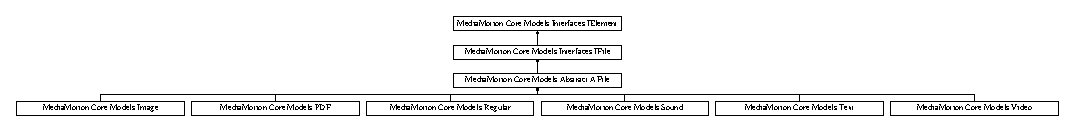
\includegraphics[height=1.328588cm]{interface_media_motion_1_1_core_1_1_models_1_1_interfaces_1_1_i_file}
\end{center}
\end{figure}
\subsection*{Public Member Functions}
\begin{DoxyCompactItemize}
\item 
\hypertarget{interface_media_motion_1_1_core_1_1_models_1_1_interfaces_1_1_i_file_acab39ebbbb6eae529e9413458470d342}{File\+Type {\bfseries get\+File\+Type} ()}\label{interface_media_motion_1_1_core_1_1_models_1_1_interfaces_1_1_i_file_acab39ebbbb6eae529e9413458470d342}

\end{DoxyCompactItemize}


The documentation for this interface was generated from the following file\+:\begin{DoxyCompactItemize}
\item 
O\+:/\+Projects/\+Media\+Motion/\+Media\+Motion/\+Assets/\+Scripts/\+Core/\+Models/\+File\+Manager/\+Interfaces/I\+File.\+cs\end{DoxyCompactItemize}

\hypertarget{interface_i_file_u_i}{\section{I\+File\+U\+I Interface Reference}
\label{interface_i_file_u_i}\index{I\+File\+U\+I@{I\+File\+U\+I}}
}
Inheritance diagram for I\+File\+U\+I\+:\begin{figure}[H]
\begin{center}
\leavevmode
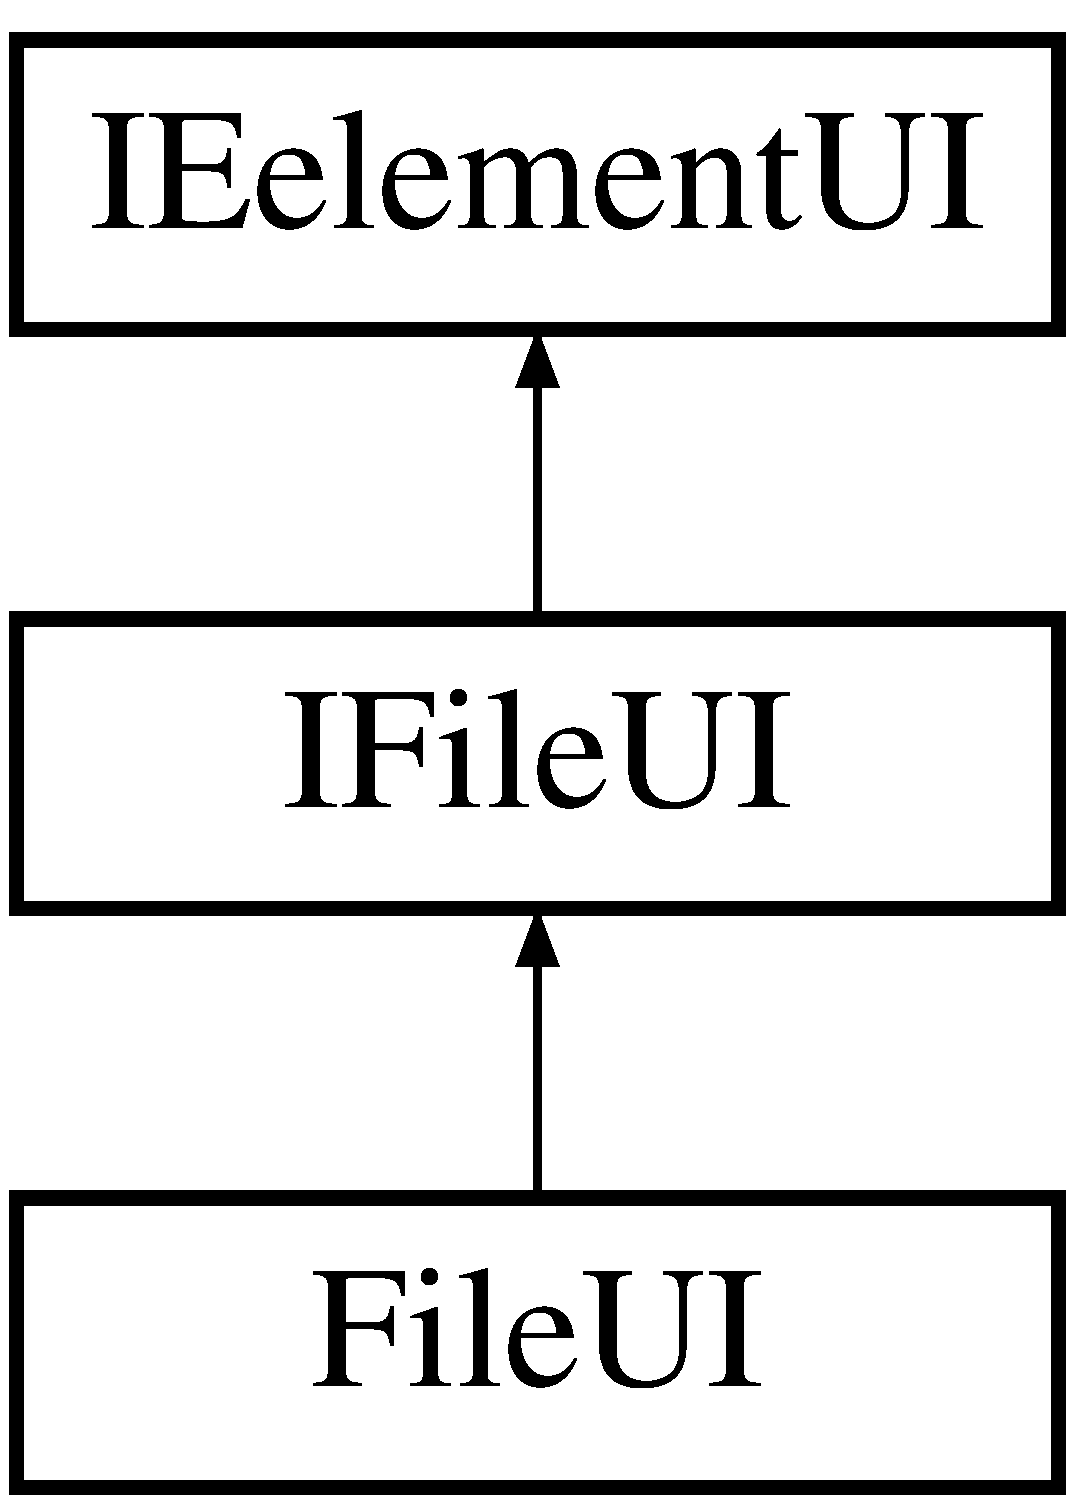
\includegraphics[height=3.000000cm]{interface_i_file_u_i}
\end{center}
\end{figure}
\subsection*{Public Member Functions}
\begin{DoxyCompactItemize}
\item 
\hypertarget{interface_i_file_u_i_a70f1da3b26d079daa1de649de3ebf765}{void {\bfseries Start} ()}\label{interface_i_file_u_i_a70f1da3b26d079daa1de649de3ebf765}

\item 
\hypertarget{interface_i_file_u_i_a0b66b5f236465b5fe7fe3402ea15601a}{void {\bfseries Update} ()}\label{interface_i_file_u_i_a0b66b5f236465b5fe7fe3402ea15601a}

\end{DoxyCompactItemize}


The documentation for this interface was generated from the following file\+:\begin{DoxyCompactItemize}
\item 
O\+:/\+Projects/\+Media\+Motion/\+Media\+Motion/\+Assets/\+Scripts/\+Core/\+View/\+Interfaces/I\+File\+U\+I.\+cs\end{DoxyCompactItemize}

\hypertarget{interface_media_motion_1_1_core_1_1_models_1_1_interfaces_1_1_i_folder}{\section{Media\+Motion.\+Core.\+Models.\+Interfaces.\+I\+Folder Interface Reference}
\label{interface_media_motion_1_1_core_1_1_models_1_1_interfaces_1_1_i_folder}\index{Media\+Motion.\+Core.\+Models.\+Interfaces.\+I\+Folder@{Media\+Motion.\+Core.\+Models.\+Interfaces.\+I\+Folder}}
}
Inheritance diagram for Media\+Motion.\+Core.\+Models.\+Interfaces.\+I\+Folder\+:\begin{figure}[H]
\begin{center}
\leavevmode
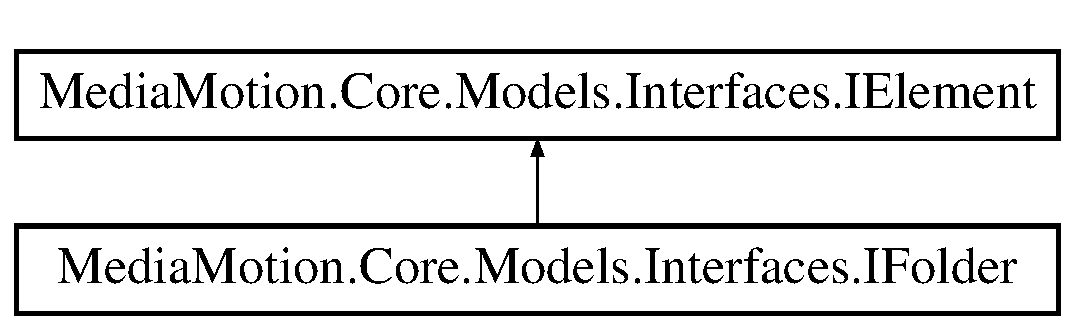
\includegraphics[height=2.000000cm]{interface_media_motion_1_1_core_1_1_models_1_1_interfaces_1_1_i_folder}
\end{center}
\end{figure}
\subsection*{Additional Inherited Members}


The documentation for this interface was generated from the following file\+:\begin{DoxyCompactItemize}
\item 
O\+:/\+Projects/\+Media\+Motion/\+Media\+Motion/\+Assets/\+Scripts/\+Core/\+Models/\+File\+Manager/\+Interfaces/I\+Folder.\+cs\end{DoxyCompactItemize}

\hypertarget{interface_i_folder_content_u_i}{\section{I\+Folder\+Content\+U\+I Interface Reference}
\label{interface_i_folder_content_u_i}\index{I\+Folder\+Content\+U\+I@{I\+Folder\+Content\+U\+I}}
}
Inheritance diagram for I\+Folder\+Content\+U\+I\+:\begin{figure}[H]
\begin{center}
\leavevmode
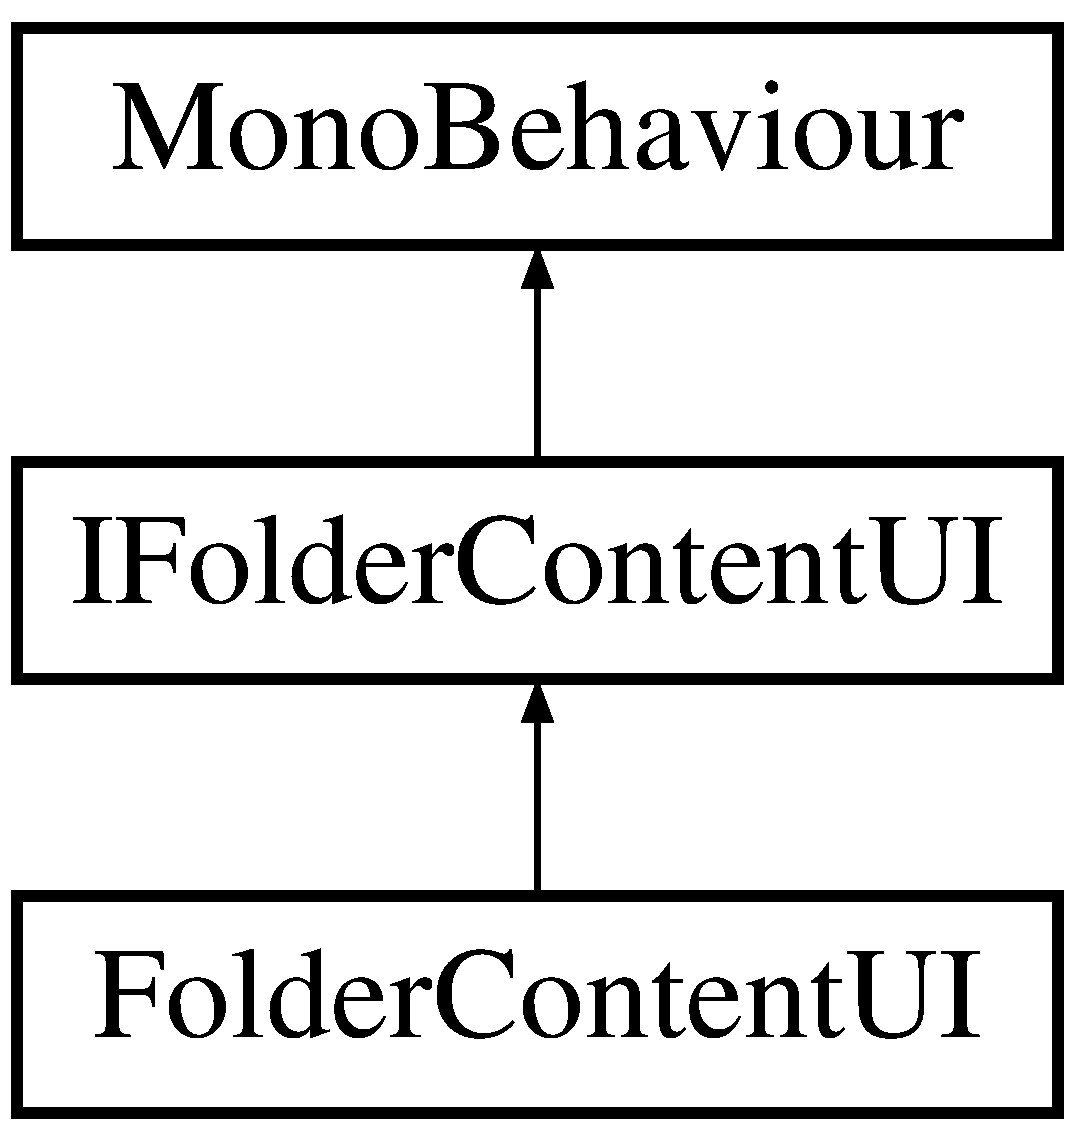
\includegraphics[height=3.000000cm]{interface_i_folder_content_u_i}
\end{center}
\end{figure}
\subsection*{Public Member Functions}
\begin{DoxyCompactItemize}
\item 
\hypertarget{interface_i_folder_content_u_i_a0db9e3fd36e71be958c478729c1fa6b3}{void {\bfseries Start} ()}\label{interface_i_folder_content_u_i_a0db9e3fd36e71be958c478729c1fa6b3}

\item 
\hypertarget{interface_i_folder_content_u_i_a68e74eefabdf59e71c4665b2c5ec6be9}{void {\bfseries Update} ()}\label{interface_i_folder_content_u_i_a68e74eefabdf59e71c4665b2c5ec6be9}

\end{DoxyCompactItemize}


The documentation for this interface was generated from the following file\+:\begin{DoxyCompactItemize}
\item 
O\+:/\+Projects/\+Media\+Motion/\+Media\+Motion/\+Assets/\+Scripts/\+Core/\+View/\+Interfaces/I\+Folder\+Content\+U\+I.\+cs\end{DoxyCompactItemize}

\hypertarget{interface_i_folder_u_i}{\section{I\+Folder\+U\+I Interface Reference}
\label{interface_i_folder_u_i}\index{I\+Folder\+U\+I@{I\+Folder\+U\+I}}
}
Inheritance diagram for I\+Folder\+U\+I\+:\begin{figure}[H]
\begin{center}
\leavevmode
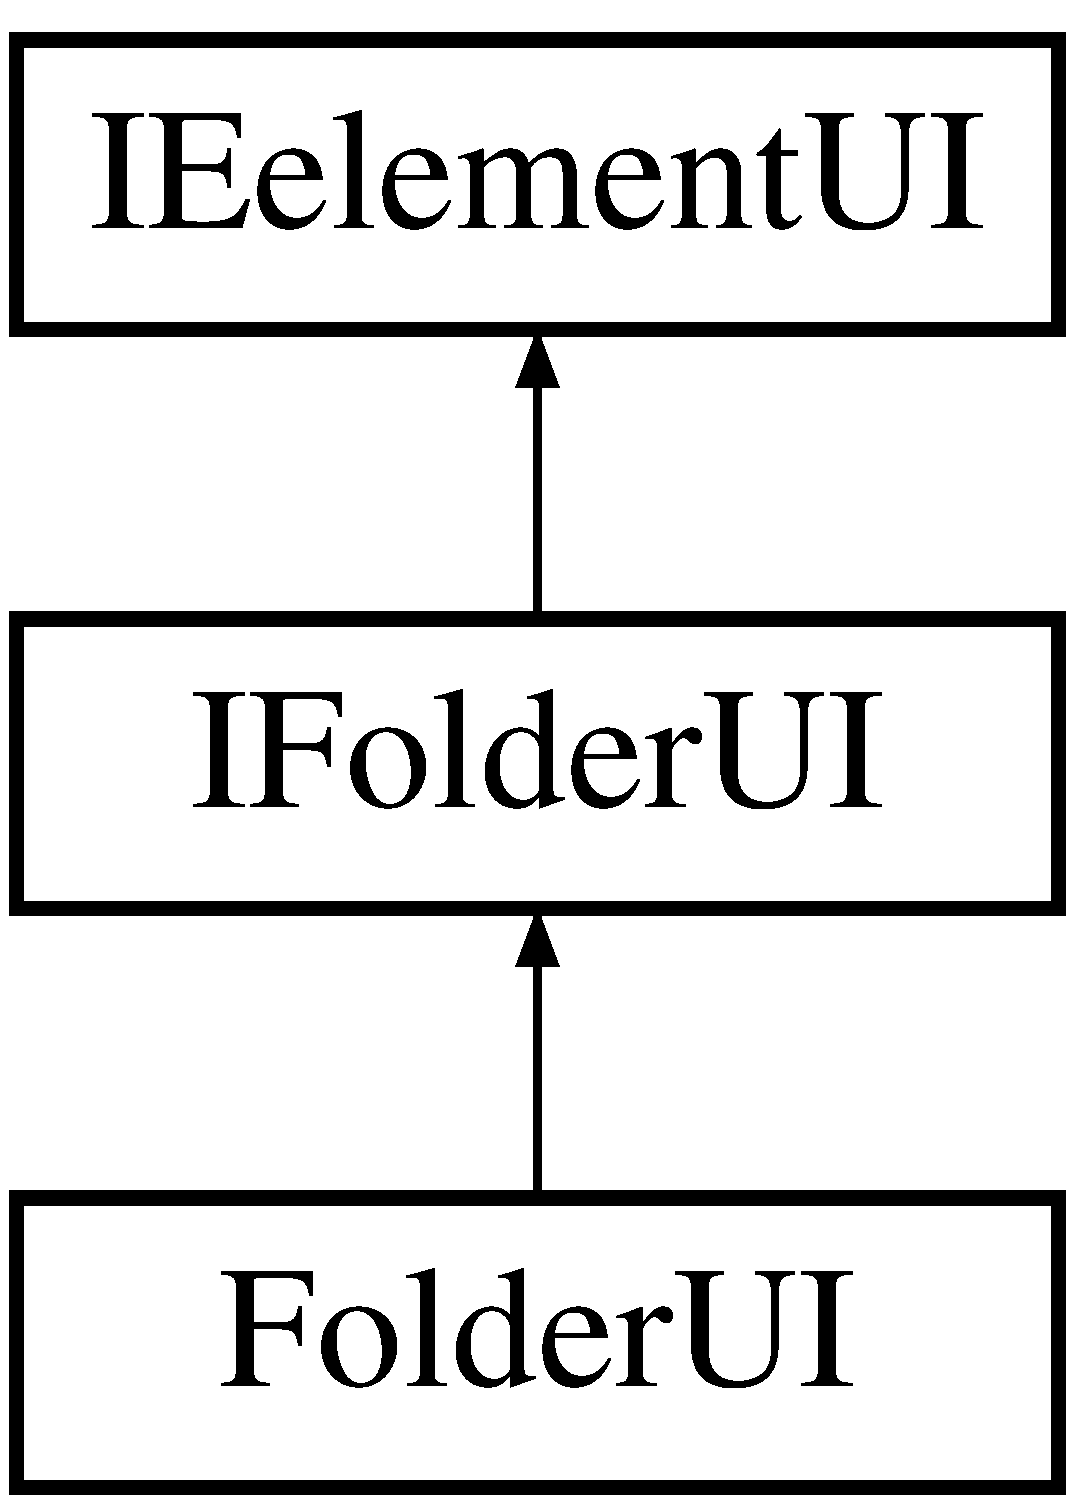
\includegraphics[height=3.000000cm]{interface_i_folder_u_i}
\end{center}
\end{figure}
\subsection*{Public Member Functions}
\begin{DoxyCompactItemize}
\item 
\hypertarget{interface_i_folder_u_i_a2a1eb0bf1ab713996866a6950bbd395c}{void {\bfseries Start} ()}\label{interface_i_folder_u_i_a2a1eb0bf1ab713996866a6950bbd395c}

\item 
\hypertarget{interface_i_folder_u_i_a7531d45be72de5738e999efdb92d2324}{void {\bfseries Update} ()}\label{interface_i_folder_u_i_a7531d45be72de5738e999efdb92d2324}

\end{DoxyCompactItemize}


The documentation for this interface was generated from the following file\+:\begin{DoxyCompactItemize}
\item 
O\+:/\+Projects/\+Media\+Motion/\+Media\+Motion/\+Assets/\+Scripts/\+Core/\+View/\+Interfaces/I\+Folder\+U\+I.\+cs\end{DoxyCompactItemize}

\hypertarget{interface_media_motion_1_1_modules_1_1_image_viewer_1_1_interfaces_1_1_i_image_viewer}{\section{Media\+Motion.\+Modules.\+Image\+Viewer.\+Interfaces.\+I\+Image\+Viewer Interface Reference}
\label{interface_media_motion_1_1_modules_1_1_image_viewer_1_1_interfaces_1_1_i_image_viewer}\index{Media\+Motion.\+Modules.\+Image\+Viewer.\+Interfaces.\+I\+Image\+Viewer@{Media\+Motion.\+Modules.\+Image\+Viewer.\+Interfaces.\+I\+Image\+Viewer}}
}
Inheritance diagram for Media\+Motion.\+Modules.\+Image\+Viewer.\+Interfaces.\+I\+Image\+Viewer\+:\begin{figure}[H]
\begin{center}
\leavevmode
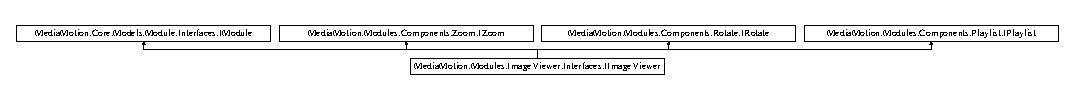
\includegraphics[height=0.773481cm]{interface_media_motion_1_1_modules_1_1_image_viewer_1_1_interfaces_1_1_i_image_viewer}
\end{center}
\end{figure}
\subsection*{Additional Inherited Members}


The documentation for this interface was generated from the following file\+:\begin{DoxyCompactItemize}
\item 
O\+:/\+Projects/\+Media\+Motion/\+Media\+Motion/\+Assets/\+Scripts/\+Modules/\+Image\+Viewer/\+Interfaces/I\+Image\+Viewer.\+cs\end{DoxyCompactItemize}

\hypertarget{interface_i_image_viewer_u_i}{\section{I\+Image\+Viewer\+U\+I Interface Reference}
\label{interface_i_image_viewer_u_i}\index{I\+Image\+Viewer\+U\+I@{I\+Image\+Viewer\+U\+I}}
}
Inheritance diagram for I\+Image\+Viewer\+U\+I\+:\begin{figure}[H]
\begin{center}
\leavevmode
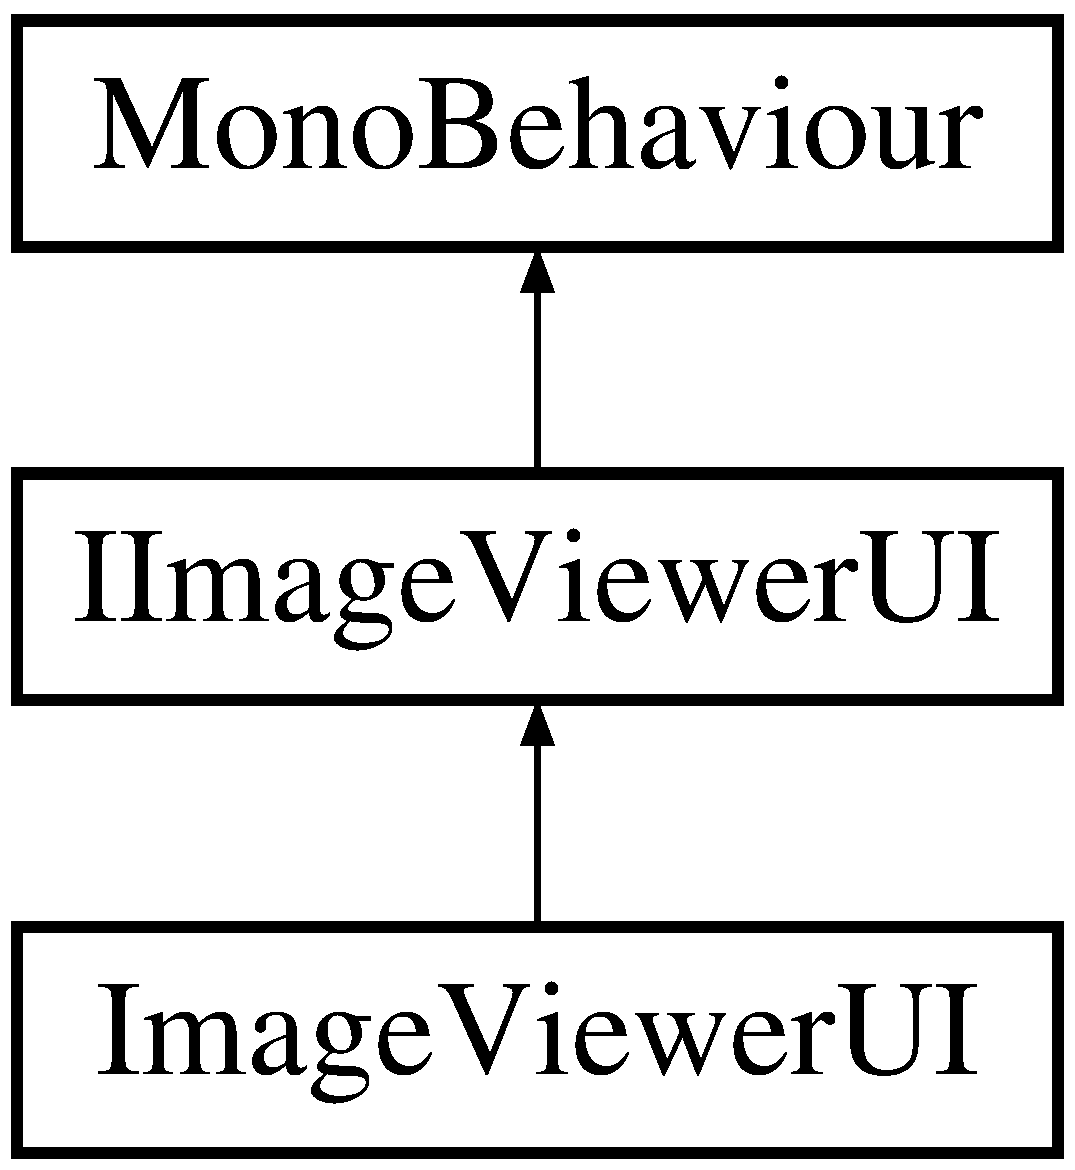
\includegraphics[height=3.000000cm]{interface_i_image_viewer_u_i}
\end{center}
\end{figure}
\subsection*{Public Member Functions}
\begin{DoxyCompactItemize}
\item 
\hypertarget{interface_i_image_viewer_u_i_a5bd01238a79a6a0efb536075817851bb}{void {\bfseries Start} ()}\label{interface_i_image_viewer_u_i_a5bd01238a79a6a0efb536075817851bb}

\item 
\hypertarget{interface_i_image_viewer_u_i_ac21a61f93c1a2b7c04aec352dd6cd715}{void {\bfseries Update} ()}\label{interface_i_image_viewer_u_i_ac21a61f93c1a2b7c04aec352dd6cd715}

\end{DoxyCompactItemize}


The documentation for this interface was generated from the following file\+:\begin{DoxyCompactItemize}
\item 
O\+:/\+Projects/\+Media\+Motion/\+Media\+Motion/\+Assets/\+Scripts/\+Core/\+View/\+Interfaces/I\+Image\+Viewer\+U\+I.\+cs\end{DoxyCompactItemize}

\hypertarget{class_media_motion_1_1_core_1_1_models_1_1_image}{\section{Media\+Motion.\+Core.\+Models.\+Image Class Reference}
\label{class_media_motion_1_1_core_1_1_models_1_1_image}\index{Media\+Motion.\+Core.\+Models.\+Image@{Media\+Motion.\+Core.\+Models.\+Image}}
}
Inheritance diagram for Media\+Motion.\+Core.\+Models.\+Image\+:\begin{figure}[H]
\begin{center}
\leavevmode
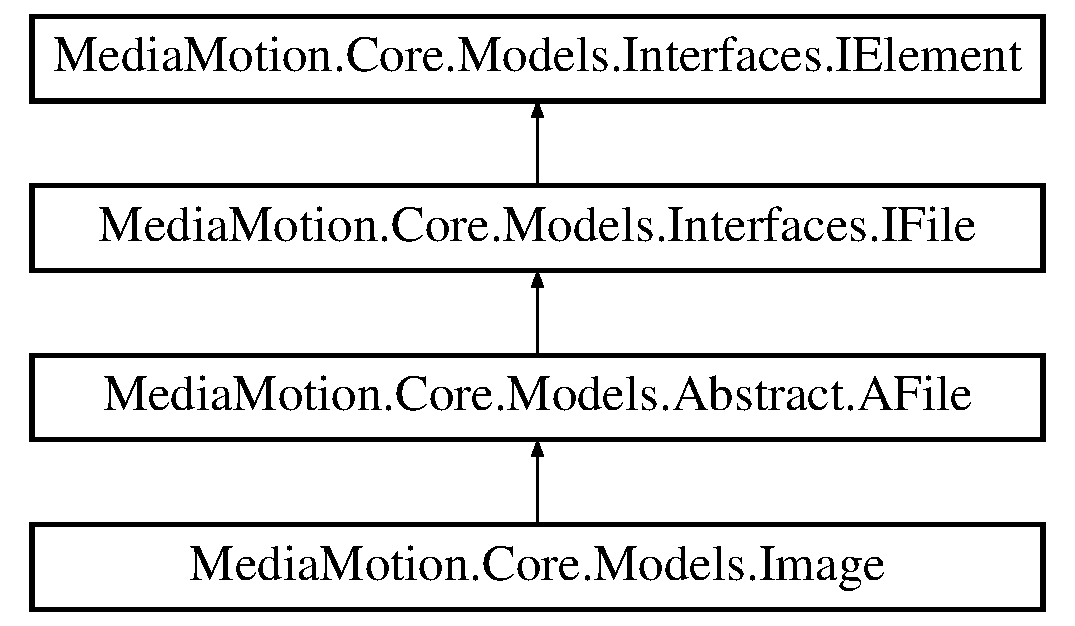
\includegraphics[height=4.000000cm]{class_media_motion_1_1_core_1_1_models_1_1_image}
\end{center}
\end{figure}
\subsection*{Additional Inherited Members}


The documentation for this class was generated from the following file\+:\begin{DoxyCompactItemize}
\item 
O\+:/\+Projects/\+Media\+Motion/\+Media\+Motion/\+Assets/\+Scripts/\+Core/\+Models/\+File\+Manager/Image.\+cs\end{DoxyCompactItemize}

\hypertarget{class_image_viewer_u_i}{\section{Image\+Viewer\+U\+I Class Reference}
\label{class_image_viewer_u_i}\index{Image\+Viewer\+U\+I@{Image\+Viewer\+U\+I}}
}
Inheritance diagram for Image\+Viewer\+U\+I\+:\begin{figure}[H]
\begin{center}
\leavevmode
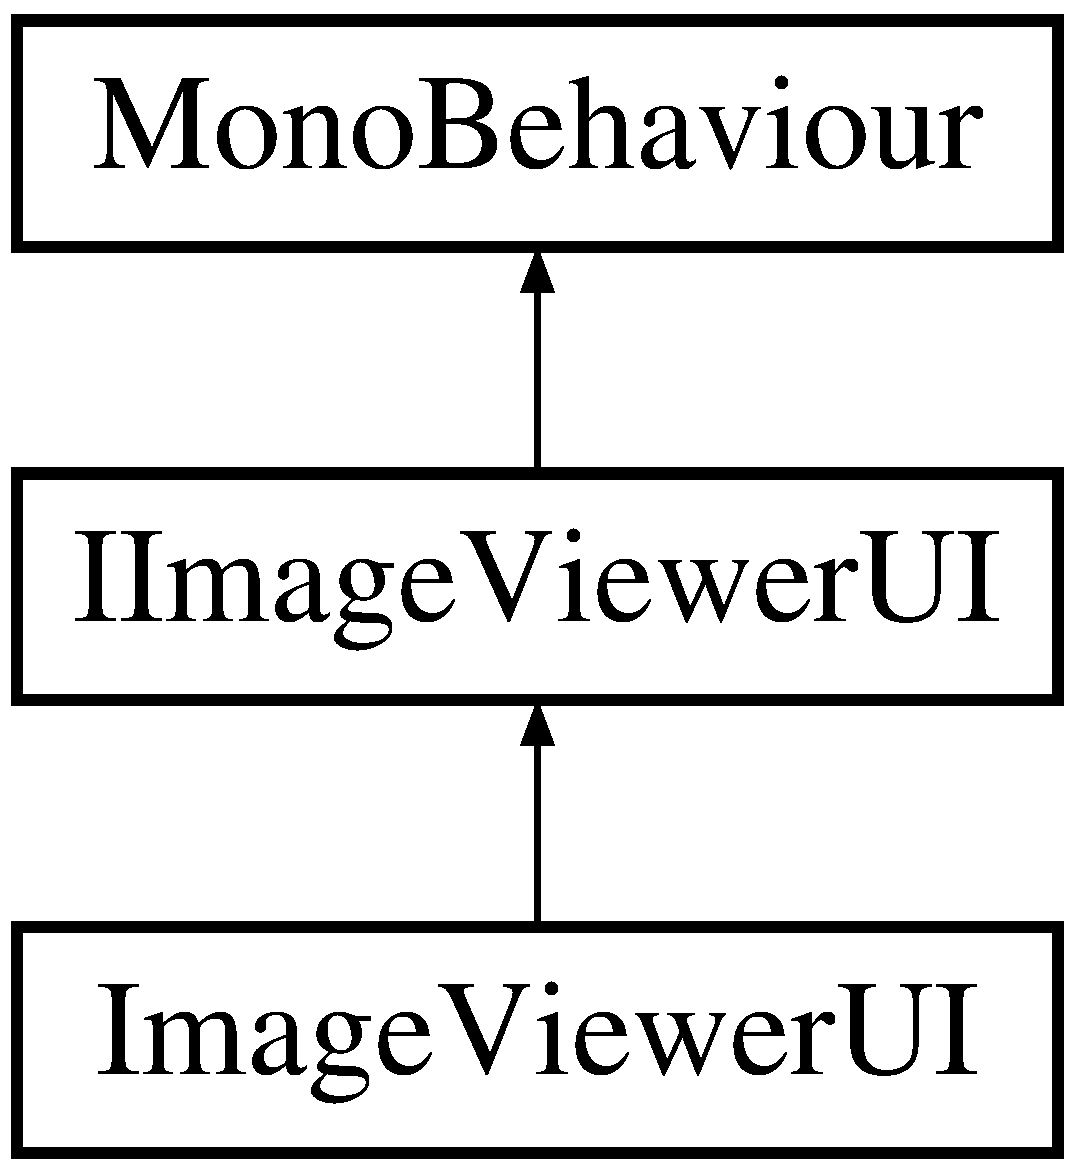
\includegraphics[height=3.000000cm]{class_image_viewer_u_i}
\end{center}
\end{figure}
\subsection*{Additional Inherited Members}


The documentation for this class was generated from the following file\+:\begin{DoxyCompactItemize}
\item 
O\+:/\+Projects/\+Media\+Motion/\+Media\+Motion/\+Assets/\+Scripts/\+Core/\+View/Image\+Viewer\+U\+I.\+cs\end{DoxyCompactItemize}

\hypertarget{interface_media_motion_1_1_modules_1_1_media_player_1_1_i_media_player}{\section{Media\+Motion.\+Modules.\+Media\+Player.\+I\+Media\+Player Interface Reference}
\label{interface_media_motion_1_1_modules_1_1_media_player_1_1_i_media_player}\index{Media\+Motion.\+Modules.\+Media\+Player.\+I\+Media\+Player@{Media\+Motion.\+Modules.\+Media\+Player.\+I\+Media\+Player}}
}
Inheritance diagram for Media\+Motion.\+Modules.\+Media\+Player.\+I\+Media\+Player\+:\begin{figure}[H]
\begin{center}
\leavevmode
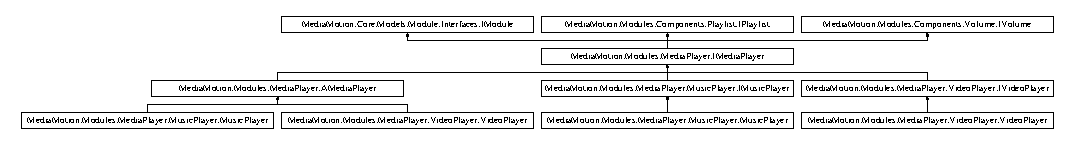
\includegraphics[height=1.497326cm]{interface_media_motion_1_1_modules_1_1_media_player_1_1_i_media_player}
\end{center}
\end{figure}
\subsection*{Public Member Functions}
\begin{DoxyCompactItemize}
\item 
\hypertarget{interface_media_motion_1_1_modules_1_1_media_player_1_1_i_media_player_a12c368634719c16e27feb122122f25c0}{void {\bfseries Play} ()}\label{interface_media_motion_1_1_modules_1_1_media_player_1_1_i_media_player_a12c368634719c16e27feb122122f25c0}

\item 
\hypertarget{interface_media_motion_1_1_modules_1_1_media_player_1_1_i_media_player_a05c231b1472396b15139ceb3ed247681}{void {\bfseries Pause} ()}\label{interface_media_motion_1_1_modules_1_1_media_player_1_1_i_media_player_a05c231b1472396b15139ceb3ed247681}

\item 
\hypertarget{interface_media_motion_1_1_modules_1_1_media_player_1_1_i_media_player_ad77f5fa21bce376e2dd8f9b9068088f6}{void {\bfseries Stop} ()}\label{interface_media_motion_1_1_modules_1_1_media_player_1_1_i_media_player_ad77f5fa21bce376e2dd8f9b9068088f6}

\end{DoxyCompactItemize}
\subsection*{Additional Inherited Members}


The documentation for this interface was generated from the following file\+:\begin{DoxyCompactItemize}
\item 
O\+:/\+Projects/\+Media\+Motion/\+Media\+Motion/\+Assets/\+Scripts/\+Modules/\+Media\+Player/I\+Media\+Player.\+cs\end{DoxyCompactItemize}

\hypertarget{interface_i_media_player_u_i}{\section{I\+Media\+Player\+U\+I Interface Reference}
\label{interface_i_media_player_u_i}\index{I\+Media\+Player\+U\+I@{I\+Media\+Player\+U\+I}}
}
Inheritance diagram for I\+Media\+Player\+U\+I\+:\begin{figure}[H]
\begin{center}
\leavevmode
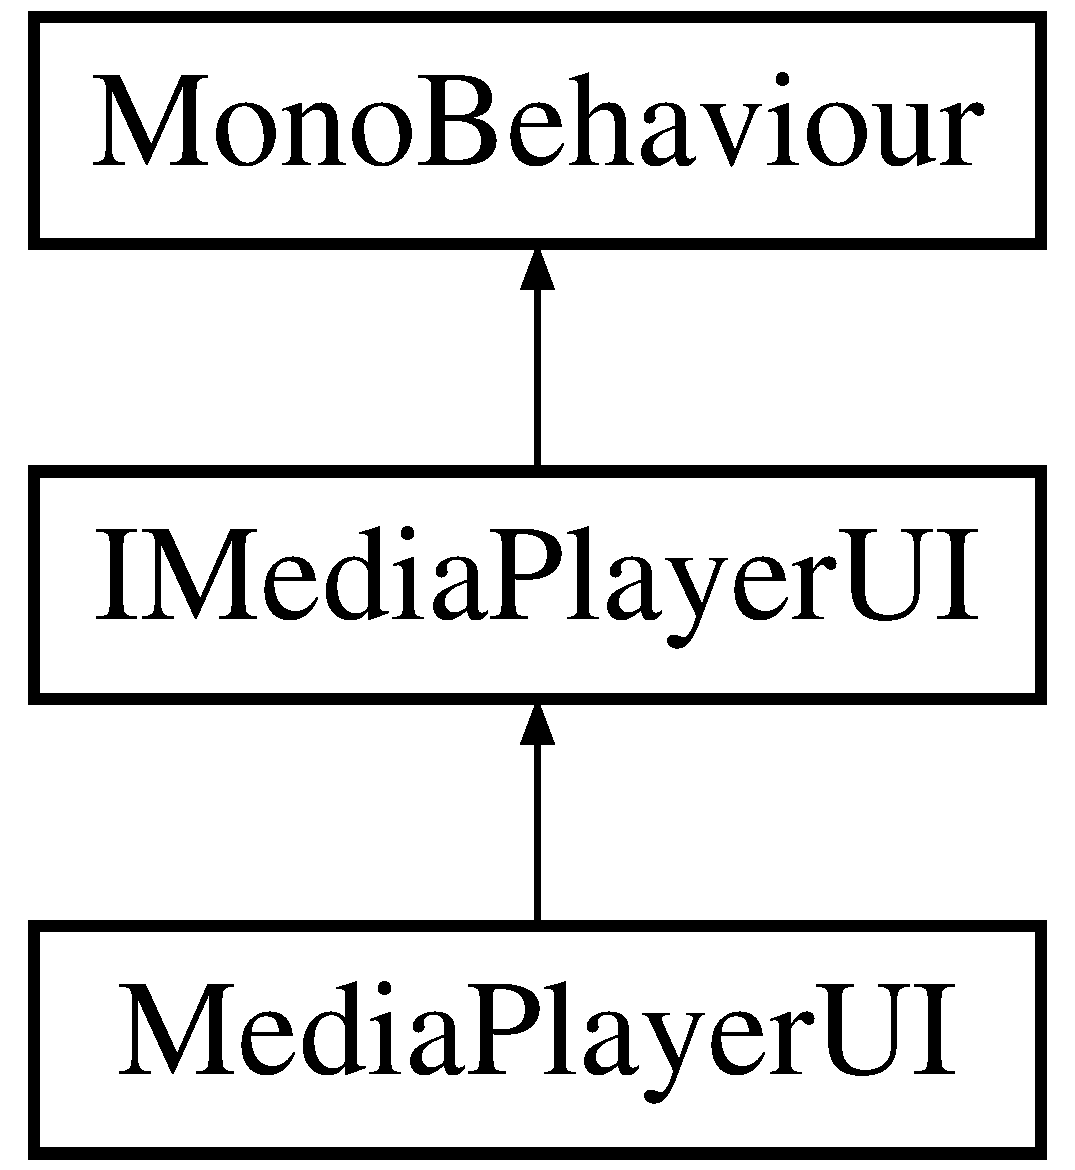
\includegraphics[height=3.000000cm]{interface_i_media_player_u_i}
\end{center}
\end{figure}
\subsection*{Public Member Functions}
\begin{DoxyCompactItemize}
\item 
\hypertarget{interface_i_media_player_u_i_a898b5baebda60dc04aa438d3aabdfd39}{void {\bfseries Start} ()}\label{interface_i_media_player_u_i_a898b5baebda60dc04aa438d3aabdfd39}

\item 
\hypertarget{interface_i_media_player_u_i_a6298eddbf7ac7d81f517c7f4c2e652f7}{void {\bfseries Update} ()}\label{interface_i_media_player_u_i_a6298eddbf7ac7d81f517c7f4c2e652f7}

\end{DoxyCompactItemize}


The documentation for this interface was generated from the following file\+:\begin{DoxyCompactItemize}
\item 
O\+:/\+Projects/\+Media\+Motion/\+Media\+Motion/\+Assets/\+Scripts/\+Core/\+View/\+Interfaces/I\+Media\+Player\+U\+I.\+cs\end{DoxyCompactItemize}

\hypertarget{interface_media_motion_1_1_core_1_1_models_1_1_module_1_1_interfaces_1_1_i_module}{\section{Media\+Motion.\+Core.\+Models.\+Module.\+Interfaces.\+I\+Module Interface Reference}
\label{interface_media_motion_1_1_core_1_1_models_1_1_module_1_1_interfaces_1_1_i_module}\index{Media\+Motion.\+Core.\+Models.\+Module.\+Interfaces.\+I\+Module@{Media\+Motion.\+Core.\+Models.\+Module.\+Interfaces.\+I\+Module}}
}
Inheritance diagram for Media\+Motion.\+Core.\+Models.\+Module.\+Interfaces.\+I\+Module\+:\begin{figure}[H]
\begin{center}
\leavevmode
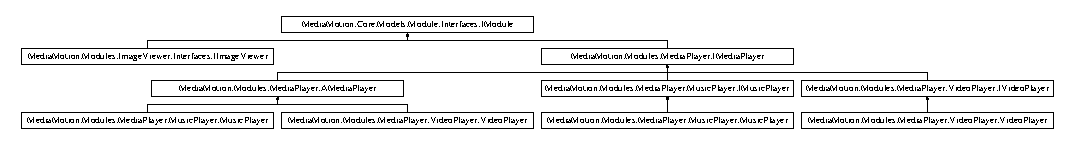
\includegraphics[height=1.497326cm]{interface_media_motion_1_1_core_1_1_models_1_1_module_1_1_interfaces_1_1_i_module}
\end{center}
\end{figure}
\subsection*{Public Member Functions}
\begin{DoxyCompactItemize}
\item 
\hypertarget{interface_media_motion_1_1_core_1_1_models_1_1_module_1_1_interfaces_1_1_i_module_a512dd79360075a410750ca49f12a452d}{void {\bfseries init} ()}\label{interface_media_motion_1_1_core_1_1_models_1_1_module_1_1_interfaces_1_1_i_module_a512dd79360075a410750ca49f12a452d}

\end{DoxyCompactItemize}


The documentation for this interface was generated from the following file\+:\begin{DoxyCompactItemize}
\item 
O\+:/\+Projects/\+Media\+Motion/\+Media\+Motion/\+Assets/\+Scripts/\+Core/\+Models/\+Module/\+Interfaces/I\+Module.\+cs\end{DoxyCompactItemize}

\hypertarget{interface_media_motion_1_1_modules_1_1_media_player_1_1_music_player_1_1_i_music_player}{\section{Media\+Motion.\+Modules.\+Media\+Player.\+Music\+Player.\+I\+Music\+Player Interface Reference}
\label{interface_media_motion_1_1_modules_1_1_media_player_1_1_music_player_1_1_i_music_player}\index{Media\+Motion.\+Modules.\+Media\+Player.\+Music\+Player.\+I\+Music\+Player@{Media\+Motion.\+Modules.\+Media\+Player.\+Music\+Player.\+I\+Music\+Player}}
}
Inheritance diagram for Media\+Motion.\+Modules.\+Media\+Player.\+Music\+Player.\+I\+Music\+Player\+:\begin{figure}[H]
\begin{center}
\leavevmode
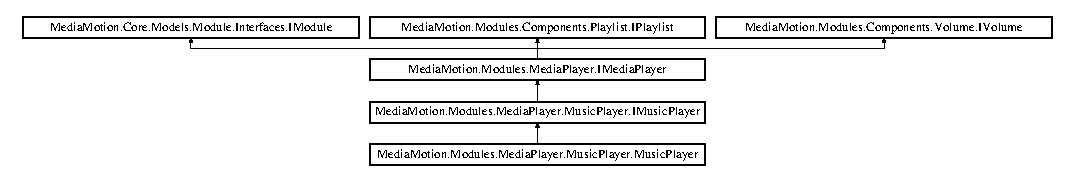
\includegraphics[height=1.996435cm]{interface_media_motion_1_1_modules_1_1_media_player_1_1_music_player_1_1_i_music_player}
\end{center}
\end{figure}
\subsection*{Additional Inherited Members}


The documentation for this interface was generated from the following file\+:\begin{DoxyCompactItemize}
\item 
O\+:/\+Projects/\+Media\+Motion/\+Media\+Motion/\+Assets/\+Scripts/\+Modules/\+Media\+Player/\+Music\+Player/I\+Music\+Player.\+cs\end{DoxyCompactItemize}

\hypertarget{interface_media_motion_1_1_modules_1_1_components_1_1_playlist_1_1_i_playlist}{\section{Media\+Motion.\+Modules.\+Components.\+Playlist.\+I\+Playlist Interface Reference}
\label{interface_media_motion_1_1_modules_1_1_components_1_1_playlist_1_1_i_playlist}\index{Media\+Motion.\+Modules.\+Components.\+Playlist.\+I\+Playlist@{Media\+Motion.\+Modules.\+Components.\+Playlist.\+I\+Playlist}}
}
Inheritance diagram for Media\+Motion.\+Modules.\+Components.\+Playlist.\+I\+Playlist\+:\begin{figure}[H]
\begin{center}
\leavevmode
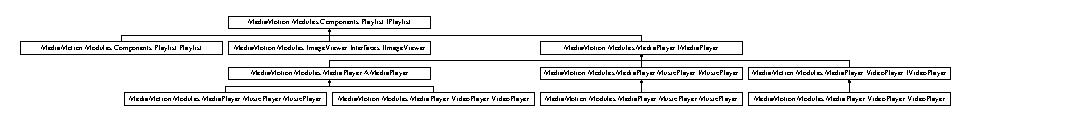
\includegraphics[height=1.197861cm]{interface_media_motion_1_1_modules_1_1_components_1_1_playlist_1_1_i_playlist}
\end{center}
\end{figure}
\subsection*{Public Member Functions}
\begin{DoxyCompactItemize}
\item 
\hypertarget{interface_media_motion_1_1_modules_1_1_components_1_1_playlist_1_1_i_playlist_a1ad0cb5984add87c6e436869985f7386}{\hyperlink{interface_media_motion_1_1_core_1_1_models_1_1_interfaces_1_1_i_element}{I\+Element} {\bfseries Current} ()}\label{interface_media_motion_1_1_modules_1_1_components_1_1_playlist_1_1_i_playlist_a1ad0cb5984add87c6e436869985f7386}

\item 
\hypertarget{interface_media_motion_1_1_modules_1_1_components_1_1_playlist_1_1_i_playlist_a34a209dfe8a4e12871cfd433ea89357f}{void {\bfseries Prev} ()}\label{interface_media_motion_1_1_modules_1_1_components_1_1_playlist_1_1_i_playlist_a34a209dfe8a4e12871cfd433ea89357f}

\item 
\hypertarget{interface_media_motion_1_1_modules_1_1_components_1_1_playlist_1_1_i_playlist_a017f72e0182525cb6b6a8dc0b7d18a21}{void {\bfseries Next} ()}\label{interface_media_motion_1_1_modules_1_1_components_1_1_playlist_1_1_i_playlist_a017f72e0182525cb6b6a8dc0b7d18a21}

\item 
\hypertarget{interface_media_motion_1_1_modules_1_1_components_1_1_playlist_1_1_i_playlist_a78275fbc8f716cdd4a547c99420bb89d}{void {\bfseries Add} (List$<$ \hyperlink{interface_media_motion_1_1_core_1_1_models_1_1_interfaces_1_1_i_element}{I\+Element} $>$ Elements)}\label{interface_media_motion_1_1_modules_1_1_components_1_1_playlist_1_1_i_playlist_a78275fbc8f716cdd4a547c99420bb89d}

\item 
\hypertarget{interface_media_motion_1_1_modules_1_1_components_1_1_playlist_1_1_i_playlist_a3e1df9682ed9c1aaa317b002224bd4dd}{void {\bfseries Remove} (List$<$ \hyperlink{interface_media_motion_1_1_core_1_1_models_1_1_interfaces_1_1_i_element}{I\+Element} $>$ Elements)}\label{interface_media_motion_1_1_modules_1_1_components_1_1_playlist_1_1_i_playlist_a3e1df9682ed9c1aaa317b002224bd4dd}

\end{DoxyCompactItemize}
\subsection*{Properties}
\begin{DoxyCompactItemize}
\item 
\hypertarget{interface_media_motion_1_1_modules_1_1_components_1_1_playlist_1_1_i_playlist_ad33154fb3b673835f80f5021813c15cb}{bool {\bfseries Random}\hspace{0.3cm}{\ttfamily  \mbox{[}get, set\mbox{]}}}\label{interface_media_motion_1_1_modules_1_1_components_1_1_playlist_1_1_i_playlist_ad33154fb3b673835f80f5021813c15cb}

\item 
\hypertarget{interface_media_motion_1_1_modules_1_1_components_1_1_playlist_1_1_i_playlist_a88003650ca0f4779df2fe2b409be7e09}{bool {\bfseries Loop}\hspace{0.3cm}{\ttfamily  \mbox{[}get, set\mbox{]}}}\label{interface_media_motion_1_1_modules_1_1_components_1_1_playlist_1_1_i_playlist_a88003650ca0f4779df2fe2b409be7e09}

\end{DoxyCompactItemize}


The documentation for this interface was generated from the following file\+:\begin{DoxyCompactItemize}
\item 
O\+:/\+Projects/\+Media\+Motion/\+Media\+Motion/\+Assets/\+Scripts/\+Modules/\+Components/\+Playlist/\+Interfaces/I\+Playlist.\+cs\end{DoxyCompactItemize}

\hypertarget{interface_media_motion_1_1_modules_1_1_components_1_1_rotate_1_1_i_rotate}{\section{Media\+Motion.\+Modules.\+Components.\+Rotate.\+I\+Rotate Interface Reference}
\label{interface_media_motion_1_1_modules_1_1_components_1_1_rotate_1_1_i_rotate}\index{Media\+Motion.\+Modules.\+Components.\+Rotate.\+I\+Rotate@{Media\+Motion.\+Modules.\+Components.\+Rotate.\+I\+Rotate}}
}
Inheritance diagram for Media\+Motion.\+Modules.\+Components.\+Rotate.\+I\+Rotate\+:\begin{figure}[H]
\begin{center}
\leavevmode
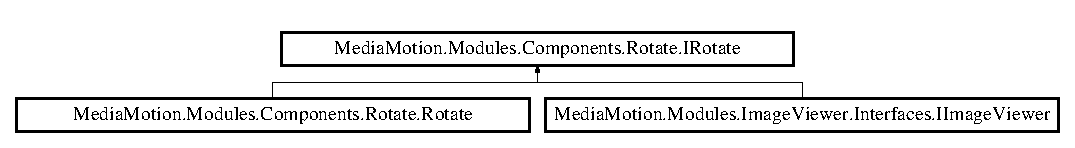
\includegraphics[height=1.546961cm]{interface_media_motion_1_1_modules_1_1_components_1_1_rotate_1_1_i_rotate}
\end{center}
\end{figure}
\subsection*{Public Member Functions}
\begin{DoxyCompactItemize}
\item 
\hypertarget{interface_media_motion_1_1_modules_1_1_components_1_1_rotate_1_1_i_rotate_a5cf1c05091e9f5061547a9017fb0385c}{void {\bfseries Rotate\+Left} ()}\label{interface_media_motion_1_1_modules_1_1_components_1_1_rotate_1_1_i_rotate_a5cf1c05091e9f5061547a9017fb0385c}

\item 
\hypertarget{interface_media_motion_1_1_modules_1_1_components_1_1_rotate_1_1_i_rotate_ac56fa99186a829f8da0d3b054e14e92a}{void {\bfseries Rotate\+Right} ()}\label{interface_media_motion_1_1_modules_1_1_components_1_1_rotate_1_1_i_rotate_ac56fa99186a829f8da0d3b054e14e92a}

\end{DoxyCompactItemize}
\subsection*{Properties}
\begin{DoxyCompactItemize}
\item 
\hypertarget{interface_media_motion_1_1_modules_1_1_components_1_1_rotate_1_1_i_rotate_ae526023d04ef483aa7b11717e50de0b4}{int {\bfseries Angle}\hspace{0.3cm}{\ttfamily  \mbox{[}get\mbox{]}}}\label{interface_media_motion_1_1_modules_1_1_components_1_1_rotate_1_1_i_rotate_ae526023d04ef483aa7b11717e50de0b4}

\end{DoxyCompactItemize}


The documentation for this interface was generated from the following file\+:\begin{DoxyCompactItemize}
\item 
O\+:/\+Projects/\+Media\+Motion/\+Media\+Motion/\+Assets/\+Scripts/\+Modules/\+Components/\+Rotate/\+Interfaces/I\+Rotate.\+cs\end{DoxyCompactItemize}

\hypertarget{interface_i_text_reader_u_i}{\section{I\+Text\+Reader\+U\+I Interface Reference}
\label{interface_i_text_reader_u_i}\index{I\+Text\+Reader\+U\+I@{I\+Text\+Reader\+U\+I}}
}
Inheritance diagram for I\+Text\+Reader\+U\+I\+:\begin{figure}[H]
\begin{center}
\leavevmode
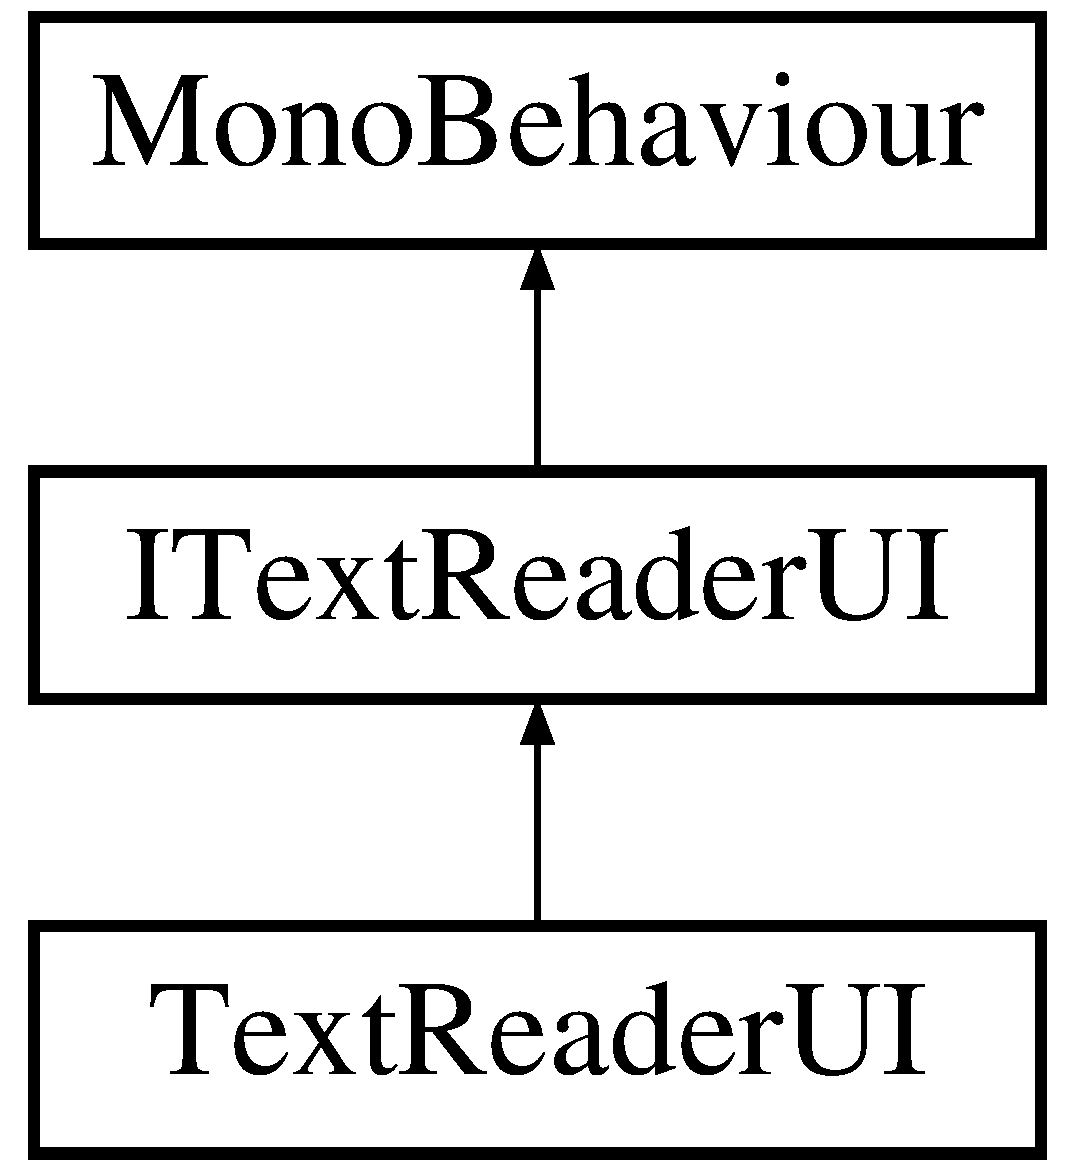
\includegraphics[height=3.000000cm]{interface_i_text_reader_u_i}
\end{center}
\end{figure}
\subsection*{Public Member Functions}
\begin{DoxyCompactItemize}
\item 
\hypertarget{interface_i_text_reader_u_i_a20c28d7da72fbca6e767bc1c67ef10c9}{void {\bfseries Start} ()}\label{interface_i_text_reader_u_i_a20c28d7da72fbca6e767bc1c67ef10c9}

\item 
\hypertarget{interface_i_text_reader_u_i_a1145f947f32e7ec05bac43c4cfd55b4f}{void {\bfseries Update} ()}\label{interface_i_text_reader_u_i_a1145f947f32e7ec05bac43c4cfd55b4f}

\end{DoxyCompactItemize}


The documentation for this interface was generated from the following file\+:\begin{DoxyCompactItemize}
\item 
O\+:/\+Projects/\+Media\+Motion/\+Media\+Motion/\+Assets/\+Scripts/\+Core/\+View/\+Interfaces/I\+Text\+Reader\+U\+I.\+cs\end{DoxyCompactItemize}

\hypertarget{interface_media_motion_1_1_modules_1_1_media_player_1_1_video_player_1_1_i_video_player}{\section{Media\+Motion.\+Modules.\+Media\+Player.\+Video\+Player.\+I\+Video\+Player Interface Reference}
\label{interface_media_motion_1_1_modules_1_1_media_player_1_1_video_player_1_1_i_video_player}\index{Media\+Motion.\+Modules.\+Media\+Player.\+Video\+Player.\+I\+Video\+Player@{Media\+Motion.\+Modules.\+Media\+Player.\+Video\+Player.\+I\+Video\+Player}}
}
Inheritance diagram for Media\+Motion.\+Modules.\+Media\+Player.\+Video\+Player.\+I\+Video\+Player\+:\begin{figure}[H]
\begin{center}
\leavevmode
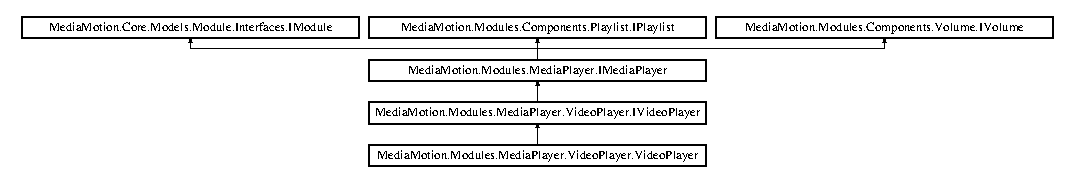
\includegraphics[height=2.007169cm]{interface_media_motion_1_1_modules_1_1_media_player_1_1_video_player_1_1_i_video_player}
\end{center}
\end{figure}
\subsection*{Additional Inherited Members}


The documentation for this interface was generated from the following file\+:\begin{DoxyCompactItemize}
\item 
O\+:/\+Projects/\+Media\+Motion/\+Media\+Motion/\+Assets/\+Scripts/\+Modules/\+Media\+Player/\+Video\+Player/I\+Video\+Player.\+cs\end{DoxyCompactItemize}

\hypertarget{interface_media_motion_1_1_modules_1_1_components_1_1_volume_1_1_i_volume}{\section{Media\+Motion.\+Modules.\+Components.\+Volume.\+I\+Volume Interface Reference}
\label{interface_media_motion_1_1_modules_1_1_components_1_1_volume_1_1_i_volume}\index{Media\+Motion.\+Modules.\+Components.\+Volume.\+I\+Volume@{Media\+Motion.\+Modules.\+Components.\+Volume.\+I\+Volume}}
}
Inheritance diagram for Media\+Motion.\+Modules.\+Components.\+Volume.\+I\+Volume\+:\begin{figure}[H]
\begin{center}
\leavevmode
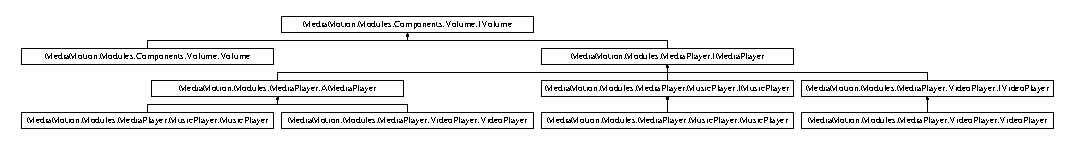
\includegraphics[height=1.497326cm]{interface_media_motion_1_1_modules_1_1_components_1_1_volume_1_1_i_volume}
\end{center}
\end{figure}
\subsection*{Public Member Functions}
\begin{DoxyCompactItemize}
\item 
\hypertarget{interface_media_motion_1_1_modules_1_1_components_1_1_volume_1_1_i_volume_a27222259ab3085631f8723952059623a}{void {\bfseries Volume\+Up} ()}\label{interface_media_motion_1_1_modules_1_1_components_1_1_volume_1_1_i_volume_a27222259ab3085631f8723952059623a}

\item 
\hypertarget{interface_media_motion_1_1_modules_1_1_components_1_1_volume_1_1_i_volume_a079aa9e43fd201125391e17c86f83e6c}{void {\bfseries Volume\+Down} ()}\label{interface_media_motion_1_1_modules_1_1_components_1_1_volume_1_1_i_volume_a079aa9e43fd201125391e17c86f83e6c}

\end{DoxyCompactItemize}
\subsection*{Properties}
\begin{DoxyCompactItemize}
\item 
\hypertarget{interface_media_motion_1_1_modules_1_1_components_1_1_volume_1_1_i_volume_af7b1970ffa7e18357bf3af3597e9e014}{int {\bfseries Sound}\hspace{0.3cm}{\ttfamily  \mbox{[}get\mbox{]}}}\label{interface_media_motion_1_1_modules_1_1_components_1_1_volume_1_1_i_volume_af7b1970ffa7e18357bf3af3597e9e014}

\item 
\hypertarget{interface_media_motion_1_1_modules_1_1_components_1_1_volume_1_1_i_volume_aec2c2cfe378cc0e99477d26a1e346f96}{int {\bfseries Step}\hspace{0.3cm}{\ttfamily  \mbox{[}get\mbox{]}}}\label{interface_media_motion_1_1_modules_1_1_components_1_1_volume_1_1_i_volume_aec2c2cfe378cc0e99477d26a1e346f96}

\end{DoxyCompactItemize}


The documentation for this interface was generated from the following file\+:\begin{DoxyCompactItemize}
\item 
O\+:/\+Projects/\+Media\+Motion/\+Media\+Motion/\+Assets/\+Scripts/\+Modules/\+Components/\+Volume/\+Interfaces/I\+Volume.\+cs\end{DoxyCompactItemize}

\hypertarget{interface_i_wheel_tool_u_i}{\section{I\+Wheel\+Tool\+U\+I Interface Reference}
\label{interface_i_wheel_tool_u_i}\index{I\+Wheel\+Tool\+U\+I@{I\+Wheel\+Tool\+U\+I}}
}
Inheritance diagram for I\+Wheel\+Tool\+U\+I\+:\begin{figure}[H]
\begin{center}
\leavevmode
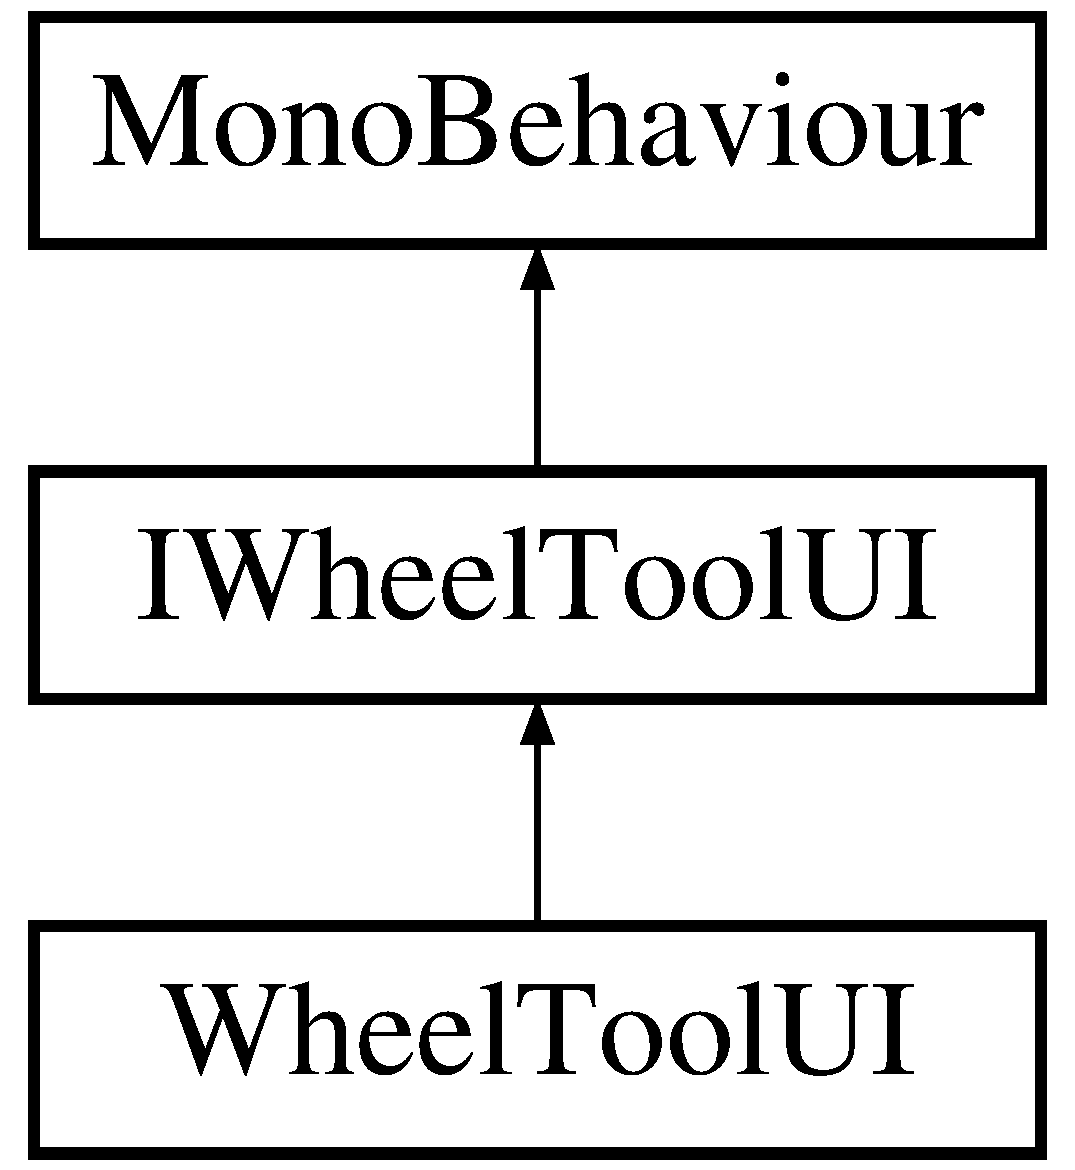
\includegraphics[height=3.000000cm]{interface_i_wheel_tool_u_i}
\end{center}
\end{figure}
\subsection*{Public Member Functions}
\begin{DoxyCompactItemize}
\item 
\hypertarget{interface_i_wheel_tool_u_i_a79906de3461b6e8001b5a6524865269c}{void {\bfseries Start} ()}\label{interface_i_wheel_tool_u_i_a79906de3461b6e8001b5a6524865269c}

\item 
\hypertarget{interface_i_wheel_tool_u_i_a9275a64052867ecc6b64f30f04dbccfe}{void {\bfseries Update} ()}\label{interface_i_wheel_tool_u_i_a9275a64052867ecc6b64f30f04dbccfe}

\end{DoxyCompactItemize}


The documentation for this interface was generated from the following file\+:\begin{DoxyCompactItemize}
\item 
O\+:/\+Projects/\+Media\+Motion/\+Media\+Motion/\+Assets/\+Scripts/\+Core/\+View/\+Interfaces/I\+Wheel\+Tool\+U\+I.\+cs\end{DoxyCompactItemize}

\hypertarget{interface_media_motion_1_1_core_1_1_models_1_1_wrapper_1_1_interfaces_1_1_i_wrapper}{\section{Media\+Motion.\+Core.\+Models.\+Wrapper.\+Interfaces.\+I\+Wrapper Interface Reference}
\label{interface_media_motion_1_1_core_1_1_models_1_1_wrapper_1_1_interfaces_1_1_i_wrapper}\index{Media\+Motion.\+Core.\+Models.\+Wrapper.\+Interfaces.\+I\+Wrapper@{Media\+Motion.\+Core.\+Models.\+Wrapper.\+Interfaces.\+I\+Wrapper}}
}


The documentation for this interface was generated from the following file\+:\begin{DoxyCompactItemize}
\item 
O\+:/\+Projects/\+Media\+Motion/\+Media\+Motion/\+Assets/\+Scripts/\+Core/\+Models/\+Wrapper/\+Interfaces/I\+Wrapper.\+cs\end{DoxyCompactItemize}

\hypertarget{interface_media_motion_1_1_modules_1_1_components_1_1_zoom_1_1_i_zoom}{\section{Media\+Motion.\+Modules.\+Components.\+Zoom.\+I\+Zoom Interface Reference}
\label{interface_media_motion_1_1_modules_1_1_components_1_1_zoom_1_1_i_zoom}\index{Media\+Motion.\+Modules.\+Components.\+Zoom.\+I\+Zoom@{Media\+Motion.\+Modules.\+Components.\+Zoom.\+I\+Zoom}}
}
Inheritance diagram for Media\+Motion.\+Modules.\+Components.\+Zoom.\+I\+Zoom\+:\begin{figure}[H]
\begin{center}
\leavevmode
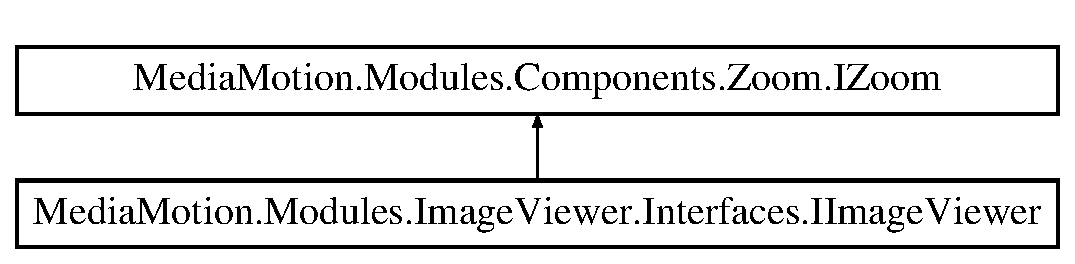
\includegraphics[height=2.000000cm]{interface_media_motion_1_1_modules_1_1_components_1_1_zoom_1_1_i_zoom}
\end{center}
\end{figure}
\subsection*{Public Member Functions}
\begin{DoxyCompactItemize}
\item 
\hypertarget{interface_media_motion_1_1_modules_1_1_components_1_1_zoom_1_1_i_zoom_ab437e7aac62f2b6a468ccae121405c49}{void {\bfseries Zoom\+In} ()}\label{interface_media_motion_1_1_modules_1_1_components_1_1_zoom_1_1_i_zoom_ab437e7aac62f2b6a468ccae121405c49}

\item 
\hypertarget{interface_media_motion_1_1_modules_1_1_components_1_1_zoom_1_1_i_zoom_a9da4f57dd95348976bf1ad2d3fceaffd}{void {\bfseries Zoom\+Out} ()}\label{interface_media_motion_1_1_modules_1_1_components_1_1_zoom_1_1_i_zoom_a9da4f57dd95348976bf1ad2d3fceaffd}

\end{DoxyCompactItemize}
\subsection*{Properties}
\begin{DoxyCompactItemize}
\item 
\hypertarget{interface_media_motion_1_1_modules_1_1_components_1_1_zoom_1_1_i_zoom_af3224ae49009155024873364ddfee40a}{float {\bfseries Coeff}\hspace{0.3cm}{\ttfamily  \mbox{[}get\mbox{]}}}\label{interface_media_motion_1_1_modules_1_1_components_1_1_zoom_1_1_i_zoom_af3224ae49009155024873364ddfee40a}

\end{DoxyCompactItemize}


The documentation for this interface was generated from the following file\+:\begin{DoxyCompactItemize}
\item 
O\+:/\+Projects/\+Media\+Motion/\+Media\+Motion/\+Assets/\+Scripts/\+Modules/\+Components/\+Zoom/\+Interfaces/I\+Zoom.\+cs\end{DoxyCompactItemize}

\hypertarget{class_media_motion_1_1_modules_1_1_media_player_1_1_events_1_1_media_event_args}{\section{Media\+Motion.\+Modules.\+Media\+Player.\+Events.\+Media\+Event\+Args Class Reference}
\label{class_media_motion_1_1_modules_1_1_media_player_1_1_events_1_1_media_event_args}\index{Media\+Motion.\+Modules.\+Media\+Player.\+Events.\+Media\+Event\+Args@{Media\+Motion.\+Modules.\+Media\+Player.\+Events.\+Media\+Event\+Args}}
}
Inheritance diagram for Media\+Motion.\+Modules.\+Media\+Player.\+Events.\+Media\+Event\+Args\+:\begin{figure}[H]
\begin{center}
\leavevmode
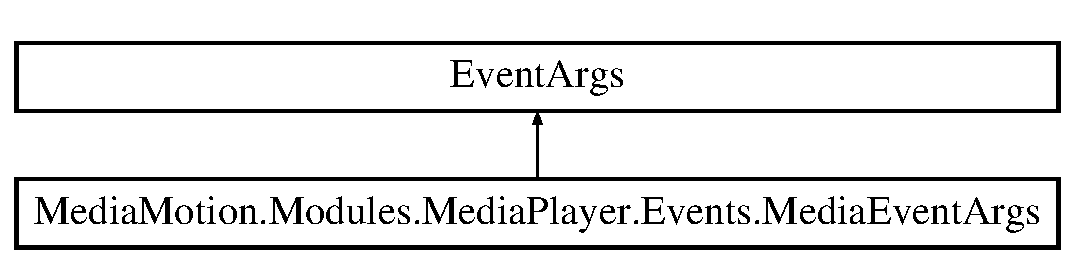
\includegraphics[height=2.000000cm]{class_media_motion_1_1_modules_1_1_media_player_1_1_events_1_1_media_event_args}
\end{center}
\end{figure}
\subsection*{Public Member Functions}
\begin{DoxyCompactItemize}
\item 
\hypertarget{class_media_motion_1_1_modules_1_1_media_player_1_1_events_1_1_media_event_args_a4052483bf9145836864f5f3c1ae08ecd}{{\bfseries Media\+Event\+Args} (\hyperlink{interface_media_motion_1_1_core_1_1_models_1_1_interfaces_1_1_i_element}{I\+Element} Element)}\label{class_media_motion_1_1_modules_1_1_media_player_1_1_events_1_1_media_event_args_a4052483bf9145836864f5f3c1ae08ecd}

\end{DoxyCompactItemize}
\subsection*{Properties}
\begin{DoxyCompactItemize}
\item 
\hypertarget{class_media_motion_1_1_modules_1_1_media_player_1_1_events_1_1_media_event_args_ac18a4b5750d0414eba87893d867649e2}{\hyperlink{interface_media_motion_1_1_core_1_1_models_1_1_interfaces_1_1_i_element}{I\+Element} {\bfseries Element}\hspace{0.3cm}{\ttfamily  \mbox{[}get\mbox{]}}}\label{class_media_motion_1_1_modules_1_1_media_player_1_1_events_1_1_media_event_args_ac18a4b5750d0414eba87893d867649e2}

\end{DoxyCompactItemize}


The documentation for this class was generated from the following file\+:\begin{DoxyCompactItemize}
\item 
O\+:/\+Projects/\+Media\+Motion/\+Media\+Motion/\+Assets/\+Scripts/\+Modules/\+Media\+Player/\+Events/Media\+Event\+Args.\+cs\end{DoxyCompactItemize}

\hypertarget{class_media_motion_1_1_core_1_1_controllers_1_1_media_motion_controller}{\section{Media\+Motion.\+Core.\+Controllers.\+Media\+Motion\+Controller Class Reference}
\label{class_media_motion_1_1_core_1_1_controllers_1_1_media_motion_controller}\index{Media\+Motion.\+Core.\+Controllers.\+Media\+Motion\+Controller@{Media\+Motion.\+Core.\+Controllers.\+Media\+Motion\+Controller}}
}
Inheritance diagram for Media\+Motion.\+Core.\+Controllers.\+Media\+Motion\+Controller\+:\begin{figure}[H]
\begin{center}
\leavevmode
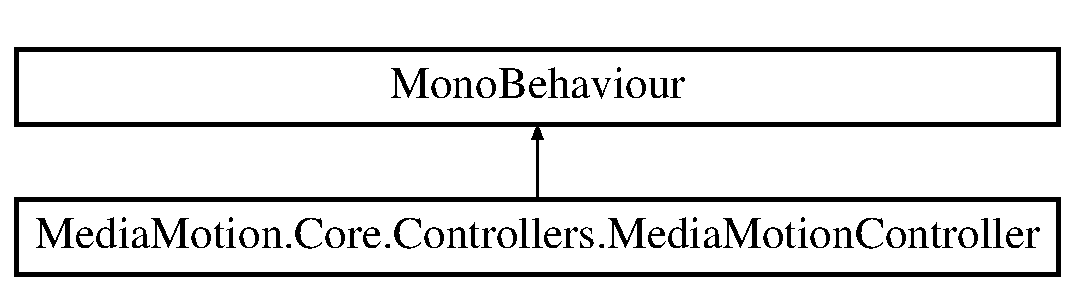
\includegraphics[height=2.000000cm]{class_media_motion_1_1_core_1_1_controllers_1_1_media_motion_controller}
\end{center}
\end{figure}


The documentation for this class was generated from the following file\+:\begin{DoxyCompactItemize}
\item 
O\+:/\+Projects/\+Media\+Motion/\+Media\+Motion/\+Assets/\+Scripts/\+Core/\+Controllers/Media\+Motion\+Controller.\+cs\end{DoxyCompactItemize}

\hypertarget{class_media_player_u_i}{\section{Media\+Player\+U\+I Class Reference}
\label{class_media_player_u_i}\index{Media\+Player\+U\+I@{Media\+Player\+U\+I}}
}
Inheritance diagram for Media\+Player\+U\+I\+:\begin{figure}[H]
\begin{center}
\leavevmode
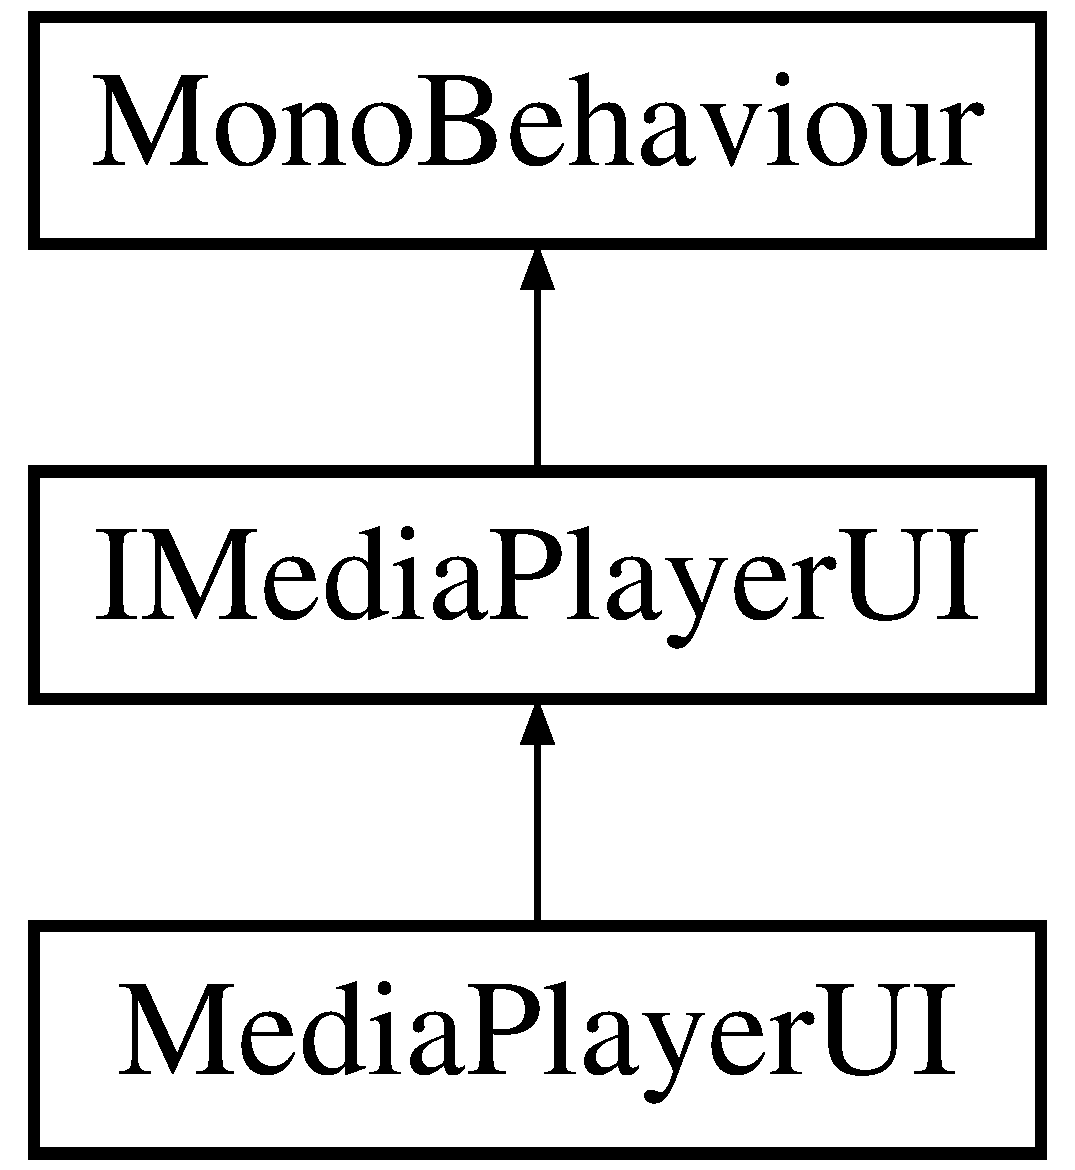
\includegraphics[height=3.000000cm]{class_media_player_u_i}
\end{center}
\end{figure}
\subsection*{Additional Inherited Members}


The documentation for this class was generated from the following file\+:\begin{DoxyCompactItemize}
\item 
O\+:/\+Projects/\+Media\+Motion/\+Media\+Motion/\+Assets/\+Scripts/\+Core/\+View/Media\+Player\+U\+I.\+cs\end{DoxyCompactItemize}

\hypertarget{class_media_motion_1_1_modules_1_1_media_player_1_1_music_player_1_1_music_player}{\section{Media\+Motion.\+Modules.\+Media\+Player.\+Music\+Player.\+Music\+Player Class Reference}
\label{class_media_motion_1_1_modules_1_1_media_player_1_1_music_player_1_1_music_player}\index{Media\+Motion.\+Modules.\+Media\+Player.\+Music\+Player.\+Music\+Player@{Media\+Motion.\+Modules.\+Media\+Player.\+Music\+Player.\+Music\+Player}}
}
Inheritance diagram for Media\+Motion.\+Modules.\+Media\+Player.\+Music\+Player.\+Music\+Player\+:\begin{figure}[H]
\begin{center}
\leavevmode
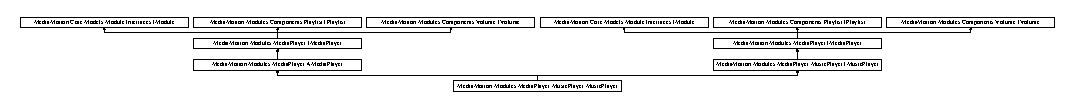
\includegraphics[height=0.998218cm]{class_media_motion_1_1_modules_1_1_media_player_1_1_music_player_1_1_music_player}
\end{center}
\end{figure}
\subsection*{Public Member Functions}
\begin{DoxyCompactItemize}
\item 
\hypertarget{class_media_motion_1_1_modules_1_1_media_player_1_1_music_player_1_1_music_player_ad3c6d8dca403d823575e1ad6135657ff}{override void {\bfseries Play} ()}\label{class_media_motion_1_1_modules_1_1_media_player_1_1_music_player_1_1_music_player_ad3c6d8dca403d823575e1ad6135657ff}

\item 
\hypertarget{class_media_motion_1_1_modules_1_1_media_player_1_1_music_player_1_1_music_player_ab4ac12829d097ea3972af1eebe67e571}{override void {\bfseries Pause} ()}\label{class_media_motion_1_1_modules_1_1_media_player_1_1_music_player_1_1_music_player_ab4ac12829d097ea3972af1eebe67e571}

\item 
\hypertarget{class_media_motion_1_1_modules_1_1_media_player_1_1_music_player_1_1_music_player_adb718d8b3ec481202486595f7d1f661c}{override void {\bfseries Stop} ()}\label{class_media_motion_1_1_modules_1_1_media_player_1_1_music_player_1_1_music_player_adb718d8b3ec481202486595f7d1f661c}

\end{DoxyCompactItemize}
\subsection*{Additional Inherited Members}


The documentation for this class was generated from the following file\+:\begin{DoxyCompactItemize}
\item 
O\+:/\+Projects/\+Media\+Motion/\+Media\+Motion/\+Assets/\+Scripts/\+Modules/\+Media\+Player/\+Music\+Player/Music\+Player.\+cs\end{DoxyCompactItemize}

\hypertarget{class_media_motion_1_1_core_1_1_models_1_1_p_d_f}{\section{Media\+Motion.\+Core.\+Models.\+P\+D\+F Class Reference}
\label{class_media_motion_1_1_core_1_1_models_1_1_p_d_f}\index{Media\+Motion.\+Core.\+Models.\+P\+D\+F@{Media\+Motion.\+Core.\+Models.\+P\+D\+F}}
}
Inheritance diagram for Media\+Motion.\+Core.\+Models.\+P\+D\+F\+:\begin{figure}[H]
\begin{center}
\leavevmode
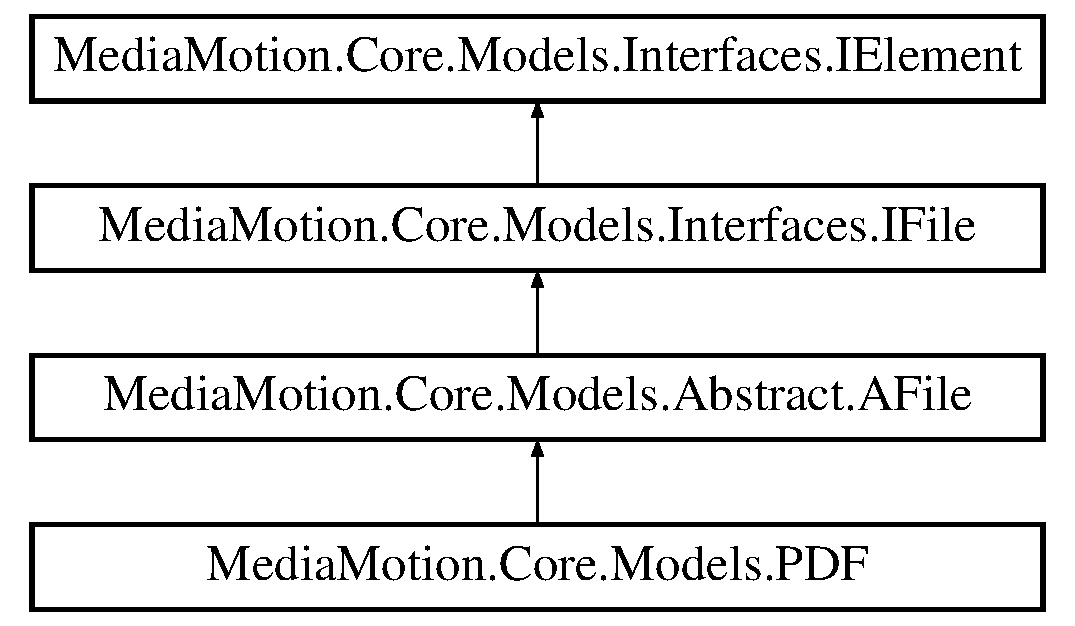
\includegraphics[height=4.000000cm]{class_media_motion_1_1_core_1_1_models_1_1_p_d_f}
\end{center}
\end{figure}
\subsection*{Additional Inherited Members}


The documentation for this class was generated from the following file\+:\begin{DoxyCompactItemize}
\item 
O\+:/\+Projects/\+Media\+Motion/\+Media\+Motion/\+Assets/\+Scripts/\+Core/\+Models/\+File\+Manager/P\+D\+F.\+cs\end{DoxyCompactItemize}

\hypertarget{class_media_motion_1_1_modules_1_1_components_1_1_playlist_1_1_playlist}{\section{Media\+Motion.\+Modules.\+Components.\+Playlist.\+Playlist Class Reference}
\label{class_media_motion_1_1_modules_1_1_components_1_1_playlist_1_1_playlist}\index{Media\+Motion.\+Modules.\+Components.\+Playlist.\+Playlist@{Media\+Motion.\+Modules.\+Components.\+Playlist.\+Playlist}}
}
Inheritance diagram for Media\+Motion.\+Modules.\+Components.\+Playlist.\+Playlist\+:\begin{figure}[H]
\begin{center}
\leavevmode
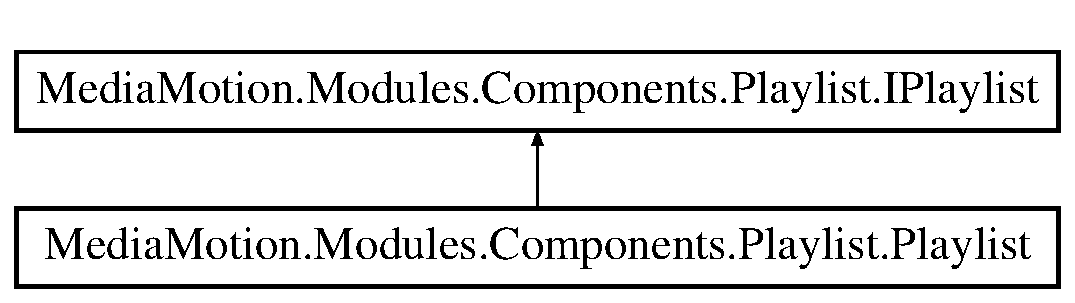
\includegraphics[height=2.000000cm]{class_media_motion_1_1_modules_1_1_components_1_1_playlist_1_1_playlist}
\end{center}
\end{figure}
\subsection*{Public Member Functions}
\begin{DoxyCompactItemize}
\item 
\hypertarget{class_media_motion_1_1_modules_1_1_components_1_1_playlist_1_1_playlist_afe2c90bf65e6c602134d6855eb719046}{delegate void {\bfseries Playlist\+Element\+Change\+Handler} (object sender, \hyperlink{class_media_motion_1_1_modules_1_1_components_1_1_playlist_1_1_events_1_1_playlist_element_change_event_args}{Playlist\+Element\+Change\+Event\+Args} e)}\label{class_media_motion_1_1_modules_1_1_components_1_1_playlist_1_1_playlist_afe2c90bf65e6c602134d6855eb719046}

\item 
\hypertarget{class_media_motion_1_1_modules_1_1_components_1_1_playlist_1_1_playlist_a4d6d093a372a5e0909aecbf339d013f6}{delegate void {\bfseries Playlist\+Change\+Handler} (object sender, \hyperlink{class_media_motion_1_1_modules_1_1_components_1_1_playlist_1_1_events_1_1_playlist_change_event_args}{Playlist\+Change\+Event\+Args} e)}\label{class_media_motion_1_1_modules_1_1_components_1_1_playlist_1_1_playlist_a4d6d093a372a5e0909aecbf339d013f6}

\item 
\hypertarget{class_media_motion_1_1_modules_1_1_components_1_1_playlist_1_1_playlist_aaa0f71cc951631f2f05c287cffe9d64b}{{\bfseries Playlist} (bool Loop=true, bool Random=false)}\label{class_media_motion_1_1_modules_1_1_components_1_1_playlist_1_1_playlist_aaa0f71cc951631f2f05c287cffe9d64b}

\item 
\hypertarget{class_media_motion_1_1_modules_1_1_components_1_1_playlist_1_1_playlist_ad180bca0034027f3776f71dc3acaa3a2}{\hyperlink{interface_media_motion_1_1_core_1_1_models_1_1_interfaces_1_1_i_element}{I\+Element} {\bfseries Current} ()}\label{class_media_motion_1_1_modules_1_1_components_1_1_playlist_1_1_playlist_ad180bca0034027f3776f71dc3acaa3a2}

\item 
\hypertarget{class_media_motion_1_1_modules_1_1_components_1_1_playlist_1_1_playlist_a27629b345ac08920422898c79aca3d79}{void {\bfseries Prev} ()}\label{class_media_motion_1_1_modules_1_1_components_1_1_playlist_1_1_playlist_a27629b345ac08920422898c79aca3d79}

\item 
\hypertarget{class_media_motion_1_1_modules_1_1_components_1_1_playlist_1_1_playlist_a7f684e4fc067e47b7041127c7f8ea5fc}{void {\bfseries Next} ()}\label{class_media_motion_1_1_modules_1_1_components_1_1_playlist_1_1_playlist_a7f684e4fc067e47b7041127c7f8ea5fc}

\item 
\hypertarget{class_media_motion_1_1_modules_1_1_components_1_1_playlist_1_1_playlist_a3c61725444e5553d60d788dfabdcac8c}{void {\bfseries Add} (List$<$ \hyperlink{interface_media_motion_1_1_core_1_1_models_1_1_interfaces_1_1_i_element}{I\+Element} $>$ Elements)}\label{class_media_motion_1_1_modules_1_1_components_1_1_playlist_1_1_playlist_a3c61725444e5553d60d788dfabdcac8c}

\item 
\hypertarget{class_media_motion_1_1_modules_1_1_components_1_1_playlist_1_1_playlist_af7bd8105e1063e49bd9ef7afde1fe329}{void {\bfseries Remove} (List$<$ \hyperlink{interface_media_motion_1_1_core_1_1_models_1_1_interfaces_1_1_i_element}{I\+Element} $>$ Elements)}\label{class_media_motion_1_1_modules_1_1_components_1_1_playlist_1_1_playlist_af7bd8105e1063e49bd9ef7afde1fe329}

\end{DoxyCompactItemize}
\subsection*{Properties}
\begin{DoxyCompactItemize}
\item 
\hypertarget{class_media_motion_1_1_modules_1_1_components_1_1_playlist_1_1_playlist_ac293f0b3e77b15d3eb60747f75c29ba4}{bool {\bfseries Random}\hspace{0.3cm}{\ttfamily  \mbox{[}get, set\mbox{]}}}\label{class_media_motion_1_1_modules_1_1_components_1_1_playlist_1_1_playlist_ac293f0b3e77b15d3eb60747f75c29ba4}

\item 
\hypertarget{class_media_motion_1_1_modules_1_1_components_1_1_playlist_1_1_playlist_a393cb97cede7dc4b3b624b9e51c2a32a}{bool {\bfseries Loop}\hspace{0.3cm}{\ttfamily  \mbox{[}get, set\mbox{]}}}\label{class_media_motion_1_1_modules_1_1_components_1_1_playlist_1_1_playlist_a393cb97cede7dc4b3b624b9e51c2a32a}

\end{DoxyCompactItemize}
\subsection*{Events}
\begin{DoxyCompactItemize}
\item 
\hypertarget{class_media_motion_1_1_modules_1_1_components_1_1_playlist_1_1_playlist_acd79347d70f2e77035bc1475b8928b5c}{Playlist\+Element\+Change\+Handler {\bfseries On\+Element\+Change}}\label{class_media_motion_1_1_modules_1_1_components_1_1_playlist_1_1_playlist_acd79347d70f2e77035bc1475b8928b5c}

\item 
\hypertarget{class_media_motion_1_1_modules_1_1_components_1_1_playlist_1_1_playlist_a1d84b782096b8cadd6ef68f64dec80e3}{Playlist\+Change\+Handler {\bfseries On\+Playlist\+Change}}\label{class_media_motion_1_1_modules_1_1_components_1_1_playlist_1_1_playlist_a1d84b782096b8cadd6ef68f64dec80e3}

\end{DoxyCompactItemize}


The documentation for this class was generated from the following file\+:\begin{DoxyCompactItemize}
\item 
O\+:/\+Projects/\+Media\+Motion/\+Media\+Motion/\+Assets/\+Scripts/\+Modules/\+Components/\+Playlist/Playlist.\+cs\end{DoxyCompactItemize}

\hypertarget{class_media_motion_1_1_modules_1_1_components_1_1_playlist_1_1_events_1_1_playlist_change_event_args}{\section{Media\+Motion.\+Modules.\+Components.\+Playlist.\+Events.\+Playlist\+Change\+Event\+Args Class Reference}
\label{class_media_motion_1_1_modules_1_1_components_1_1_playlist_1_1_events_1_1_playlist_change_event_args}\index{Media\+Motion.\+Modules.\+Components.\+Playlist.\+Events.\+Playlist\+Change\+Event\+Args@{Media\+Motion.\+Modules.\+Components.\+Playlist.\+Events.\+Playlist\+Change\+Event\+Args}}
}
Inheritance diagram for Media\+Motion.\+Modules.\+Components.\+Playlist.\+Events.\+Playlist\+Change\+Event\+Args\+:\begin{figure}[H]
\begin{center}
\leavevmode
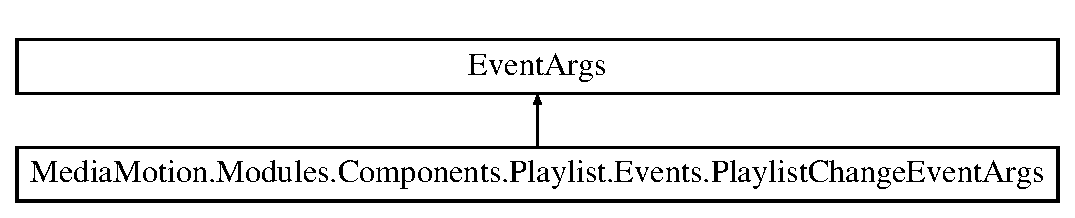
\includegraphics[height=2.000000cm]{class_media_motion_1_1_modules_1_1_components_1_1_playlist_1_1_events_1_1_playlist_change_event_args}
\end{center}
\end{figure}
\subsection*{Public Member Functions}
\begin{DoxyCompactItemize}
\item 
\hypertarget{class_media_motion_1_1_modules_1_1_components_1_1_playlist_1_1_events_1_1_playlist_change_event_args_a08d2f9853f428dd6df0a200c79b97a5d}{{\bfseries Playlist\+Change\+Event\+Args} (List$<$ \hyperlink{interface_media_motion_1_1_core_1_1_models_1_1_interfaces_1_1_i_element}{I\+Element} $>$ Elements)}\label{class_media_motion_1_1_modules_1_1_components_1_1_playlist_1_1_events_1_1_playlist_change_event_args_a08d2f9853f428dd6df0a200c79b97a5d}

\end{DoxyCompactItemize}
\subsection*{Properties}
\begin{DoxyCompactItemize}
\item 
\hypertarget{class_media_motion_1_1_modules_1_1_components_1_1_playlist_1_1_events_1_1_playlist_change_event_args_a8367ec884414f33038540efe88a8df98}{List$<$ \hyperlink{interface_media_motion_1_1_core_1_1_models_1_1_interfaces_1_1_i_element}{I\+Element} $>$ {\bfseries Elements}\hspace{0.3cm}{\ttfamily  \mbox{[}get\mbox{]}}}\label{class_media_motion_1_1_modules_1_1_components_1_1_playlist_1_1_events_1_1_playlist_change_event_args_a8367ec884414f33038540efe88a8df98}

\end{DoxyCompactItemize}


The documentation for this class was generated from the following file\+:\begin{DoxyCompactItemize}
\item 
O\+:/\+Projects/\+Media\+Motion/\+Media\+Motion/\+Assets/\+Scripts/\+Modules/\+Components/\+Playlist/\+Events/Playlist\+Change\+Event\+Args.\+cs\end{DoxyCompactItemize}

\hypertarget{class_media_motion_1_1_modules_1_1_components_1_1_playlist_1_1_events_1_1_playlist_element_change_event_args}{\section{Media\+Motion.\+Modules.\+Components.\+Playlist.\+Events.\+Playlist\+Element\+Change\+Event\+Args Class Reference}
\label{class_media_motion_1_1_modules_1_1_components_1_1_playlist_1_1_events_1_1_playlist_element_change_event_args}\index{Media\+Motion.\+Modules.\+Components.\+Playlist.\+Events.\+Playlist\+Element\+Change\+Event\+Args@{Media\+Motion.\+Modules.\+Components.\+Playlist.\+Events.\+Playlist\+Element\+Change\+Event\+Args}}
}
Inheritance diagram for Media\+Motion.\+Modules.\+Components.\+Playlist.\+Events.\+Playlist\+Element\+Change\+Event\+Args\+:\begin{figure}[H]
\begin{center}
\leavevmode
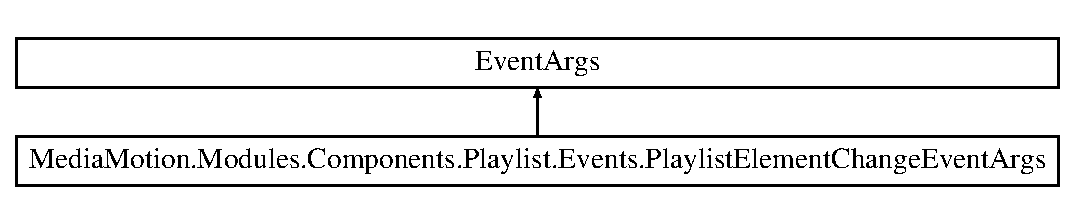
\includegraphics[height=2.000000cm]{class_media_motion_1_1_modules_1_1_components_1_1_playlist_1_1_events_1_1_playlist_element_change_event_args}
\end{center}
\end{figure}
\subsection*{Public Member Functions}
\begin{DoxyCompactItemize}
\item 
\hypertarget{class_media_motion_1_1_modules_1_1_components_1_1_playlist_1_1_events_1_1_playlist_element_change_event_args_a9f3badd8dff362075840698d866dfdf8}{{\bfseries Playlist\+Element\+Change\+Event\+Args} (\hyperlink{interface_media_motion_1_1_core_1_1_models_1_1_interfaces_1_1_i_element}{I\+Element} Previous, \hyperlink{interface_media_motion_1_1_core_1_1_models_1_1_interfaces_1_1_i_element}{I\+Element} Current)}\label{class_media_motion_1_1_modules_1_1_components_1_1_playlist_1_1_events_1_1_playlist_element_change_event_args_a9f3badd8dff362075840698d866dfdf8}

\end{DoxyCompactItemize}
\subsection*{Properties}
\begin{DoxyCompactItemize}
\item 
\hypertarget{class_media_motion_1_1_modules_1_1_components_1_1_playlist_1_1_events_1_1_playlist_element_change_event_args_a2e8e1d85d13e7c7d96deb54bdb919fdf}{\hyperlink{interface_media_motion_1_1_core_1_1_models_1_1_interfaces_1_1_i_element}{I\+Element} {\bfseries Previous}\hspace{0.3cm}{\ttfamily  \mbox{[}get\mbox{]}}}\label{class_media_motion_1_1_modules_1_1_components_1_1_playlist_1_1_events_1_1_playlist_element_change_event_args_a2e8e1d85d13e7c7d96deb54bdb919fdf}

\item 
\hypertarget{class_media_motion_1_1_modules_1_1_components_1_1_playlist_1_1_events_1_1_playlist_element_change_event_args_a11fd9c96208baf04f8ed428cddb37578}{\hyperlink{interface_media_motion_1_1_core_1_1_models_1_1_interfaces_1_1_i_element}{I\+Element} {\bfseries Current}\hspace{0.3cm}{\ttfamily  \mbox{[}get\mbox{]}}}\label{class_media_motion_1_1_modules_1_1_components_1_1_playlist_1_1_events_1_1_playlist_element_change_event_args_a11fd9c96208baf04f8ed428cddb37578}

\end{DoxyCompactItemize}


The documentation for this class was generated from the following file\+:\begin{DoxyCompactItemize}
\item 
O\+:/\+Projects/\+Media\+Motion/\+Media\+Motion/\+Assets/\+Scripts/\+Modules/\+Components/\+Playlist/\+Events/Playlist\+Element\+Change\+Event\+Args.\+cs\end{DoxyCompactItemize}

\hypertarget{class_media_motion_1_1_core_1_1_models_1_1_regular}{\section{Media\+Motion.\+Core.\+Models.\+Regular Class Reference}
\label{class_media_motion_1_1_core_1_1_models_1_1_regular}\index{Media\+Motion.\+Core.\+Models.\+Regular@{Media\+Motion.\+Core.\+Models.\+Regular}}
}
Inheritance diagram for Media\+Motion.\+Core.\+Models.\+Regular\+:\begin{figure}[H]
\begin{center}
\leavevmode
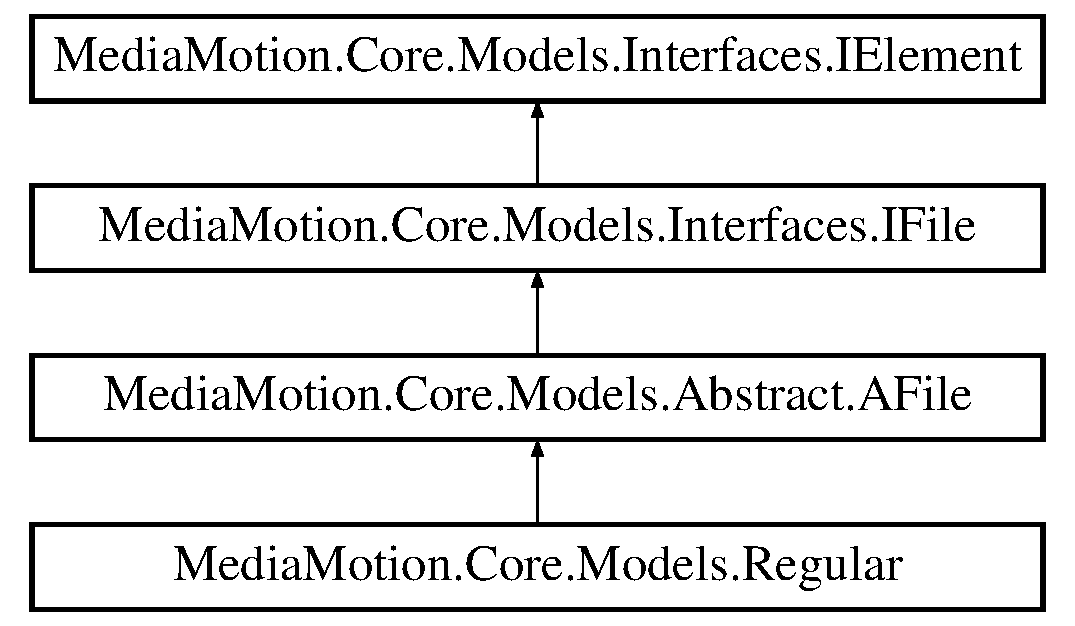
\includegraphics[height=4.000000cm]{class_media_motion_1_1_core_1_1_models_1_1_regular}
\end{center}
\end{figure}
\subsection*{Additional Inherited Members}


The documentation for this class was generated from the following file\+:\begin{DoxyCompactItemize}
\item 
O\+:/\+Projects/\+Media\+Motion/\+Media\+Motion/\+Assets/\+Scripts/\+Core/\+Models/\+File\+Manager/Regular.\+cs\end{DoxyCompactItemize}

\hypertarget{class_media_motion_1_1_modules_1_1_components_1_1_rotate_1_1_rotate}{\section{Media\+Motion.\+Modules.\+Components.\+Rotate.\+Rotate Class Reference}
\label{class_media_motion_1_1_modules_1_1_components_1_1_rotate_1_1_rotate}\index{Media\+Motion.\+Modules.\+Components.\+Rotate.\+Rotate@{Media\+Motion.\+Modules.\+Components.\+Rotate.\+Rotate}}
}
Inheritance diagram for Media\+Motion.\+Modules.\+Components.\+Rotate.\+Rotate\+:\begin{figure}[H]
\begin{center}
\leavevmode
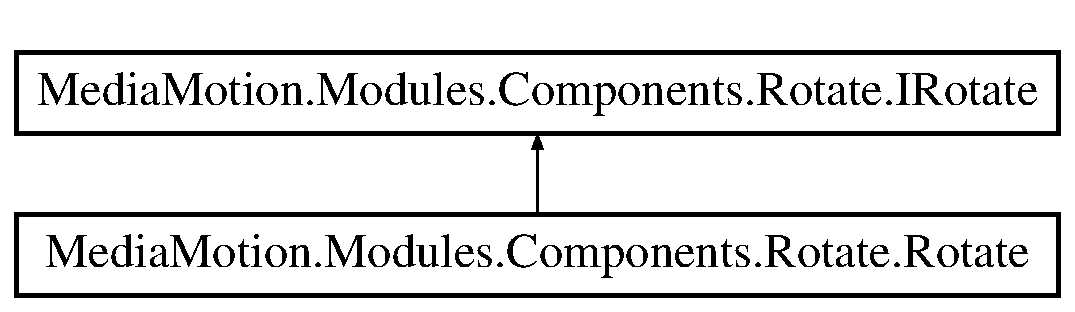
\includegraphics[height=2.000000cm]{class_media_motion_1_1_modules_1_1_components_1_1_rotate_1_1_rotate}
\end{center}
\end{figure}
\subsection*{Public Member Functions}
\begin{DoxyCompactItemize}
\item 
\hypertarget{class_media_motion_1_1_modules_1_1_components_1_1_rotate_1_1_rotate_ad73946e8cf6ebecf8aae436da614658e}{delegate void {\bfseries Rotate\+Handler} (object sender, \hyperlink{class_media_motion_1_1_modules_1_1_components_1_1_rotate_1_1_events_1_1_rotate_event_args}{Rotate\+Event\+Args} e)}\label{class_media_motion_1_1_modules_1_1_components_1_1_rotate_1_1_rotate_ad73946e8cf6ebecf8aae436da614658e}

\item 
\hypertarget{class_media_motion_1_1_modules_1_1_components_1_1_rotate_1_1_rotate_a58f3aa9778c0fdc2ae3f9de2d92b3e66}{void {\bfseries Rotate\+Left} ()}\label{class_media_motion_1_1_modules_1_1_components_1_1_rotate_1_1_rotate_a58f3aa9778c0fdc2ae3f9de2d92b3e66}

\item 
\hypertarget{class_media_motion_1_1_modules_1_1_components_1_1_rotate_1_1_rotate_a3b740126dcc04d7cacb3b0a7089d9bc4}{void {\bfseries Rotate\+Right} ()}\label{class_media_motion_1_1_modules_1_1_components_1_1_rotate_1_1_rotate_a3b740126dcc04d7cacb3b0a7089d9bc4}

\end{DoxyCompactItemize}
\subsection*{Protected Member Functions}
\begin{DoxyCompactItemize}
\item 
\hypertarget{class_media_motion_1_1_modules_1_1_components_1_1_rotate_1_1_rotate_a25abdd66879453b43741255769b3e5fc}{void {\bfseries Normalize} ()}\label{class_media_motion_1_1_modules_1_1_components_1_1_rotate_1_1_rotate_a25abdd66879453b43741255769b3e5fc}

\end{DoxyCompactItemize}
\subsection*{Properties}
\begin{DoxyCompactItemize}
\item 
\hypertarget{class_media_motion_1_1_modules_1_1_components_1_1_rotate_1_1_rotate_ab0c9c818f58e1c91f32fad2f1cd61713}{int {\bfseries Angle}\hspace{0.3cm}{\ttfamily  \mbox{[}get\mbox{]}}}\label{class_media_motion_1_1_modules_1_1_components_1_1_rotate_1_1_rotate_ab0c9c818f58e1c91f32fad2f1cd61713}

\end{DoxyCompactItemize}
\subsection*{Events}
\begin{DoxyCompactItemize}
\item 
\hypertarget{class_media_motion_1_1_modules_1_1_components_1_1_rotate_1_1_rotate_adeb8e40753bc106c14c6044777c63a2e}{Rotate\+Handler {\bfseries On\+Rotate}}\label{class_media_motion_1_1_modules_1_1_components_1_1_rotate_1_1_rotate_adeb8e40753bc106c14c6044777c63a2e}

\end{DoxyCompactItemize}


The documentation for this class was generated from the following file\+:\begin{DoxyCompactItemize}
\item 
O\+:/\+Projects/\+Media\+Motion/\+Media\+Motion/\+Assets/\+Scripts/\+Modules/\+Components/\+Rotate/Rotate.\+cs\end{DoxyCompactItemize}

\hypertarget{class_media_motion_1_1_modules_1_1_components_1_1_rotate_1_1_events_1_1_rotate_event_args}{\section{Media\+Motion.\+Modules.\+Components.\+Rotate.\+Events.\+Rotate\+Event\+Args Class Reference}
\label{class_media_motion_1_1_modules_1_1_components_1_1_rotate_1_1_events_1_1_rotate_event_args}\index{Media\+Motion.\+Modules.\+Components.\+Rotate.\+Events.\+Rotate\+Event\+Args@{Media\+Motion.\+Modules.\+Components.\+Rotate.\+Events.\+Rotate\+Event\+Args}}
}
Inheritance diagram for Media\+Motion.\+Modules.\+Components.\+Rotate.\+Events.\+Rotate\+Event\+Args\+:\begin{figure}[H]
\begin{center}
\leavevmode
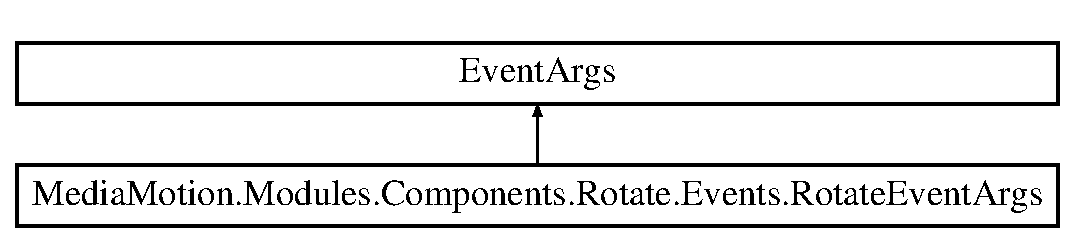
\includegraphics[height=2.000000cm]{class_media_motion_1_1_modules_1_1_components_1_1_rotate_1_1_events_1_1_rotate_event_args}
\end{center}
\end{figure}
\subsection*{Public Member Functions}
\begin{DoxyCompactItemize}
\item 
\hypertarget{class_media_motion_1_1_modules_1_1_components_1_1_rotate_1_1_events_1_1_rotate_event_args_af1273412151f15eda964d053552a0f41}{{\bfseries Rotate\+Event\+Args} (int Angle)}\label{class_media_motion_1_1_modules_1_1_components_1_1_rotate_1_1_events_1_1_rotate_event_args_af1273412151f15eda964d053552a0f41}

\end{DoxyCompactItemize}
\subsection*{Properties}
\begin{DoxyCompactItemize}
\item 
\hypertarget{class_media_motion_1_1_modules_1_1_components_1_1_rotate_1_1_events_1_1_rotate_event_args_a31665e411e7047ccc437601c3531f845}{int {\bfseries Angle}\hspace{0.3cm}{\ttfamily  \mbox{[}get\mbox{]}}}\label{class_media_motion_1_1_modules_1_1_components_1_1_rotate_1_1_events_1_1_rotate_event_args_a31665e411e7047ccc437601c3531f845}

\end{DoxyCompactItemize}


The documentation for this class was generated from the following file\+:\begin{DoxyCompactItemize}
\item 
O\+:/\+Projects/\+Media\+Motion/\+Media\+Motion/\+Assets/\+Scripts/\+Modules/\+Components/\+Rotate/\+Events/Rotate\+Event\+Args.\+cs\end{DoxyCompactItemize}

\hypertarget{class_media_motion_1_1_core_1_1_models_1_1_sound}{\section{Media\+Motion.\+Core.\+Models.\+Sound Class Reference}
\label{class_media_motion_1_1_core_1_1_models_1_1_sound}\index{Media\+Motion.\+Core.\+Models.\+Sound@{Media\+Motion.\+Core.\+Models.\+Sound}}
}
Inheritance diagram for Media\+Motion.\+Core.\+Models.\+Sound\+:\begin{figure}[H]
\begin{center}
\leavevmode
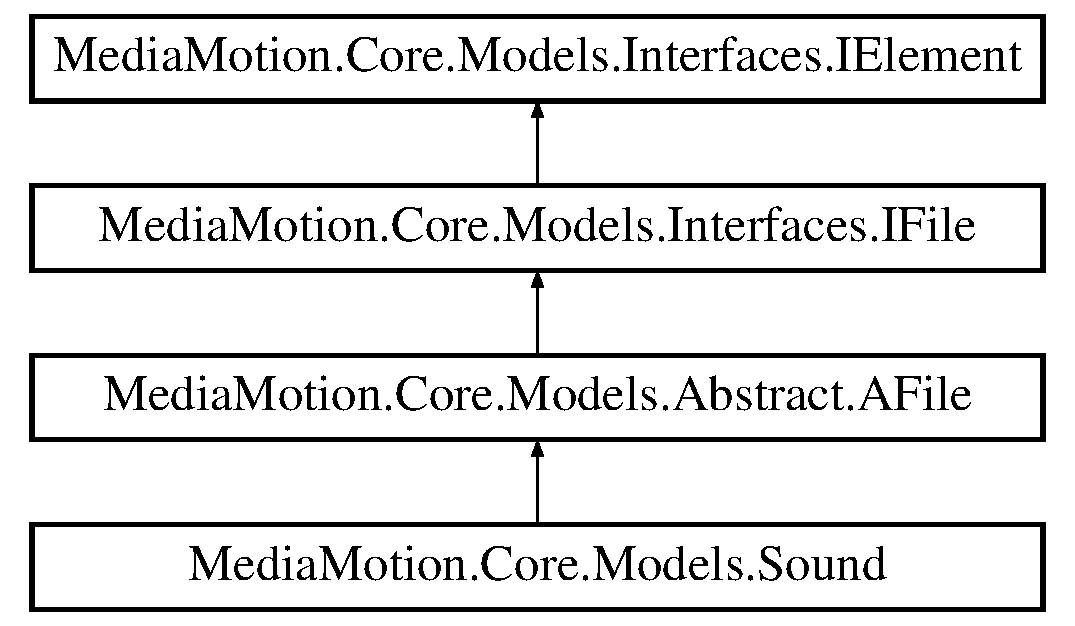
\includegraphics[height=4.000000cm]{class_media_motion_1_1_core_1_1_models_1_1_sound}
\end{center}
\end{figure}
\subsection*{Additional Inherited Members}


The documentation for this class was generated from the following file\+:\begin{DoxyCompactItemize}
\item 
O\+:/\+Projects/\+Media\+Motion/\+Media\+Motion/\+Assets/\+Scripts/\+Core/\+Models/\+File\+Manager/Sound.\+cs\end{DoxyCompactItemize}

\hypertarget{class_media_motion_1_1_core_1_1_models_1_1_text}{\section{Media\+Motion.\+Core.\+Models.\+Text Class Reference}
\label{class_media_motion_1_1_core_1_1_models_1_1_text}\index{Media\+Motion.\+Core.\+Models.\+Text@{Media\+Motion.\+Core.\+Models.\+Text}}
}
Inheritance diagram for Media\+Motion.\+Core.\+Models.\+Text\+:\begin{figure}[H]
\begin{center}
\leavevmode
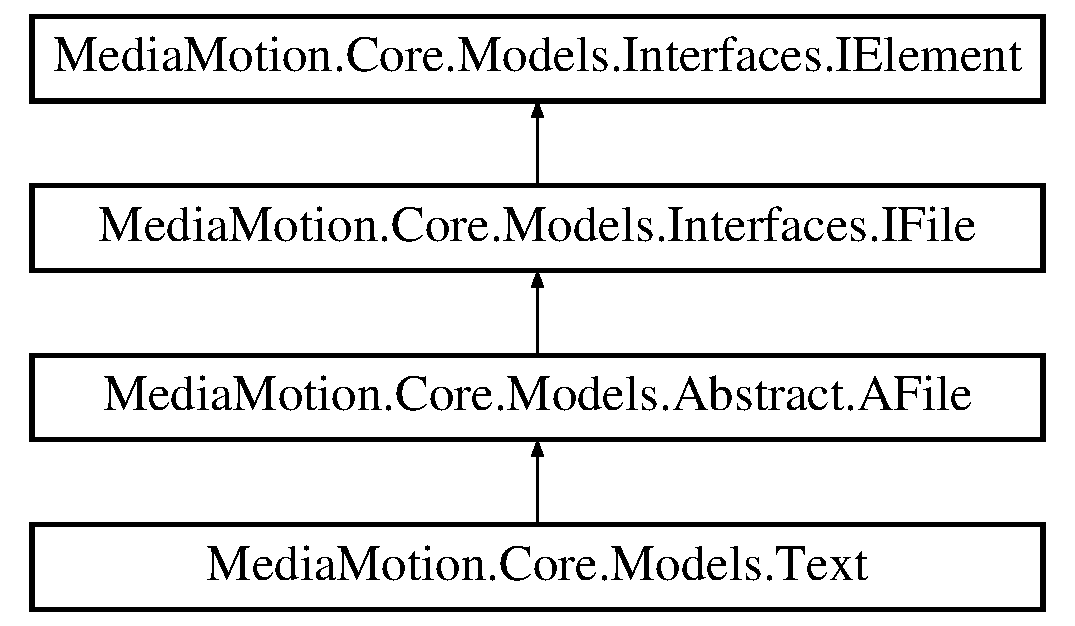
\includegraphics[height=4.000000cm]{class_media_motion_1_1_core_1_1_models_1_1_text}
\end{center}
\end{figure}
\subsection*{Additional Inherited Members}


The documentation for this class was generated from the following file\+:\begin{DoxyCompactItemize}
\item 
O\+:/\+Projects/\+Media\+Motion/\+Media\+Motion/\+Assets/\+Scripts/\+Core/\+Models/\+File\+Manager/Text.\+cs\end{DoxyCompactItemize}

\hypertarget{class_text_reader_u_i}{\section{Text\+Reader\+U\+I Class Reference}
\label{class_text_reader_u_i}\index{Text\+Reader\+U\+I@{Text\+Reader\+U\+I}}
}
Inheritance diagram for Text\+Reader\+U\+I\+:\begin{figure}[H]
\begin{center}
\leavevmode
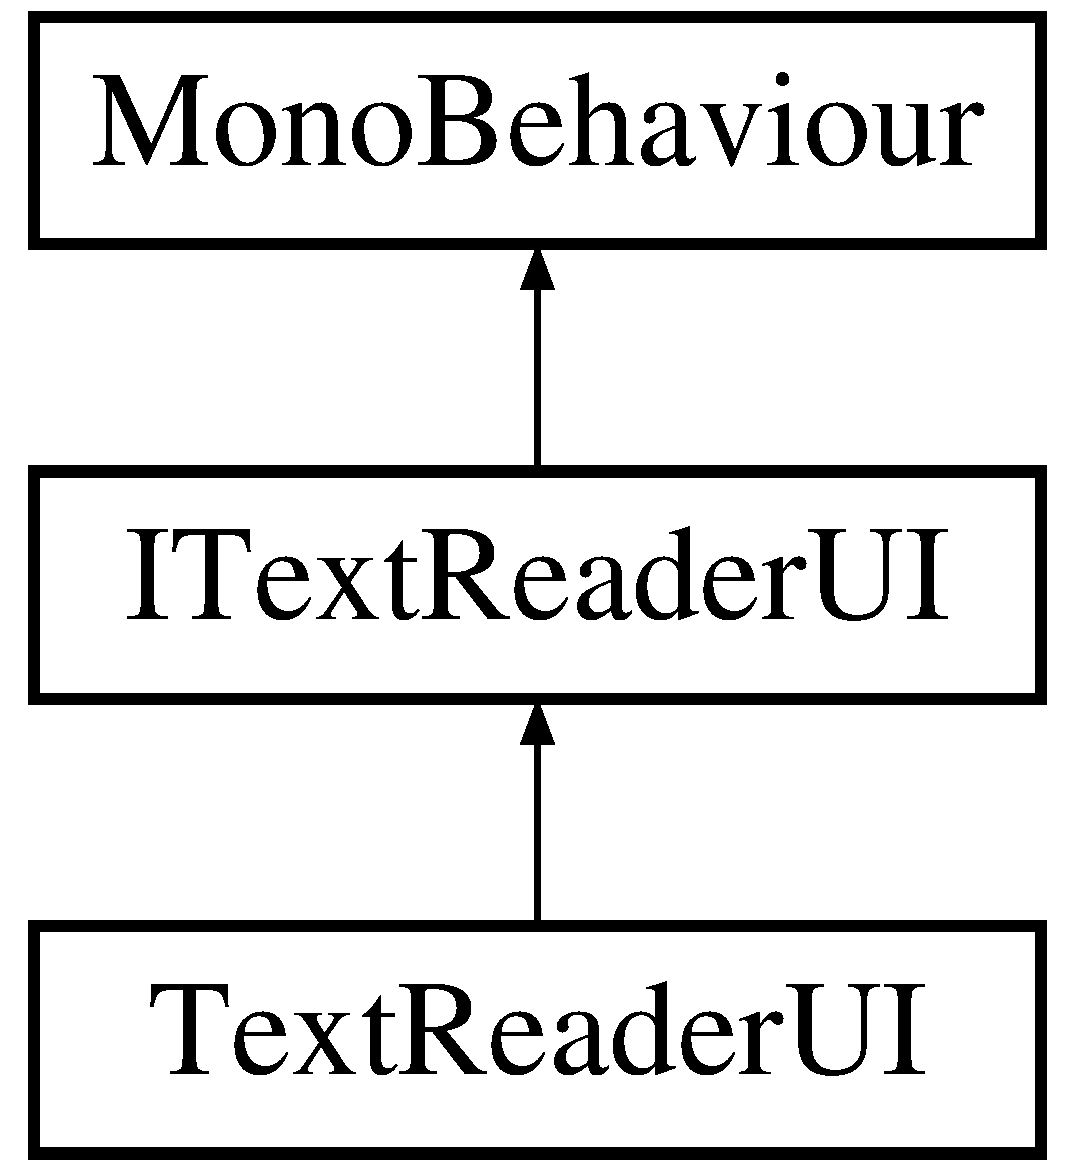
\includegraphics[height=3.000000cm]{class_text_reader_u_i}
\end{center}
\end{figure}
\subsection*{Additional Inherited Members}


The documentation for this class was generated from the following file\+:\begin{DoxyCompactItemize}
\item 
O\+:/\+Projects/\+Media\+Motion/\+Media\+Motion/\+Assets/\+Scripts/\+Core/\+View/Text\+Reader\+U\+I.\+cs\end{DoxyCompactItemize}

\hypertarget{class_media_motion_1_1_core_1_1_models_1_1_video}{\section{Media\+Motion.\+Core.\+Models.\+Video Class Reference}
\label{class_media_motion_1_1_core_1_1_models_1_1_video}\index{Media\+Motion.\+Core.\+Models.\+Video@{Media\+Motion.\+Core.\+Models.\+Video}}
}
Inheritance diagram for Media\+Motion.\+Core.\+Models.\+Video\+:\begin{figure}[H]
\begin{center}
\leavevmode
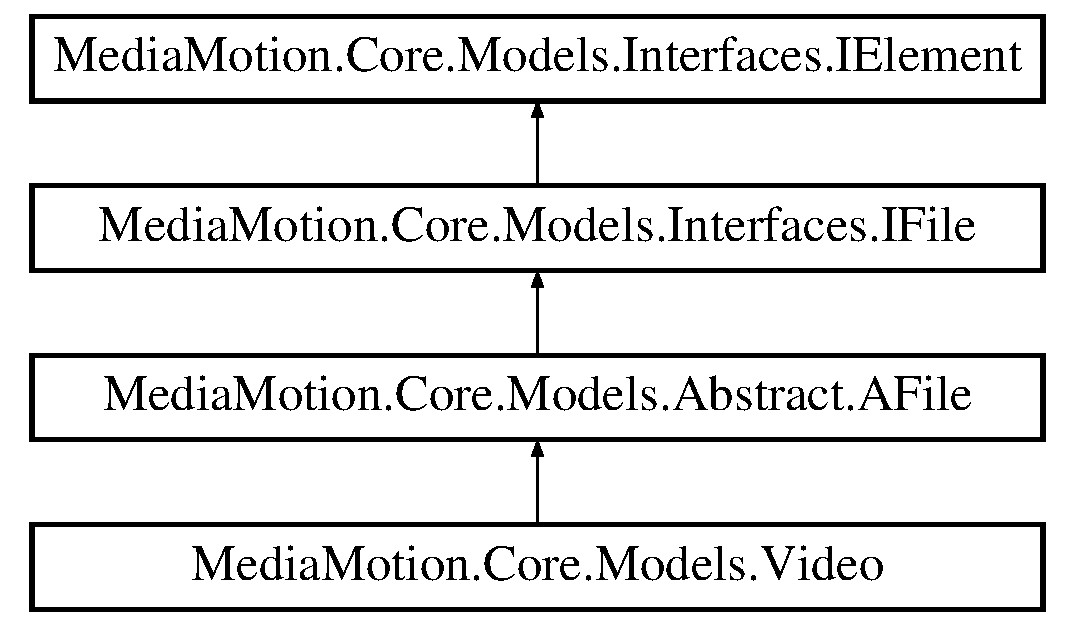
\includegraphics[height=4.000000cm]{class_media_motion_1_1_core_1_1_models_1_1_video}
\end{center}
\end{figure}
\subsection*{Additional Inherited Members}


The documentation for this class was generated from the following file\+:\begin{DoxyCompactItemize}
\item 
O\+:/\+Projects/\+Media\+Motion/\+Media\+Motion/\+Assets/\+Scripts/\+Core/\+Models/\+File\+Manager/Video.\+cs\end{DoxyCompactItemize}

\hypertarget{class_media_motion_1_1_modules_1_1_media_player_1_1_video_player_1_1_video_player}{\section{Media\+Motion.\+Modules.\+Media\+Player.\+Video\+Player.\+Video\+Player Class Reference}
\label{class_media_motion_1_1_modules_1_1_media_player_1_1_video_player_1_1_video_player}\index{Media\+Motion.\+Modules.\+Media\+Player.\+Video\+Player.\+Video\+Player@{Media\+Motion.\+Modules.\+Media\+Player.\+Video\+Player.\+Video\+Player}}
}
Inheritance diagram for Media\+Motion.\+Modules.\+Media\+Player.\+Video\+Player.\+Video\+Player\+:\begin{figure}[H]
\begin{center}
\leavevmode
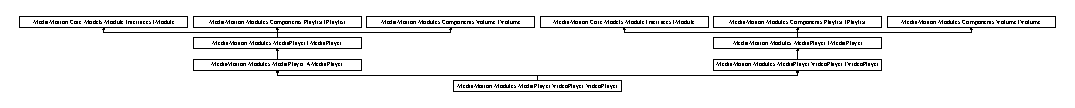
\includegraphics[height=1.003584cm]{class_media_motion_1_1_modules_1_1_media_player_1_1_video_player_1_1_video_player}
\end{center}
\end{figure}
\subsection*{Public Member Functions}
\begin{DoxyCompactItemize}
\item 
\hypertarget{class_media_motion_1_1_modules_1_1_media_player_1_1_video_player_1_1_video_player_af73fa88a47e81aad8f22de016af2d2cc}{override void {\bfseries Play} ()}\label{class_media_motion_1_1_modules_1_1_media_player_1_1_video_player_1_1_video_player_af73fa88a47e81aad8f22de016af2d2cc}

\item 
\hypertarget{class_media_motion_1_1_modules_1_1_media_player_1_1_video_player_1_1_video_player_ac39e814e464f19810c70311b90142ba0}{override void {\bfseries Pause} ()}\label{class_media_motion_1_1_modules_1_1_media_player_1_1_video_player_1_1_video_player_ac39e814e464f19810c70311b90142ba0}

\item 
\hypertarget{class_media_motion_1_1_modules_1_1_media_player_1_1_video_player_1_1_video_player_ae10124ec1557936c846c565ca39da1c0}{override void {\bfseries Stop} ()}\label{class_media_motion_1_1_modules_1_1_media_player_1_1_video_player_1_1_video_player_ae10124ec1557936c846c565ca39da1c0}

\end{DoxyCompactItemize}
\subsection*{Additional Inherited Members}


The documentation for this class was generated from the following file\+:\begin{DoxyCompactItemize}
\item 
O\+:/\+Projects/\+Media\+Motion/\+Media\+Motion/\+Assets/\+Scripts/\+Modules/\+Media\+Player/\+Video\+Player/Video\+Player.\+cs\end{DoxyCompactItemize}

\hypertarget{class_media_motion_1_1_modules_1_1_components_1_1_volume_1_1_volume}{\section{Media\+Motion.\+Modules.\+Components.\+Volume.\+Volume Class Reference}
\label{class_media_motion_1_1_modules_1_1_components_1_1_volume_1_1_volume}\index{Media\+Motion.\+Modules.\+Components.\+Volume.\+Volume@{Media\+Motion.\+Modules.\+Components.\+Volume.\+Volume}}
}
Inheritance diagram for Media\+Motion.\+Modules.\+Components.\+Volume.\+Volume\+:\begin{figure}[H]
\begin{center}
\leavevmode
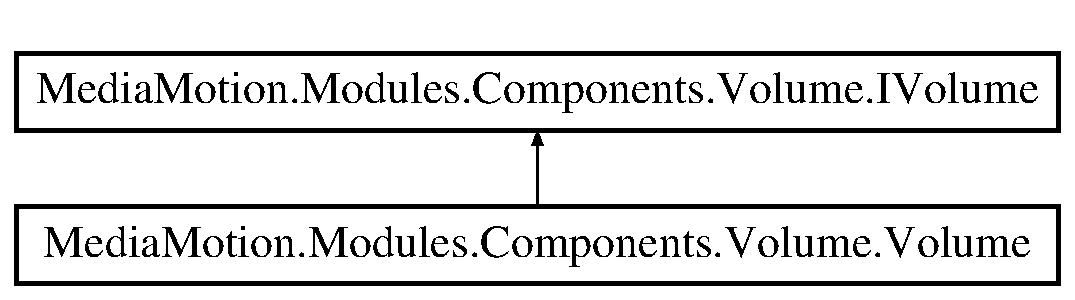
\includegraphics[height=2.000000cm]{class_media_motion_1_1_modules_1_1_components_1_1_volume_1_1_volume}
\end{center}
\end{figure}
\subsection*{Public Member Functions}
\begin{DoxyCompactItemize}
\item 
\hypertarget{class_media_motion_1_1_modules_1_1_components_1_1_volume_1_1_volume_aa139af6299f07c6cd565463ddd656aef}{delegate void {\bfseries Volume\+Change\+Handler} (object sender, \hyperlink{class_media_motion_1_1_modules_1_1_components_1_1_volume_1_1_events_1_1_volume_change_event_args}{Volume\+Change\+Event\+Args} e)}\label{class_media_motion_1_1_modules_1_1_components_1_1_volume_1_1_volume_aa139af6299f07c6cd565463ddd656aef}

\item 
\hypertarget{class_media_motion_1_1_modules_1_1_components_1_1_volume_1_1_volume_a78ee24429301cb6f0dbed70e61401951}{void {\bfseries Volume\+Up} ()}\label{class_media_motion_1_1_modules_1_1_components_1_1_volume_1_1_volume_a78ee24429301cb6f0dbed70e61401951}

\item 
\hypertarget{class_media_motion_1_1_modules_1_1_components_1_1_volume_1_1_volume_af1d1a2f2cec6adda05edbb5411a96628}{void {\bfseries Volume\+Down} ()}\label{class_media_motion_1_1_modules_1_1_components_1_1_volume_1_1_volume_af1d1a2f2cec6adda05edbb5411a96628}

\end{DoxyCompactItemize}
\subsection*{Properties}
\begin{DoxyCompactItemize}
\item 
\hypertarget{class_media_motion_1_1_modules_1_1_components_1_1_volume_1_1_volume_aa2b04930f2feeda79d381e662389e9e6}{int {\bfseries Sound}\hspace{0.3cm}{\ttfamily  \mbox{[}get\mbox{]}}}\label{class_media_motion_1_1_modules_1_1_components_1_1_volume_1_1_volume_aa2b04930f2feeda79d381e662389e9e6}

\item 
\hypertarget{class_media_motion_1_1_modules_1_1_components_1_1_volume_1_1_volume_a6553c285b133d2db698b953ad0da978e}{int {\bfseries Step}\hspace{0.3cm}{\ttfamily  \mbox{[}get\mbox{]}}}\label{class_media_motion_1_1_modules_1_1_components_1_1_volume_1_1_volume_a6553c285b133d2db698b953ad0da978e}

\end{DoxyCompactItemize}
\subsection*{Events}
\begin{DoxyCompactItemize}
\item 
\hypertarget{class_media_motion_1_1_modules_1_1_components_1_1_volume_1_1_volume_a3e93fb0d13bc06da2515736071f458c8}{Volume\+Change\+Handler {\bfseries On\+Volume\+Change}}\label{class_media_motion_1_1_modules_1_1_components_1_1_volume_1_1_volume_a3e93fb0d13bc06da2515736071f458c8}

\end{DoxyCompactItemize}


The documentation for this class was generated from the following file\+:\begin{DoxyCompactItemize}
\item 
O\+:/\+Projects/\+Media\+Motion/\+Media\+Motion/\+Assets/\+Scripts/\+Modules/\+Components/\+Volume/Volume.\+cs\end{DoxyCompactItemize}

\hypertarget{class_media_motion_1_1_modules_1_1_components_1_1_volume_1_1_events_1_1_volume_change_event_args}{\section{Media\+Motion.\+Modules.\+Components.\+Volume.\+Events.\+Volume\+Change\+Event\+Args Class Reference}
\label{class_media_motion_1_1_modules_1_1_components_1_1_volume_1_1_events_1_1_volume_change_event_args}\index{Media\+Motion.\+Modules.\+Components.\+Volume.\+Events.\+Volume\+Change\+Event\+Args@{Media\+Motion.\+Modules.\+Components.\+Volume.\+Events.\+Volume\+Change\+Event\+Args}}
}
Inheritance diagram for Media\+Motion.\+Modules.\+Components.\+Volume.\+Events.\+Volume\+Change\+Event\+Args\+:\begin{figure}[H]
\begin{center}
\leavevmode
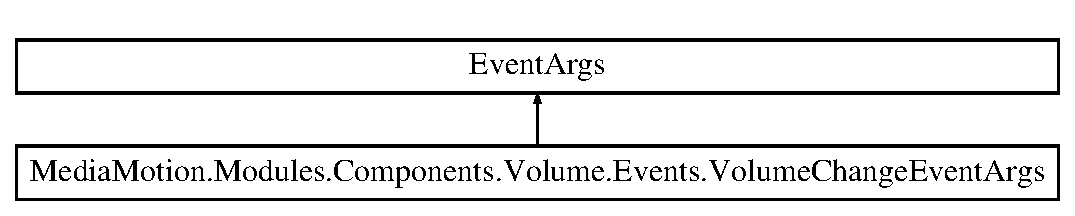
\includegraphics[height=2.000000cm]{class_media_motion_1_1_modules_1_1_components_1_1_volume_1_1_events_1_1_volume_change_event_args}
\end{center}
\end{figure}
\subsection*{Public Member Functions}
\begin{DoxyCompactItemize}
\item 
\hypertarget{class_media_motion_1_1_modules_1_1_components_1_1_volume_1_1_events_1_1_volume_change_event_args_a4a9db792753615ff8082da56203cdaf4}{{\bfseries Volume\+Change\+Event\+Args} (int New\+Volume)}\label{class_media_motion_1_1_modules_1_1_components_1_1_volume_1_1_events_1_1_volume_change_event_args_a4a9db792753615ff8082da56203cdaf4}

\end{DoxyCompactItemize}
\subsection*{Properties}
\begin{DoxyCompactItemize}
\item 
\hypertarget{class_media_motion_1_1_modules_1_1_components_1_1_volume_1_1_events_1_1_volume_change_event_args_abaa32dffd46ba9d89087da5bb65d3adc}{int {\bfseries Volume}\hspace{0.3cm}{\ttfamily  \mbox{[}get\mbox{]}}}\label{class_media_motion_1_1_modules_1_1_components_1_1_volume_1_1_events_1_1_volume_change_event_args_abaa32dffd46ba9d89087da5bb65d3adc}

\end{DoxyCompactItemize}


The documentation for this class was generated from the following file\+:\begin{DoxyCompactItemize}
\item 
O\+:/\+Projects/\+Media\+Motion/\+Media\+Motion/\+Assets/\+Scripts/\+Modules/\+Components/\+Volume/\+Events/Volume\+Change\+Event\+Args.\+cs\end{DoxyCompactItemize}

\hypertarget{class_media_motion_1_1_core_1_1_controllers_1_1_wheel_tool_controller}{\section{Media\+Motion.\+Core.\+Controllers.\+Wheel\+Tool\+Controller Class Reference}
\label{class_media_motion_1_1_core_1_1_controllers_1_1_wheel_tool_controller}\index{Media\+Motion.\+Core.\+Controllers.\+Wheel\+Tool\+Controller@{Media\+Motion.\+Core.\+Controllers.\+Wheel\+Tool\+Controller}}
}
Inheritance diagram for Media\+Motion.\+Core.\+Controllers.\+Wheel\+Tool\+Controller\+:\begin{figure}[H]
\begin{center}
\leavevmode
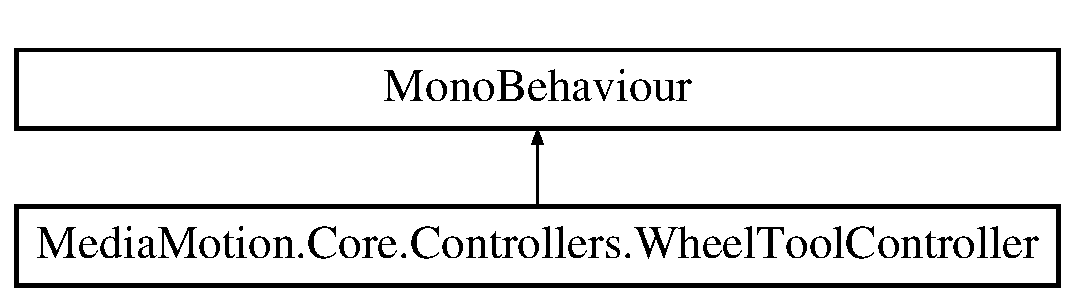
\includegraphics[height=2.000000cm]{class_media_motion_1_1_core_1_1_controllers_1_1_wheel_tool_controller}
\end{center}
\end{figure}


The documentation for this class was generated from the following file\+:\begin{DoxyCompactItemize}
\item 
O\+:/\+Projects/\+Media\+Motion/\+Media\+Motion/\+Assets/\+Scripts/\+Core/\+Controllers/Wheel\+Tool\+Controller.\+cs\end{DoxyCompactItemize}

\hypertarget{class_wheel_tool_u_i}{\section{Wheel\+Tool\+U\+I Class Reference}
\label{class_wheel_tool_u_i}\index{Wheel\+Tool\+U\+I@{Wheel\+Tool\+U\+I}}
}
Inheritance diagram for Wheel\+Tool\+U\+I\+:\begin{figure}[H]
\begin{center}
\leavevmode
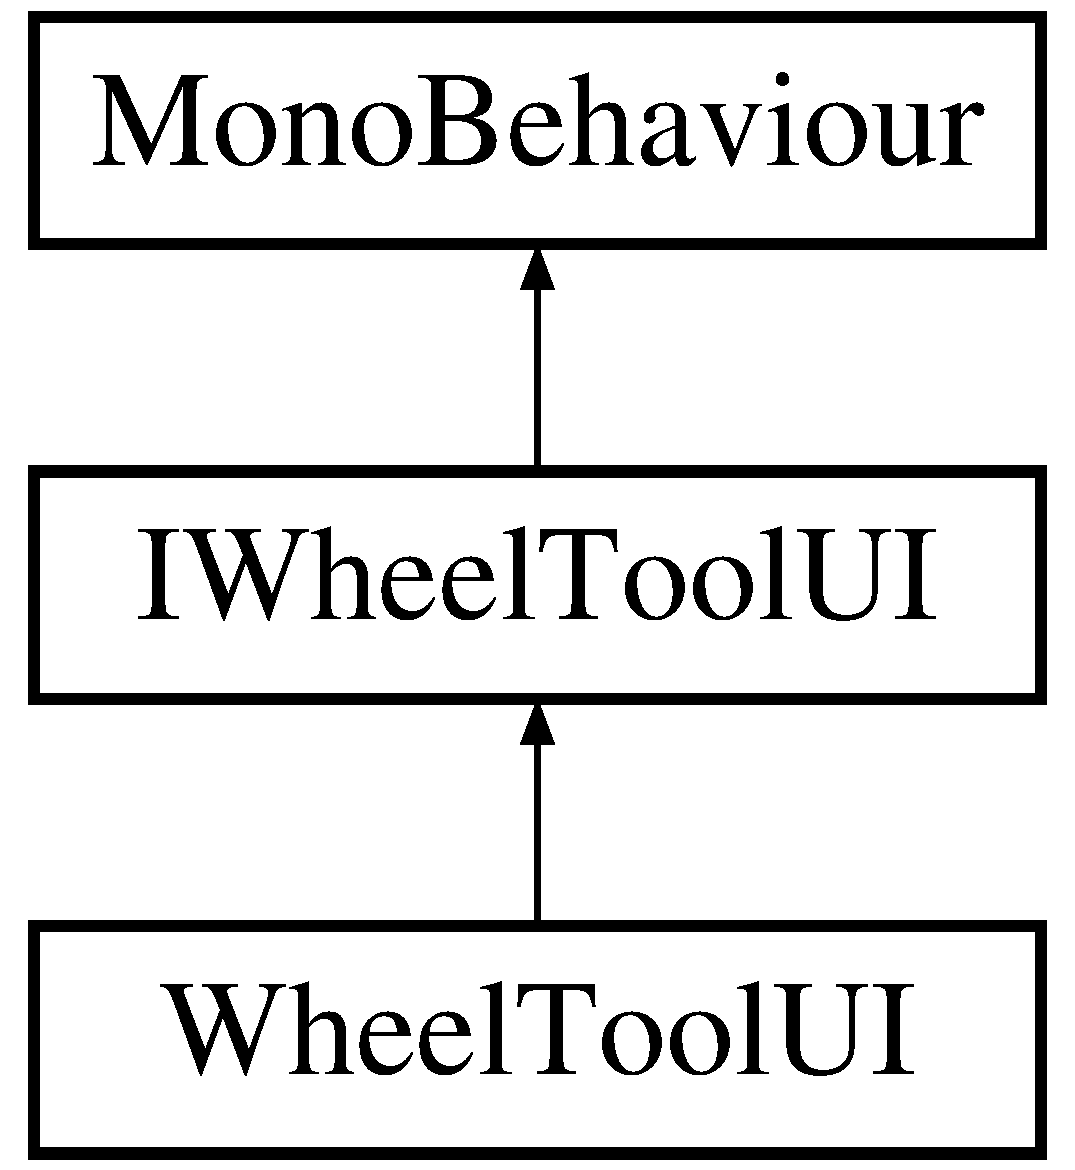
\includegraphics[height=3.000000cm]{class_wheel_tool_u_i}
\end{center}
\end{figure}
\subsection*{Additional Inherited Members}


The documentation for this class was generated from the following file\+:\begin{DoxyCompactItemize}
\item 
O\+:/\+Projects/\+Media\+Motion/\+Media\+Motion/\+Assets/\+Scripts/\+Core/\+View/Wheel\+Tool\+U\+I.\+cs\end{DoxyCompactItemize}

\hypertarget{class_media_motion_1_1_modules_1_1_components_1_1_zoom_1_1_zoom}{\section{Media\+Motion.\+Modules.\+Components.\+Zoom.\+Zoom Class Reference}
\label{class_media_motion_1_1_modules_1_1_components_1_1_zoom_1_1_zoom}\index{Media\+Motion.\+Modules.\+Components.\+Zoom.\+Zoom@{Media\+Motion.\+Modules.\+Components.\+Zoom.\+Zoom}}
}
\subsection*{Public Member Functions}
\begin{DoxyCompactItemize}
\item 
\hypertarget{class_media_motion_1_1_modules_1_1_components_1_1_zoom_1_1_zoom_a8852d656a38cf63f2a925081331d776a}{delegate void {\bfseries Zoom\+Handler} (object sender, \hyperlink{class_media_motion_1_1_modules_1_1_components_1_1_zoom_1_1_events_1_1_zoom_event_args}{Zoom\+Event\+Args} e)}\label{class_media_motion_1_1_modules_1_1_components_1_1_zoom_1_1_zoom_a8852d656a38cf63f2a925081331d776a}

\item 
\hypertarget{class_media_motion_1_1_modules_1_1_components_1_1_zoom_1_1_zoom_a18f758cb3e09c6d7b5e185e5ae3567f6}{void {\bfseries Zoom\+In} ()}\label{class_media_motion_1_1_modules_1_1_components_1_1_zoom_1_1_zoom_a18f758cb3e09c6d7b5e185e5ae3567f6}

\item 
\hypertarget{class_media_motion_1_1_modules_1_1_components_1_1_zoom_1_1_zoom_ad1ef765101ff933dedcfb27a37fc2b3e}{void {\bfseries Zoom\+Out} ()}\label{class_media_motion_1_1_modules_1_1_components_1_1_zoom_1_1_zoom_ad1ef765101ff933dedcfb27a37fc2b3e}

\end{DoxyCompactItemize}
\subsection*{Properties}
\begin{DoxyCompactItemize}
\item 
\hypertarget{class_media_motion_1_1_modules_1_1_components_1_1_zoom_1_1_zoom_a0367d9e6cfc175cf7da89eac7e9bafb0}{float {\bfseries Coeff}\hspace{0.3cm}{\ttfamily  \mbox{[}get\mbox{]}}}\label{class_media_motion_1_1_modules_1_1_components_1_1_zoom_1_1_zoom_a0367d9e6cfc175cf7da89eac7e9bafb0}

\end{DoxyCompactItemize}
\subsection*{Events}
\begin{DoxyCompactItemize}
\item 
\hypertarget{class_media_motion_1_1_modules_1_1_components_1_1_zoom_1_1_zoom_a708fe5bd74db3942d16ede7ac4da75e3}{Zoom\+Handler {\bfseries On\+Zoom}}\label{class_media_motion_1_1_modules_1_1_components_1_1_zoom_1_1_zoom_a708fe5bd74db3942d16ede7ac4da75e3}

\end{DoxyCompactItemize}


The documentation for this class was generated from the following file\+:\begin{DoxyCompactItemize}
\item 
O\+:/\+Projects/\+Media\+Motion/\+Media\+Motion/\+Assets/\+Scripts/\+Modules/\+Components/\+Zoom/Zoom.\+cs\end{DoxyCompactItemize}

\hypertarget{class_media_motion_1_1_modules_1_1_components_1_1_zoom_1_1_events_1_1_zoom_event_args}{\section{Media\+Motion.\+Modules.\+Components.\+Zoom.\+Events.\+Zoom\+Event\+Args Class Reference}
\label{class_media_motion_1_1_modules_1_1_components_1_1_zoom_1_1_events_1_1_zoom_event_args}\index{Media\+Motion.\+Modules.\+Components.\+Zoom.\+Events.\+Zoom\+Event\+Args@{Media\+Motion.\+Modules.\+Components.\+Zoom.\+Events.\+Zoom\+Event\+Args}}
}
Inheritance diagram for Media\+Motion.\+Modules.\+Components.\+Zoom.\+Events.\+Zoom\+Event\+Args\+:\begin{figure}[H]
\begin{center}
\leavevmode
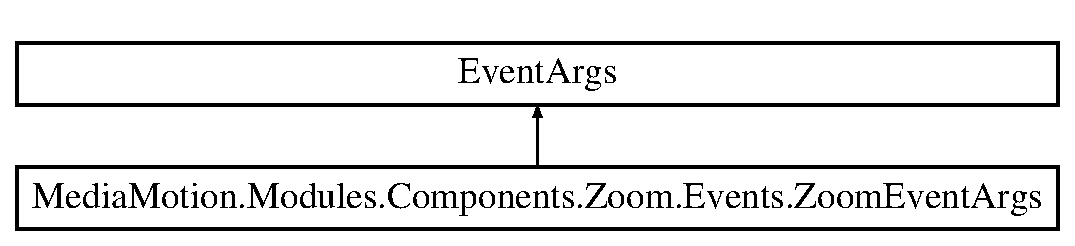
\includegraphics[height=2.000000cm]{class_media_motion_1_1_modules_1_1_components_1_1_zoom_1_1_events_1_1_zoom_event_args}
\end{center}
\end{figure}
\subsection*{Public Member Functions}
\begin{DoxyCompactItemize}
\item 
\hypertarget{class_media_motion_1_1_modules_1_1_components_1_1_zoom_1_1_events_1_1_zoom_event_args_ac361061684d193b18543ef0ed0f66384}{{\bfseries Zoom\+Event\+Args} (float \hyperlink{class_media_motion_1_1_modules_1_1_components_1_1_zoom_1_1_zoom}{Zoom})}\label{class_media_motion_1_1_modules_1_1_components_1_1_zoom_1_1_events_1_1_zoom_event_args_ac361061684d193b18543ef0ed0f66384}

\end{DoxyCompactItemize}
\subsection*{Properties}
\begin{DoxyCompactItemize}
\item 
\hypertarget{class_media_motion_1_1_modules_1_1_components_1_1_zoom_1_1_events_1_1_zoom_event_args_a40d897e8f6ef604215b4db2ca0066258}{float {\bfseries Zoom}\hspace{0.3cm}{\ttfamily  \mbox{[}get\mbox{]}}}\label{class_media_motion_1_1_modules_1_1_components_1_1_zoom_1_1_events_1_1_zoom_event_args_a40d897e8f6ef604215b4db2ca0066258}

\end{DoxyCompactItemize}


The documentation for this class was generated from the following file\+:\begin{DoxyCompactItemize}
\item 
O\+:/\+Projects/\+Media\+Motion/\+Media\+Motion/\+Assets/\+Scripts/\+Modules/\+Components/\+Zoom/\+Events/Zoom\+Event\+Args.\+cs\end{DoxyCompactItemize}

%--- End generated contents ---

% Index
\newpage
\phantomsection
\addcontentsline{toc}{chapter}{Index}
\printindex

\end{document}
